\documentclass[a4paper,14pt]{extreport}
\usepackage[utf8]{inputenc}


%Language&Font
%Geometry
\setcounter{secnumdepth}{4}
\setcounter{tocdepth}{3}
\usepackage[left=2cm,right=2cm,
    top=2cm,bottom=2cm,bindingoffset=0cm]{geometry}
\usepackage{breqn}
\linespread{1.3}
\usepackage[ukrainian]{babel}
%\setmainfont{Times New Roman}
%\usepackage{lmodern} 
\usepackage[T1]{fontenc}
\usepackage{layouts}
\usepackage{lipsum}


%========================================
%Table
\usepackage{booktabs, multirow} % for borders and merged ranges
\usepackage{soul}% for underlines
\usepackage[table]{xcolor} % for cell colors
\usepackage{changepage,threeparttable} % for wide tables

%========================================
%Math
\usepackage{mathtools}
\usepackage{float}
\usepackage{amsmath}
\newcommand{\angstrom}{\text{\normalfont\AA}}
%========================================
%Pictures
\usepackage{svg}
\usepackage{pgfplots}
\usepackage{graphicx}
\graphicspath{{img/}}
\DeclareGraphicsExtensions{.pdf,.png,.jpg,.eps, .svg, pgf}
\usepackage{caption}
\usepackage{subcaption}
\usepackage{hyperref}
\DeclareCaptionType{constrains}[Список][Список]

%========================================
%Титулка
%\title{Дипломна робота}
%\author{Носенко Артем Олексійович}
%\date{December 2021}


%========================================
%Table contents
\bibliographystyle{ieeetr}
\usepackage{hyperref}
\hypersetup{
    colorlinks,
    citecolor=black,
    filecolor=black,
    linkcolor=black,
    urlcolor=black
}

%========================================
%Body
\begin{document}
%\begin{titlepage}
%  \renewcommand\baselinestretch{0.75}\normalsize
%  \renewcommand\baselinestretch{1.25}\normalsize
 \begin{center}
Національна академія наук України \\
Міністерство освіти і науки України
  \vspace{0.25cm}
  
  \textbf{Державна наукова установа \\ 
  «Київський академічний університет»}
  \vspace{0.5cm}
  
  Кафедра прикладної фізики та наноматеріалів
  \\ Спеціальність 105 Прикладна фізика та наноматеріали
  
  \vspace{1cm}
  
  \large\textbf{МАГІСТЕРСЬКА  ДИПЛОМНА  РОБОТА} \\
  студента  \textbf{Носенка Артема Олексійовича}
 \end{center}
\begin{center}
 {На тему \large\textbf{«Моделювання електронної структури Ван-дер-Ваальсових матеріалів в межах ТФГ»}\par}
\end{center}
\vspace{0.5cm}

\hfill\parbox{12cm}{
\begin{flushleft}
 \hfill Науковий керівник: доктор фіз.-мат. наук, професор \\
 \hfill \underline{\hspace{4cm}} \hspace{1cm} Карбівський В. Л. \\
 \hfill Рецензент: доктор фіз.-мат. наук, професор \\
 \hfill \underline{\hspace{4cm}} \hspace{2cm} Хижун О. Ю. \\
\end{flushleft}}

\hfill\parbox{10cm}{
\begin{flushleft}
 \begin{center}
 \small
     \textbf{Робота допущена до захисту в ЕК} \\
     Завідувач кафедри \\
     доктор фіз.-мат. наук, професор \\
     \hfill \underline{\hspace{4cm}} \hspace{1cm} Лень Є. Г.  
 \end{center}
\end{flushleft}}

\hfill\parbox{10cm}{
\begin{flushleft}
 \begin{center}
 \small
     Засвідчую, що у цій магістерській роботі немає 
     запозичень з праць інших авторів без відповідних посилань \\
     Студент \underline{\hspace{4cm}} Носенко А. О.
 \end{center}
\end{flushleft}}

\vfill

\begin{center}
 Київ -- 2022
\end{center}
\end{titlepage}
\tableofcontents
\begin{center}
{\large \textbf{АНОТАЦІЯ}}
\end{center}

\textbf{Носенко А. О.} Моделювання електронної структури Ван-дер-Ваальсових матеріалів в межах DFT. \\
Кваліфікаційна робота магістра за спеціальністю 105 Прикдна фізика і наноматеріали, освітня програма Пркикладна фізика і наноматеріали. 
"--- Державна наукова установа «Київський академічний університет», кафедра прикладної фізики та наноматеріалів. "--- Київ "--- 2022.

\textbf{Науковий керівник}: д.ф.-м.н. Карбівський В. Л.

\textbf{Ключові слова}: діхалькогеніди перехідних металів, зонні розрахунки, теорія функціонала густини

\textbf{Елементи оформлення}: 13 рисунків, 4 таблиць, 1 список.

Використовуючи в рамках теорії функціонала густини підходи GGA в PBE параметризації та meta-GGA в SCAN параметризації, було визначено оптимальні параметри розрахунків електронних властивостей, зокрема визначили оптимальний параметр Хаббардовської взаємодії U, дихалькогенідів перехідних металів 1T-TiX$_2$ (X = S, Se, Te). Встановили електронну природу 1T-TiS$_2$, 1T-TiSe$_2$, 1T-TiTe$_2$ та розрахувати ширину забороненої зони для 1T-TiS$_2$. 



\bigskip

\clearpage

\thispagestyle{empty}
\begin{center}
{\large \textbf{SUMMARY}}
\end{center}

\textbf{Nosenko A. O.} Modeling of the electronic structure of van der Waals materials by means DFT. \\
Masters qualification work in specialty 105 Applied physics and nanomaterials, educational program Applied physics and nanomaterials "--- State Research Institution «Kyiv Academic University», Department of Applied physics and nanomaterials. "--- Kyiv "--- 2022.

\textbf{Research supervisor}: Doctor of Physical and Mathematical Sciences, \\ Karbivsky V. L.

\textbf{Key words}: transition metal dichalcogenides, band calculations, density functional theory

\textbf{Design elements}: 13 Figures, 4 Tables, 1 list.

Using the GGA approaches in PBE parameterization and meta-GGA in SCAN parameterization within the framework of density functional theory, optimal parameters for calculating electronic properties were determined, in particular, the optimal parameter of the Hubbard interaction U for transition metal dichalcogenides 1T-TiX$_2$. (X = s, Se, Te) was determined. We have established the electronic nature of 1T-TiS$_2$, 1T-TiSe$_2$, 1T-TiTe$_2$ and calculated the width of the gap for 1T-TiS$_2$.
\chapter{Вступ}
Після відкриття А. Геймом та К. Новосьоловим графену у 2004 році \cite{Graphene}, знову зріс інтерес до двохвимірних матеріалів, зокрема до дихалькогенідів перехідних металів (Transition metal dichalcogenides) та їх інтеркаляційних сполук, які дуже сильно досліджувались у 80-х роках. Ці сполуки мають формулу MX$_{2}$ (X = S, Se, Te; M = Ti, Zr, Hf, V, Nb, Ta, Mo, W). TMDs складаються з складених тришарових X-M-X і мають гексагональну або тригональну симетрію. Ці тришарові шари утримуються разом слабкими силами ван-дер-Ваальса, що дозволяє відшаровувати окремі тришарові шари і осаджувати ці шари на різні підкладки. Цей простий метод отримання наноструктур у поєднанні з багатими фізичними властивостями TMD роблять їх перспективними матеріалами для спінтроніки, наноелектроніки, виробництва відновлюваної енергії, біохімічних застосувань, а також для valleytronics – абсолютно нового підходу до квантових обчислень.

Ключовою особливістю, загальною для багатьох матеріалів TMD, є впорядкування хвилі щільності заряду (CDW), яке часто виникає поблизу надпровідності. Типовим прикладом є 1T-TiSe$_2$, в якому перехід у стан CDW відбувається при CDW ~ 200K. Нижче TCDW TiSe$_2$ кристалізується в форму надрешітки 2x2x2 CDW з симетрією P-3c1 (165 просторова симетрія), в той час, як неспотворений кристал при T > T$_{CDW}$ має симетрію P-3m1 (164 просторова симетрія). Нижче переходу питомий опір сильно зростає.

Споріднені сполуки 1T-TiS$_2$ і 1T-TiTe$_2$ отримують з TiSe$_2$ шляхом ізовалентної заміни Te і S На Se відповідно. Сполуки мають ту ж кристалічну структуру, що і 1T-TiSe$_2$ в умовах навколишнього середовища. Однак, на відміну від TiSe$_2$, 1T-TiTe$_2$ не проявляє ніякого CDW в об'ємі при низьких температурах. Нещодавно було показано, що (2x2) CDW може з'являтися тільки в моношарах TiTe2 (P. Chen та ін.). Експериментальна ситуація з TiS$_2$ більш суперечлива. Досі обговорюється, чи має він напівпровідникову або напівметалічну природу. Частина фазової діаграми TiSe$_2$--$_x$S$_x$ до X < 0,34 була нещодавно вивчена за допомогою ARPES і STM. Автори бачили, що CDW поступово пригнічується. Екстраполюючи свої результати, автори дійшли висновку, що CDW звертається в нуль при легуванні, близькому до x = 1.

Оскільки модуляція щільності заряду та спотворення структури в стані CDW відбуваються одночасно, рушійна сила переходу CDW все ще обговорюється. Було запропоновано кілька механізмів, включаючи фононну конденсацію, екситонний механізм, зонну нестійкість Яна-Теллера, орбітальне впорядкування, взаємодія нестійкостей Купера і частинок-дірок.

Метою даної роботи є вивчення зонної структури основного стану сполук TiS$_2$ TiSe$_2$ TiTe$_2$ за допомогою meta-GGA функціоналів з включенням Хаббардовської взаємодії. 

\section{Літературній огляд досліджуваних систем}
\subsection{TiS2}
Дослідження електронної будови TiS$_{2}$ дали суперечливі висновки. З одного боку деякі розрахунки зонної структури приводять до непрямого перекриття p/d смуг між точками $\Gamma$ та $L$ в діапазоні від 0.2 до 1,5 еВ. Інші стверджують, що TiS$_{2}$ є вузько-щілинним напівпровідником. Експериментальні данні отримані за допомогою фотоемісії вказують на те, що поведінка даної сполуки схожа на напівпровідникову \cite{semiconducter} або ж напівметалічну \cite{semimetal}. Як відомо, TiS$_{2}$ має високу електронну провідність без зовнішнього легування, однак походження цієї високої провідності, будь то напівметал або сильно легований напівпровідник, обговорюється протягом декількох десятиліть, але деякі недавні GW, DFT розрахунки в поєднані з сканувальною зондовою мікроскопією, все ж таки, стверджують, що висока провідність обумовлена сильним самолегуванням \cite{semimetal_or_semiconducter}. 

Щодо прикладного застосування, то даний матеріал успішно використовується у літій-іонних акумуляторах у якості катода. Коефіцієнт дифузії літію у TiS$_2$ порядку $10^{-8}-10^{-7}$ см$^2$/с, на один --- два порядки вище, ніж у широко використовуваних оксидних катодів. Недавні досліди показують, що комірки TiS$_2$ могуть зберігати більш ніж 50 \% початкової ємності після 35 років зберігання. Однією з важливих причин, чому TiS$_2$ був обраний як катодний матеріал для літій-іонних батарей, є те, що він має високу внутрішню електропровідність без зовнішнього легування. Це відрізняється від деяких інших популярних катодів таких, як LiFePO$_4$, для яких низька провідність була головною проблемою.

У 2003 році метод низькотемпературного газофазного синтезу(TiCl$_4$ + 2H$_2$S $\rightarrow$ TiS$_2$ + 4HCl), був успішно використаний для отримання нанотрубок на основі TiS$_2$ \cite{nanotube}. Аналіз їх морфології і структури показав, що трубки складаються з співвісних шарів сульфіду титану (відстань між шарами становить 0,57 нм) з атомним співвідношенням Ti:S =1:2, мають відкриті кінці, середні значення зовнішнього і внутрішнього діаметрів трубок складають  20 - 30 і  10 нм відповідно. У роботах \cite{nanotube2,nanotube3} були вивчені процеси інтеркалювання нанотрубок TiS$_2$ літієм і воднем і обговорені можливості їх використання в якості матеріалів для водневих акумуляторів. Матеріалознавчі перспективи різних класів наноструктур багато в чому визначаються їх електронними властивостями, які можуть істотно відрізнятися від відповідних кристалічних (3D) фаз. Зазначені властивості в свою чергу залежать від атомної будови і геометрії наноструктур. Так, нанотрубки дисульфідів Mo, W є напівпровідниками, причому в залежності від діаметра і атомної конфігурації стінок (так званої хіральності) величина забороненої щілини різко змінюється. Навпаки, всі NbS$_2$-нанотрубки за своїми провідними властивостями є металами \cite{nanotube4,nanotube5,nanotube6}.
\subsection{TiSe2}
Діхалькогеніди перехідних металів групи IVB, такі як TiSe$_2$, кристалізуються в шаруваті квазідвовимірні структури, в яких перехідний метал титану октаедрично координується шістьма атомами халькогену, так званою структурою 1T. послідовні "сендвіч-плити" Se-Ti-Se з ковалентно-іонними зв'язками розділені зазором ван-дер-Ваальса, що є причиною високої анізотропії і великої стабільності поверхні [001] на слебі. Незважаючи на те, що існує гарне загальне розуміння електронної структури цих матеріалів, все ще залишаються відкритими питання, наприклад, чи утворюють стехіометричні сполуки, отримані з Ti, напівметали або непрямі напівпровідники при кімнатній температурі. Наприклад, відомо, що TiTe$_2$ утворює півметал з невеликим перекриттям між смугами, отриманими з Te-5p і Ti-3d \cite{PhysRevB29, PhysRevB54}, складовими близько 600 $meV$. TiS$_2$, з іншого боку, являє собою непрямий напівпровідник з невеликим зазором близько 300 $meV$ між відповідними смугами \cite{PhysRevB16, PhysRevB21}. Найбільш складним з'єднанням цього сімейства є TiSe$_2$, розташоване між TiTe$_2$ і TiS$_2$. Оскільки селен менш електронегативний, ніж сірка, очікується, що ширина забороненої зони в TiSe$_2$ менше, ніж у TiS$_2$, або навіть відсутня. Розрахунки зонної структури і вимірювання фотоемісії з кутовим дозволом \cite{PhysRevB17,PhysRevL55,SolidStateCommun53,PhysRevB61} призвели до того, що TiSe$_2$ являє собою півметал з невеликим перекриттям між максимумом валентної зони в центрі зони Бріллюена $\Gamma$ і мінімумом зони провідності на границі зони Бріллюена $L$. Цей результат підтверджується новітніми експериментами з оптичної спектроскопії. Однак вимірювання фотоемісії у 2002 р. \cite{PhysRev65,PhyRevLet88} прийшли до висновку, що існує дуже маленька ширина забороненої зони між $A$ і $L$. Проблема такого аналізу полягає в тому, як дослідити незайняту зону провідності і визначити її мінімум і ширину забороненої зони за допомогою фотоемісійної спектроскопії.

Ця проблема може бути вирішена шляхом заповнення найнижчої зони провідності TiSe$_2$ електронами, щоб зробити її вимірною для фотоемісії, наприклад, при особливих обставинах шляхом теплового заселення або за допомогою фізичної абсорбції полярних молекул на Ван-дер-ваальсову поверхню. Дійсно, такий ефект спостерігався при адсорбції H$_2$O на поверхні TiSe$_2$. Особливо виявлено, що випромінювання Ti-3d дуже чутливе до впливу води. Якщо TiSe$_2$ є напівпровідниковим, така зміна заповнення смуг повинна бути викликана вигином смуги, викликаним поверхневим диполем, тобто накопиченням або виснаженням поверхневого шару носіями і інвертуванням або навіть виродженням поверхні напівпровідника.
\subsection{TiTe2}
Багато матеріалів MX$_2$ демонструють переходи з хвильовою щільністю заряду (CDW), але це не відноситься до об'ємного TiTe$_2$ \cite{PhysRevB29,TiTe2_2, TiTe2_3, TiTe2_4}. Цікавим контрастним випадком є пов'язаний з ним матеріал TiSe2, який демонструє об'ємний (2х2х2) перехід CDW при 205K \cite{TiTe2_5}. Об'ємний TiSe2 являє собою непрямий напівпровідник з крихітним зазором, що розділяє зони провідності і валентності \cite{TiTe2_6}. Незважаючи на відсутність відповідного вкладення поверхні Фермі, крихітний непрямий зазор може опосередковувати взаємодію Яна-Теллера або екситонну взаємодію, яка може призвести до переходу CDW \cite{TiTe2_6}. Навпаки, зв'язок в TiTe$_2$ менш іонний, ніж в TiSe$_2$. Зазор повинен істотно відрізнятися, і насправді матеріал являє собою метал або напівметал з негативною шириною забороненої зони близько -0.8 $еВ$ \cite{PhysRevB.54.2453}. Однак отримані поверхні Фермі не мають областей, придатних для нестінгу. Таким чином, в TiTe$_2$ не очікується і не спостерігається CDW відповідно до традиційної картини. Як TiTe$_2$, так і TiSe$_2$ складаються з шарів, вільно укладених один на одного, і при переході від 3D до 2D не очікується ніяких значних електронних ефектів. Дійсно, одношаровий TiSe2 показує перехід CDW всього на ~27K до вище температури об'ємного переходу \cite{TiTe2_7}.
Дивно, що дослідження засноване на фотоемісійної спектроскопії з кутовим дозволом (ARPES) і скануючої тунельної мікроскопії та спектроскопії (STM / STS), показує, що одношаровий TiTe2 демонструє перехід CDW (2 × 2), але двошаровий і багатошаровий TiTe2 не показують пов'язаних переходів. Одношаровий TiTe2, мабуть, ілюструє появу нової фізики в 2D-межі. Аномальна поведінка одного шару TiTe2 ставить під сумнів більш широку проблему механізмів CDW в цілому.
\section{Висновки до розділу} 
У цьому розділі було зроблене вступ до тематики дипломної роботи та зроблено огляд літератури. Можна сказати не зважаючи на те, що самі сполуки дихалькогенів дуже сильно досліджувались у 60-70 роках, залишається багато відкритих питань або спірних моментів. 
Сполуки дихалькогеніду титану TiX2 (X = S, Se, Te) були широко вивчені через їх цікаві структурні та електронні властивості.TiX2 демонструють великий потенціал для різних технологічних застосувань \cite{Yoffe}. Ці сполуки складаються в основному з гексагонального шару атомів Ti, затиснутого між двома аналогічними шарами атомів халькогену (X), утворюючи  сендвіч X-Ti-X. Шари пов'язані відносно слабкими силами ван-дер-Ваальса, в той час, як атоми всередині шару пов'язані сильними ковалентними зв'язками. Ці сполуки мають високі анізотропні фізичні властивості настільки, що їх можна розглядати як двовимірні тверді тіла. В результаті цього TiX$_2$ може бути інтеркальований з сторонніми атомами і молекулами, що призводить до значних змін їх електронних властивостей і робить їх технологічно корисними. Наприклад, TiS$_2$ інтеркальований Li знайшов застосування в літієвих батареях.

Існує багато досліджень з приводу електронної будови TiX$_2$. Умрігар та інш. \cite{Benesh_1985} розраховували за допомогою LAPW (self-consistent linear augumented plane-wave) схеми, показали що TiS$_2$ це напівметал. Це не сильно узгоджувалось з оптичними експериментами Грінвея та Ніцше \cite{GREENAWAY19651445}, де вони показали що TiS$_2$ має напівпровідникову щілину 1-2 eV. Ліан та інші. \cite{Beal_1972} теж не змогли усунути це неспівпадіння. Кліпштейн та Фрєнд заключили \cite{Klipstein_1984} перекриття між S $3p$ станами та Ti $3d$ зростає зі значеннями 4.5 meV/kbar. Ця робота також стверджує що TiS$_2$ є напівпровідником з щілиною 0.18 eV. 

Вимірювання поляризації рентгенівської абсорбції біля границь спектру \cite{PhysRevB.58.7668,PhysRevB.56.3212, PhysRevB.8.3576} та інфрачервоний спектр сполук у CDW стані \cite{PhysRevB.29.2060} ще більш сприяли до зростання інтересу до цих сполук. Классен та інш. \cite{PhysRevB.54.2453} та де Боер та інш. \cite{PhysRevB.29.6797} вивчали електронну будову 1T-TiTe$_2$  за допомогою спектроскопії з кутовим розділенням (ARPES) та знайшли та узгодження з функціональними розрахунками електронної будови. Результати узгоджуються напівметалеву природу матеріалу з перекриттям у Te 5$p$ та Ti $3d$ смугами. Кід та інш. досліджували електрону будову TiSe$_2$ щоб виявити природу утворення (2$\times$2$\times$2) CDW переходу \cite{PhysRevLett.88.226402}.

В даній роботі буде представлено іншій підхід до розрахунків електронної будови TiX$_2$ матеріалів, а саме буде випробувано метод strongly constrained and appropriately normed з доданою взаємодією Хаббарда (SCAN+U). 


\chapter{Теорія функціоналу густини}
Переважна теоретична картина твердотільних та / або молекулярних систем включає неоднорідний електронний газ: набір взаємодіючих точкових електронів, що рухаються квантово-механічно в потенційному полі набору атомів, які вважаються статичними (наближення Борна–Оппенгеймера). Рішення таких моделей зазвичай вимагає використання схем апроксимації, з яких найбільш основною являється апроксимація незалежних електронів, теорія Хартрі і теорія Хартрі–Фока — зазвичай викладаються студентам на курсах фізики і хімії. Однак існує інший підхід - теорія функціоналу густини (ТФГ), яка за останні тридцять років або близько того все частіше стає методом який обирають для вирішення завдань розрахунку багаточастинкових систем. Цей метод має подвійну перевагу: він дозволяє вирішувати багато завдань з досить високою точністю, а також є простим в обчислювальному відношенні (простіше навіть, ніж схема Хартрі). Незважаючи на ці переваги, він відсутній у більшості програм бакалаврату та багатьох програм магістратури, з якими ми знайомі.
\section{Загальна теорія}
У цьому розділі представлено єдине трактування термодинаміки і теорії функціоналу густини. Для простоти спочатку буде розглянуто випадок класичної взаємодіючої системи частинок. Читачеві рекомендується мати на увазі електронні системи, які будуть предметом наступного розділу. Таким чином, рів. \ref{eqn:Ham_}--\ref{eqn:free_energ_functional}, які будуть виведені тут з використанням класичних позначень, в рівній мірі застосовні до квантово-механічних систем, де гільбертовий простір з його операторами положення і імпульсу замінює класичний фазовий простір і його скалярні координати.
\subsection{Термодинаміка}
Ми розпочнемо з переосмислення рівнянь термодинаміки в застосунку до квантовомеханічних систем. Спочатку розглянемо класичну систему з N взаємодіючих частинок в об'ємі V. Гамільтоніан такої системи буде наступним:
\begin{equation}
\label{eqn:Ham_}
	{\cal H}_{mb} = {\cal T} + {\cal U},
\end{equation}
де ${\cal T} = \sum\limits_{i}\textbf{p}_i^2/2m$ -- кінетична енергія $i$-тої частинки та ${\cal U} = \sum_{i < j}u(|\textbf{r}_i - \textbf{r}_j|)$ -- енергія взаємодії у вигляді простого парного потенціалу $u(r)$. Тут $\textbf{p}_i$ та $\textbf{r}_i$ -- координата та імпульс у просторі, $m$ -- її маса. 
Ми розглянемо великий канонічний ансамбль, де система знаходиться у контакті з джерелом тепла з температурою $T$ і з частинковим резервуаром з хімічним потенціалом $\mu$. Як вже відомо з статистичної фізики потенціал вільної енергії у даному випадку задається наступним чином:

\begin{equation}
\label{eqn:omegapotential}
	\Omega(\mu,T,V) = -T\log\Xi,
\end{equation}
 
де $\Xi$ функція омега-розподілу:

\begin{equation}
\label{eqn:sgranddistr}
	\Xi(\mu, T, V) = \sum\limits_{M = 0}^\infty\frac{1}{M!}Tr\exp{\left(-\frac{{\cal H}_{mb} - {\mu} M}{T}\right)},
\end{equation}

температура вказана в одиницях енергії (тобто $k_{B} = 1$), а класичний слід, $Tr$, представляє $6M$-мірний інтеграл по фазовому простору (поділ на $M!$ компенсує подвійний підрахунок станів багатьох тіл нерозрізнених частинок). 

З цих визначень безпосередньо випливає, що математичне очікування числа частинок в системі задається похідною від омега-потенціалу, $N = \langle M \rangle = -(\partial{\Omega}/\partial{\mu})$. Опуклість термодинамічного потенціалу \cite{convexfreeenerg} дає, що $N$ являється функцією $\mu$. Інші часткові похідні $\Omega$ дають значення додаткових фізичних величин, таких як ентропія $S$ та тиск $P$ це може бути узагальнено таким чином $d\Omega = -Nd\mu - SdT - PdV$

В різних контекстах ми повинні використовувати різні ансамблі. Наприклад, при досліджені системи в якій кількість частинок постійна, а хімічний потенціал ні, то краще використовувати вільну енергію Геймгольца, яку можна отримати з омега-потенціалу $\Omega$ за допомогою перетворення Лежандра: $F(N,T,V) = \Omega(\mu(N),T,V)+\mu(N)N.$
Тут $\mu(N)$ більше не являється незалежною змінною, але функція N отримується за допомогою інвертування співвідношення $N = N({\mu},T,V)=\dfrac{\partial\Omega}{\partial\mu}.$ Похідна $F$ по відношенню до "нової" \ вільної змінної $N$ дорівнює до "старої" \ змінної $\mu$. Інші похідні не змінюються. Тому ми можемо записати наступне $dF={\mu}dN - SdT - PdV$.

Для порівняння з DFT буде корисно зробити варіацію оберненого перетворення Лежандра, яке виражає потенційну енергію $\Omega$ у термінах вільної енергії $F$ і визначимо наступний омега-потенціал, як функцію, яка залежить явно від $\mu$ та $N$:
\begin{equation}
	\label{eqn:grand-potentialfunc}
	\Omega_\mu \equiv F(N,T,V) - {\mu} N
\end{equation}
Ця функія дає початковий омега-потенціал рівняння \ref{eqn:omegapotential} при мінімізації відносно $N$, тобто коли похідна $(\partial{F}/\partial{N}) - \mu$ зникає, що еквівалентно умові $N = N(\mu,T,V)$ за звичаї, яке використовується у оберненому перетворені Лежандра. Для геометричної інтерпретації перетворення Лежандра дивіться рис. \ref{fig:legander_transform}
\begin{figure}[H]
  \centering
  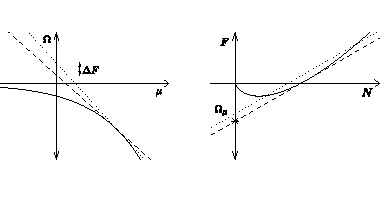
\includegraphics[scale=2.5]{img/Legender_transform.pdf}
  \caption{(a) Перетворення Лежандра, яке дає $F(N)$, відповідає опису кривої $\Omega\mu$ властивостями її дотичних: мінус їх нахили $N = -(\partial{\Omega}/\partial{\mu})$. та їх перетину з енергетичною віссю, $F = \Omega + \mu N$. Той факт, що похідна $\Delta F / \Delta N$ дорівнює $\mu$, слідує з формулювання питання: якщо дві сусідні прямі перетинають енергетичну вісь на відстані $\Delta F$ один від одного і мають нахили, які відрізняються на $\Delta N$, на якій відстані від осі вони будуть перетинати один одного? (b) Зворотне перетворення Лежандра з $F(N)$ в $\Omega (\mu)$ має аналогічну інтерпретацію. Мінімізація, запропонована в рівнянні. \ref{eqn:grand-potentialfunc} відповідає вивченню сімейства ліній з фіксованим нахилом $\mu$, які проходять через точки $N, F$ на кривій вільної енергії. Їх перетин, має мінімум (зазначений зірочкою) для тієї лінії, яка є дотичною до кривої \cite{Argaman_2000}.}
  \label{fig:legander_transform}
\end{figure}
\subsection{Підхід Кона-Шема}
Наведене вище обговорення можна досить просто узагальнити на обробку частинок у зовнішньому потенціалі $v(\textbf{r})$. Гамільтоніан багатьох тіл тепер дорівнює
\begin{equation}
\label{eqn:Ham}
	{\cal H}_{mb} = {\cal T} +{\cal V} +{\cal U},
\end{equation}
де ${\cal V} = \sum\limits_{i=0}^M v(\textbf{r}_i)$ -- потенційна енергія. Омега-потенціал і омега-функція були визначені як рів.\ref{eqn:omegapotential} та \ref{eqn:grand-potentialfunc}, але зараз вони залежать від потенціальної функції $v(\textbf{r})$, а не скалярного об'єму $V$. Тому $\Omega = \Omega(\mu, T, [v(\textbf{r})])$ тепер є функціоналом $v(\textbf{r})$, а тако ж функцією $\mu$ і $T$ -- квадратні дужки позначають функціональні змінні. 

Як добре відомо, потенціал $v(\textbf{r})$ - це енергія, яка вимірюється з довільного джерела, тобто Зміщення потенціалу на постійну величину не впливає на фізику системи. Тут зручно встановити цей початок координат в хімічному потенціалі, тобто прийняти $\mu = 0$. Еквівалентно, можна визначити нову функціональну змінну як $v(\textbf{r}) - \mu$, оскільки $\Omega$ залежить тільки від цієї різниці, а не від $v(\textbf{r})$ і $\mu$ окремо.

Функціональна похідна $\Omega$ за новою змінною дає розподіл щільності частинок, $n(\textbf{r}) = \langle \rho (\textbf{r}) \rangle$, де $\rho(\textbf{r}) = \sum\limits_{i=1}^M\delta(\textbf{r}-\textbf{r}_i)$ неперевірена щільність. Використовуючи (функціональне) перетворення Лежандра, як зазначено вище, ми можемо визначити нову вільну енергію, яка залежить від $n(\textbf{r})$, а не від $v(\textbf{r})$, і називається вільною енергією Хоенберга-Кона:
\begin{equation}
	\label{eqn:free_energ_hoenberg-khon}
	F_{HK}[n(\textbf{r})] = \Omega[v(\textbf{r})] - \int{n(\textbf{r}) v(\textbf{r})d\textbf{r}} 
\end{equation}
де зміною температури у явному вигляді ми знехтували і $v(\textbf{r)}$ з правої частини обрана так, щоб відповідати заданому $n(\textbf{r})$ (такий вибір можливий лише із-за загальної опуклості вільної енергії). Частина та функціональна похідна $F_{HK}[n(\textbf{r})]$ задається звичайним правилом перетворення Лежандра, як: $dF_{HK} = -SdT - \int{v(\textbf{r})\delta n(\textbf{r})d\textbf{r}}$.
Пряме узагальнення функції вильної енергії це і є функціонал вільної енергії:
\begin{equation}
	\label{eqn:free_energ_functional}
	\Omega[n(\textbf{r})] \equiv F_{HK}[n(\textbf{r})] + \int{n(\textbf{r})v(\textbf{r})d\textbf{r}}
\end{equation}
Якщо цей функціонал мінімізувати відносно $n(\textbf{r})$ і при постійному $v(\textbf{r})$ то функціонал вільної енергії дорівнює омега-потенціалу. Існування функціоналу $n(\textbf{r})$ з цією властивістю є одним з основних принципів DFT і є другою теоремою Хоенберга–Кона (див. наступний параграф).

Обговорення теореми Хоенберга-Кона, тим не менш, важливо навіть у введенні до DFT на основі перетворення Лежандра, оскільки процедура мінімізації вільної енергії, втілена в ньому, є центральною як для формування фізичної інтуїтивної картини DFT, так і для розробки ефективних чисельних схем для вирішення рівнянь DFT в практиці.

Узагальнюючи можна сказати, що в DFT Кона-Шема всі обмінні та кореляційні ефекти включені в обмінно-кореляційний функціонал $E_{xc}[n]$, котрий залежить від густини $n(\textbf{r})$ електронів. 


Функціонал повної енергії може бути записаний, як \cite{KSenergy}:
\begin{eqnarray}
 E[\psi_i] = 2\sum\limits_{i}\int\psi_i\left({{\hbar^2}\over{2m}}\right)\nabla^2\psi_id^3\textbf{r}+\int V_{ion}(\textbf{r})n(\textbf{r})d^3\textbf{r}+\nonumber \\
 {{e^2}\over{2}}\int {{n(\textbf{r})n(\textbf{r})}\over{|\textbf{r}-\textbf{r}^\prime|}}d^3\textbf{r}d^3\textbf{r}^\prime+E_{xc}[n(\textbf{r}^\prime)]+E_{ion}(R_i)
\end{eqnarray}

Де $V_{ion}$ -- повний електрон-іонний потенціал, $E_{xc}[n(\textbf{r}^\prime)]$ -- обмінно-кореляційний функціонал, $E_{ion}$ -- кулонівська енергія, $n(\textbf{r})$ -- електронна густина

\section{Теореми Кона-Шема}
Шляхом публікації двох статей Хохенбергом та Коном у 1964 році~\cite{Hohenberg&Khon}, а також Коном і Шемом в 1965 році~\cite{Khon&Sham}, в яких доводились теореми завдяки яким теорія функціоналу ґустини вийшла на новий рівень. Ці теореми встановлюють точну відповідність між електронною щільністю, зовнішнім потенціалом і хвильовою функцією.

\textbf{Перша теорема} говорить про те, що електронна щільність єдиним чином визначає оператор Гамільтона і, отже, всі характеристики системи.
Не можуть існувати два різні зовнішні потенціали, що призводять до однієї і тієї ж електронної щільності основного стану системи, іншими словами, електронна щільність основного стану однозначно визначається зовнішнім потенціалом.
Знаючи потенціал, ми знаємо Гамільтоніан системи, відповідно можемо знайти хвильову функцію системи та всі властивості системи, що визначаються електронною щільністю основного стану. Перша теорема показує зв'язок між зовнішнім потенціалом та електронною щільністю основного стану.

\textbf{Друга теорема} функціонал енергії, що визначає енергію квантового стану системи, визначає мінімальну енергію тоді і тільки тоді, коли електронна густина, що входить у функціонал, є реальною густиною основного квантового стану.
Таким чином, для знаходження точної енергії основного стану та його щільності, достатньо знати функціонал $E[n]$. Висновки цих теорем призводять до того, що для будь-якого зовнішнього потенціалу завжди можна знайти електронну густину та енергію основного стану, мінімізуючи цей функціонал.


\subsection{Самоузгоджене рівняння Кона-Шема}
Електронна щільність системи може бути знайдена з рішення самоузгодженого рівняння Кона-Шема, це випливає з наведених раніше теорем, яке можна записати так:

\begin{equation}
    \left[{{-\hbar^2}\over{2m}}\nabla^2+V_{ion}(\textbf{r})+V_H(\textbf{r})+V_{XC}(\textbf{r})\right]\psi_i(\textbf{r}) = e_i\psi_i(\textbf{r})
\end{equation}

Де $\psi_i$ -- хвильова функція стану $i$, $e_i$ -- власні значення, $V_H$ -- потенціал Хартирі, який відповідає за електронно-електронне відштовхування.

Явний вид обмінно-кореляційного потенціалу $V_{XC}$ ми не можемо знати принципово, тому його задають формально, функціональною похідною: 

\begin{equation}
    V_{XC} = \frac{\partial E_{XC}[n(\textbf{r})]}{\partial n(\textbf{r})}
\end{equation}

Для визначення об'ємно-кореляційного потенціалу використовують ряд наближень, про які ми поговоримо у наступному розділі.


\section{Методи апроксимації \textbf{$E_{xc}$}}
\subsection{LDA}
LDA (local density approximation) -- це клас наближень для обмінно-кореляційної енергії $E_{XC}$ у DFT, яка залежить виключно від електронної густини в кожній точці простору. Найуспішнішими локальними наближеннями є ті, що були отримані з моделі однорідного електронного газу (HEG)~\cite{Hohenberg&Khon}. 

Можна записати наступний вираз для обмінно-кореляційної енергії:

\begin{equation}
    E_{XC}^{LDA}[n(\textbf{r})] = \int{\epsilon_{xc}[n(\textbf{r})]n(\textbf{r})d^3\textbf{r}}
\end{equation}

Існує ряд параметрів для LDA, але ми їх не розглядатимемо.

\subsection{GGA}
GGA (generalized gradient approximations) -- на відміну від LDA в даний клас наближень включено градієнтну поправку для електронної щільності. Це усуває деякі недоліки LDA. Для узагальненого градієнтного наближення ми можемо записати, що $E_{xc}$ дорівнює деякій функції локальної щільності та її градієнта:

\begin{equation}
    E_{xc}^{GGA} = \int{\epsilon_{xc}[n(\textbf{r}),\nabla{n(\textbf{r})]n(\textbf{r})d^3\textbf{r}}}
\end{equation}

Найчастіше для розрахунків використовуються параметризації PBE (Perdew-Burke-Ernzerhof)~\cite{PBE} та PW91~\cite{PW91}.

\subsection{meta-GGA}
Фактично meta-GGA - це розширене наближення GGA. В яке, як вхідні дані, входить щільність позитивної орбітальної кінетичної енергії~\cite{Swapan&Gosh&Parr, Becke&Roussel, Tao&Perdew}.

У напівлокальному наближенні функціонал $E_{xc}$ зводиться до єдиного інтегралу загального вигляду:
\begin{equation}
    E_{XC}^{MGGA} = \int{\epsilon_{xc}[n(\textbf{r}),\nabla{n(\textbf{r}),\tau_{\sigma}(\textbf{r}})]}n(\textbf{r})d^3\textbf{r}
\end{equation}

Де $\tau_{\sigma}(\textbf{r})$ щільність кінетичної енергії зайнятих станів та визначається як:
\begin{equation}
    \tau_{\sigma}(\textbf{r}) = \sum\limits_{i\textbf{k}}|\nabla\psi_{i\textbf{k}}(\textbf{r})|^2
\end{equation}
\subsubsection{SCAN}
SCAN (Strongly-constrained and appropriately-normed) meta-GGA, раніше розроблені meta-GGA функціонали виявилися менш точними для розрахунку критичних тисків у структурно-фазових переходах твердих тіл, а також для матеріалів з шаруватою структурою відомі, як Ван-дер-Ваальсовські матеріали. SCAN покликаний усунути цю проблему за допомогою додавання в обмінно-кореляційний функціонал безрозмірну змінну.
$\alpha$~\cite{SCAN}:
\begin{equation}
    \alpha = (\tau - \tau^W)/\tau^{unif} > 0
    \label{eqn:alpha}
\end{equation}

Де $\tau^W = |\nabla{n(\textbf{r})}|^2/8n(\textbf{r})$ є одноорбітальною межею $\tau$ \newline та $\tau^{unif} = (3/10)(3\pi^2)^{2/3}n(\textbf{r})^{5/3}$ межа рівномірної щільності.

Відомо багато особливостей точного функціоналу $E_{xc}$. неемпіричні функціонали, побудовані для задоволення точних обмежень на цей функціонал щільності, надійні в широкому діапазоні систем (наприклад, атомів, молекул, твердих тіл і поверхонь), включаючи багато, які не схожі на ті, для яких ці функціонали були протестовані і підтверджені. У цьому розділі ми більш глибше розкриємо імплементацію функціоналу, який вперше задовольняє всім відомим можливим точним обмеженням \hyperref[lst:Constrains]{[Список 2.1]} і відповідним чином нормується в системах, для яких напівлокальні функціонали можуть бути точними або надзвичайно точними.

\begin{itemize}	
\label{lst:Constrains}
   \item Для обмінної енергії
   \begin{itemize}
     \item Негативність 
     \item Спінове масштабування
     \item Однорідне масштабування щільності
     \item Неоднорідне масштабування щільності
     \item Розширення градієнту четвертого порядку
     \item Жорстка межа для двохелектронних щільностей
   \end{itemize}
   \item Для кореляційної енергії
   \begin{itemize}
   	  \item Негативність
   	  \item Розширення градієнту другого порядку
   	  \item Рівномірне масштабування щільності до межі високої щільності
   	  \item Рівномірне масштабування щільності до межі низької щільності
   	  \item Нульова енергія кореляції для будь-якої одноелектронної спін-поляризованої щільності
   	  \item Нерівномірне масштабування щільності
   	  \item Масштабуємітсь розмірів системи
   	  \item Границя Ліба-Оксфорда
   	  \item Слабка залежність від відносної спінової поляризації в межі низької щільності
   	  \item Статичний лінійний відгук однорідного електронного газу
   	  \item Межа Ліба-Оксфорда для двох густин електронів
   	\end{itemize}
 \captionof{constrains}{Обмеження для обмінно-кореляційної енергії $E_{xc}$.}
 \end{itemize}

Запишемо кореляційну енергію $\epsilon_c$ на один електрон рів. \ref{eqn:e_c}. Також намалюємо фактор посилення \ $F_{xc}(r_s, \xi, s, a)$ в наближені низької густини $r_s \rightarrow \infty$ \ref{fig:F_factor}. Тут $\xi = (n_\uparrow - n_\downarrow)/(n_\uparrow + n_\downarrow)$ спін поляризація, $r_s = (4 \pi n/3)^{-1/3}$, і $s = {|\nabla{n}|}/{2(3\pi^2)^{-1/3}
\\ n^{4/3}}$, $\alpha$ -- безрозмірний параметр \ref{eqn:alpha}. 

Напівлокальний обмінно-кореляційний функціонал можна записати наступним чином (знехтуємо $\nabla \xi$ та припустимо що параметр $\alpha$ однаковий для спін-неполяризаційних густин $2n_\uparrow$ та $2n_\downarrow$):

\begin{equation}
	\label{eqn:semilocalexc}
	E_{xc}[n_{\uparrow},n_{\downarrow}] = \int{d^3 r n\epsilon_{xc} = \int d^3 r n \epsilon_{x}(n)F(r_s,\xi, s, a)}
\end{equation}

Де $\epsilon_x^{unif} = -(3/4\pi)(3\pi^2n)^{1/3}$ обмінна енергія на електрон однорідного електронного газу.  
Кореляційну частину можна записати як: 

\begin{equation}
	\label{eqn:cor}
	E_{c}[n_{\uparrow},n_{\downarrow}] = \int{d^3 n \epsilon_c (r_s,\xi, s, a)}
\end{equation}

SCAN $\epsilon_c$ має наступну форму:

\begin{equation}
	\label{eqn:e_c}
	\epsilon_c = \epsilon_c^1 + f_c(\alpha)(\epsilon_c^0 -\epsilon_c^1)
\end{equation}

Де $f_c(a) = exp[-c_{1c}\alpha/(1-\alpha)]\theta(1-\alpha)-d_c exp[c_{2c}/(1-\alpha)]\theta(\alpha-1)$

У статі \cite{SCAN} переглядають форму PBE функціоналу для більш точного підходу до 2D межі при нерівномірному масштабуванні: 
\begin{equation}
	\epsilon_c^1 = \epsilon_c^{LSDA1}+H_1
\end{equation}

Де

\begin{equation}
	\label{eqn:H_1}
	H_1 = \gamma\phi^3ln[1+w_1(1-g(At^2))],
\end{equation}

\begin{equation}
	t = (3\pi^2/16)^{1/3}s/(\phi r_s^{1/2}),
\end{equation}

\begin{equation}
	w_1 = exp[-e_c^{LSDA1}/(\gamma\phi^3)] - 1,
\end{equation}

\begin{equation}
	A = \beta(r_s)/(\gamma w_1),
\end{equation}

\begin{equation}
	g(At^2) = 1 / (1 + 4At^2)^{1/4}.
\end{equation}

$\epsilon_c^{LSDA1}$ кореляційна енергія однорідного електронного газу. Тут використовується PW92 LSDA параметризація \cite{PhysRevB.45}. Де $\gamma = 0.0391091$, $\beta(r_s) = 0.066725(1 + 0.1r_s)/(1 + 0.1778r_s)$ \cite{PhysRevLett.103}, та $\phi = [(1 + \xi)^{2/3} + (1 - \xi)^{2/3}]/2$. $\epsilon_c^1$ відрізняється від оригінальної PBE кореляції тільки в виразах для $\beta(r_s)$ та $g(At^2)$. Оригінальна кореляційна енергія з PBE  функціоналу \cite{PBE} має для цих виразів наступні значення $\beta(r_s) = 0.066725$ та $g(At^2) = 1 / (1 + At^2 + A^2 t^4)$.

Таким чином можна надати вигляд $\epsilon_c^0$ за аналогією до $\epsilon_c^1$, реалізація цього відбувається за умови, що для $\alpha = 0$ може виникнути зміна градієнту густини s:
\begin{equation}
	\epsilon_c^0 = (e_c^{LDA0} + H_0) G_c(\xi),
\end{equation}

Де 

\begin{equation}
	\label{eqn:G_c}
	G_c(\xi) = \big\{1 - 2.3631[d_x(\xi) - 1]\big\} (1 - \xi^12), 
\end{equation}

\begin{equation}
	d_x(\xi) = [(1+\xi)^{4/3} + (1 - \xi)^4/3] / 2,
\end{equation}

\begin{equation}
	\epsilon_c^{LDA0} = -b_{1c}/(1+b_{2c}r_s^{1/2}+b_{3c}r_s)
\end{equation}

Вираз $G_c(\xi)$ \ref{eqn:G_c} був спроєктований щоб кореляційна енергія зверталася в нуль для будь-якої електронної щільності та зробити $F_{xc}(r_s \rightarrow \infty, \xi, s = 0, \alpha = 0)$ незалежним від $\xi$ для $0 \leq |\xi| < 0.7$. Точна обміно-кореляційна енергія в межі низької щільності не залежить від $\xi$. Це здобувається за допомогою s = 0 точно у $\alpha = 0$ і як можна краще у $\alpha = 0$. 

Аналогічно до $H_1$ \ref{eqn:H_1}, 

\begin{equation}
	H_0 = b_{1c}ln[1+w_0(1 - g_\infty(\xi = 0, s))], 
\end{equation} 

Де 
\begin{equation}
	w_0 = exp[-e_c^{LDA0}/b_{1c}]-1,
\end{equation}
\begin{equation}
	g_\infty(\xi,s) = \lim_{r_s \rightarrow \infty}g(At^2) = 1 / (1 + 4\chi_\infty s^2)^{1/4}.
\end{equation}
Де $\chi_\infty(\xi) = \left(\frac{3\pi^2}{16}\right)^{\frac{2}{3}}\beta(r_s \rightarrow \infty)\phi/[c_x(\xi)-f_0]$, $c_x(\xi) = -(3/4\pi)(9\pi/4)^{1/3}d_x(\xi)$, $f_0 = -0.9$. При $\xi = 0$, $ \chi_\infty(\xi = 0) = 0.128026$.

Параметри $b_{1c} = 0.0285764$, $b_{2c} = 0.0889$, $b_{3c} = 0.125541$, визначаються у наступній процедурі:

У межі великої густини, $e_c^0 = b_{1c}G_c(\xi)ln\{1 - g_\infty(\xi = 0, s)exp(1)/[exp(1)+1]\}$ та $b_{1c} = 0.0285764$ за допомогою підгонки до кореляційної енергії $E_c = -0.0467 Ha$ високої густини двохелектронного іону з атомним номером $Z \rightarrow \infty$. $b_{3c} = 0.125541$ визначається нижчою межею обмінно-кореляційних енергій двохелектронної системи, $F_{xc} \leq 1.67082$. $b_{2c} = 0.0889$ підганяється до $E_{xc}(He) = -1.068 Ha$. Параметри у інтерполяційної/екстраполяційної функції наступні $c_{1c} = 0.64, c_{2c} = 1.5, d_c = 0.7$.

Сім параметрів ($c_{1x}, c_{2x}, d_x, k_1, c_{1c}, c_{2c}, d_c$) можна визначити наступним чином: для заданого $k_1$, ми підганяємо до 
\begin{enumerate}
    \item $\gamma_{x1} = -0.2259$, $\gamma_{x2} = 0.2551$, $\gamma_{c1} = 0.0388$ асимптотичні коефіцієнти великого Z для обміну і кореляції атомів рідкісних газів з атомним номером Z,
    \item Крива енергії зв'язку стисненого Ar$_2$ (із середньою абсолютною похибкою менше 1 ккал / моль для довжин зв'язків R=1.6, та 2.0 $\angstrom$),
    \item обмінно-кореляційна енергія поверхні желе при параметрі насипної щільності $r_s = 4 \ Bohr$ в межах 5\% від значення QMC \cite{PhysRevB.76}.
\end{enumerate}

Потім обирається набір параметрів з максимальним значенням $k_1$, оскільки точні енергії обміну для модельних густин металів з посилання \cite{PhysRevB.54} припускають, що $k_1$ не повинен бути занадто маленьким.

Для повноти, нарешті, можна навести розкладання градієнта четвертого порядку для енергії обміну, яке діє у наступному інтервалі $0 \leq s \ll 1$ та $a \approx 1:$

\begin{eqnarray}
	F_x^{GE4}(s,a) = 1+(10/81)s^2 - (1606/18225)s^4 +\nonumber \\
 + (511/13500)s^2(1-\alpha) + (5913/405000)(1-\alpha)^2.      
\end{eqnarray}

SCAN дуже добре пророкує певні властивості зв'язку: енергію атомізації, енергії зв'язку при слабкій взаємодії і константи решітки твердих тіл, але не енергетичні бар'єри для хімічних реакцій. Ми припускаємо, що перші три властивості природним чином потрапляють в область хорошого напівлокального функціоналу, в той час як четверте вимагає повністю нелокальної апроксимації (наприклад, корекція самовзоємодії для SCAN).
 
\begin{figure}[H]
\centering
\label{fig:F_factor}
	\begin{subfigure}{.9\textwidth}
		\hspace*{-1.2cm}
    	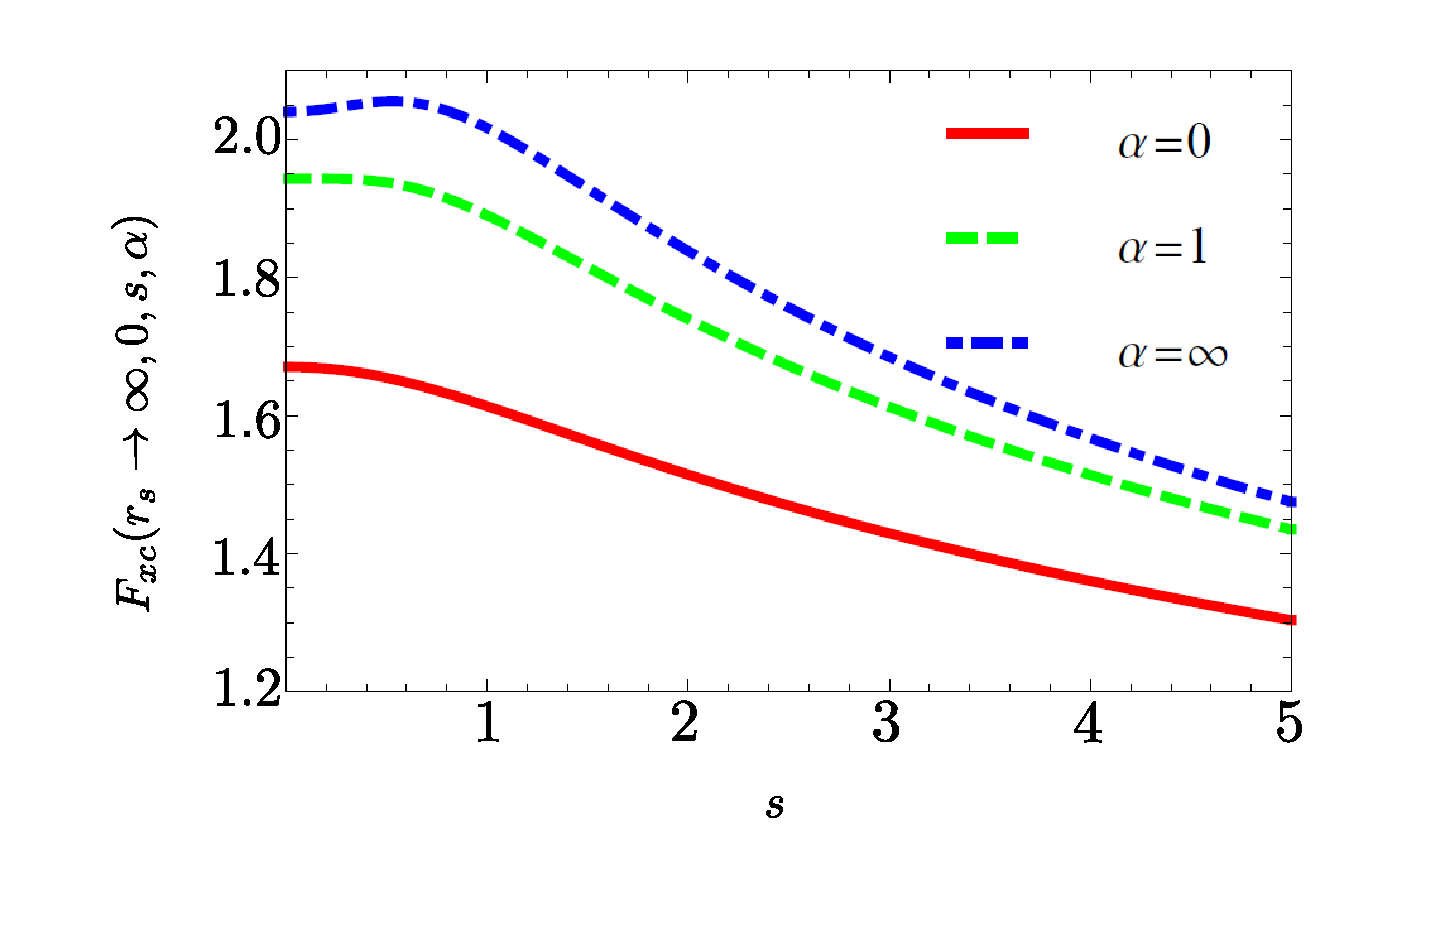
\includegraphics[width=1.0\linewidth]{F_factor1v3.pdf}
    	\caption{Фактор посилення обмінної кореляції в межі низької густини для спін-неполяризованого випадку.}
    	\label{fig:sub1}	
	\end{subfigure}
	
	\begin{subfigure}{.9\textwidth}
		\hspace*{0.15cm}
    	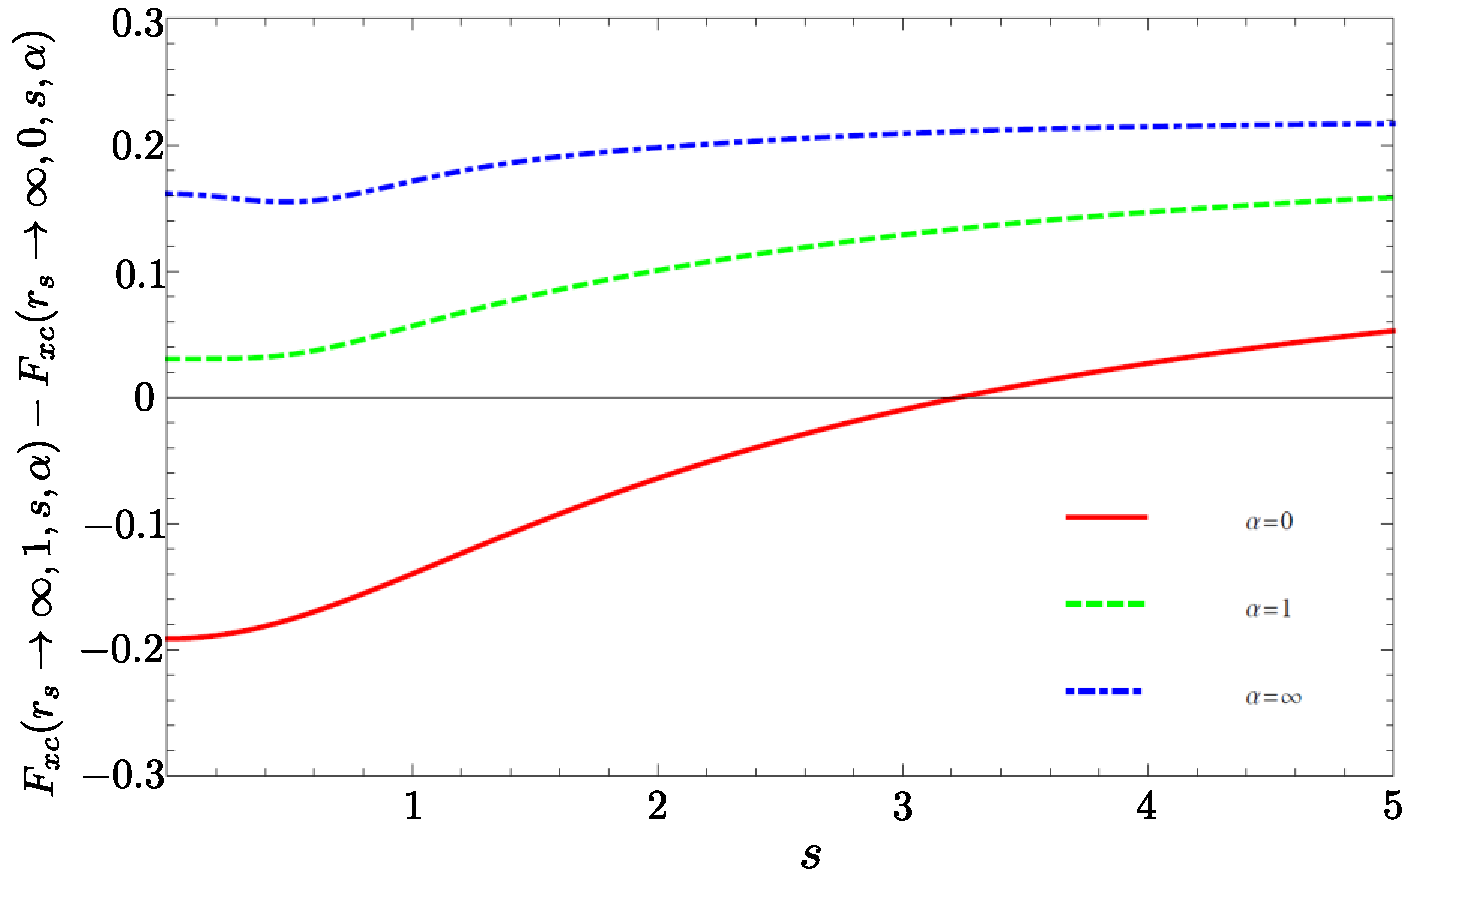
\includegraphics[width=1.0\linewidth]{F_factor2.pdf}
    	\caption{
    	Різниця між повністю спін-поляризованим ($\xi = 1$) і неполяризованим ($\xi = 0$) фактором посилення обмінної кореляції в межі низьких густин ($r_s \rightarrow \infty$).}
    	\label{fig:sub1}	
	\end{subfigure}
\caption{Фактор посилення при низькій щільності градієнту.}
\end{figure}

\section{Взаємодія Хаббарда: DFT + U}
Багато з найцікавіших проблем фізики конденсованих середовищ пов'язані з матеріалами, в яких електрони мають тенденцію локалізуватися і сильно взаємодіяти, такими як оксиди перехідних металів і рідкісноземельні елементи, а також сполуки, які частково займають $d$ і $f$ стану. Звичайні функціонали, такі як LDA і GGA, виявляють, що система являє собою метал, але насправді це магнітний ізолятор. Навіть якщо енергія основного стану визначена правильно, то зонні спектри сильно можуть відрізнятися від того, що ми бачимо в експерименті. Фундаментальна проблема полягає у тому що не існує унікального шляху для визначення локальних орбіталей. 

Абревіатура "LDA+U" часто використовується для позначення методів, які включають обчислення типу LDA або GGA в поєднанні з додатковою орбітально-залежною взаємодією \cite{PhysRevB.44, Anisimov1997}, але в цій роботі використовується більш загальний термін "DFT+U." додаткова взаємодія зазвичай розглядається тільки для високолокалізованих атомно-подібних взаємодій, орбіталі на тій же ділянці, тобто тієї ж форми, що і взаємодія "U" в моделях Хаббарда. Ефект доданого члена полягає в зміщенні локалізованих орбіталей відносно інших орбіталей, що намагається виправити помилки, які, як відомо, є великими в звичайних обчисленнях LDA або GGA. Наприклад, енергії просування в атомах перехідних металів ілюструють той факт, що відносні енергії зміщуються в залежності від наближення для обміну. Інший ефект виникає в частково заповнених $d$ і $f$ станах, де заняття однієї орбіталі підвищує енергію інших орбіталей, в результаті чого це сприяє магнітним станам. Оскільки ефекти мають вирішальне значення для багатьох завдань, пов'язаних з $3d$ оксидами перехідних металів та іншими матеріалами, розрахунки "DFT+U" є невід'ємною частиною сучасних методів.

Багато прикладів обчислень "DFT+U" наведені в \cite{Anisimov1997}. Прототипними прикладами є оксиди перехідних металів. Можливо, найбільш відомими прикладами є вихідні сполуки надпровідників CuO, які, як виявилося, є немагнітними металами в звичайних розрахунках LDA і GGA, тоді як розрахунки "DFT+U" знаходять правильне рішення для антиферомагнітного ізолятора \cite{Anisimov1997}. Звичайна теорія спінової щільності для таких матеріалів, як MnO та NiO, знаходить правильні спінові стани і енергетичну щілину, але величина щілини занадто мала, як показано на рис. \ref{fig:GAP}. Розрив набагато краще з гібридними функціоналами; однак часто простіше і інтуїтивно зрозуміліше виправити розрив за допомогою члена "U", який збільшує розрив між заповненим і порожнім $3d$-станами і здвигає стани до станів кисню, щоб вони набагато краще узгоджувалися з експериментом.

\begin{figure}[H]
	\centering
	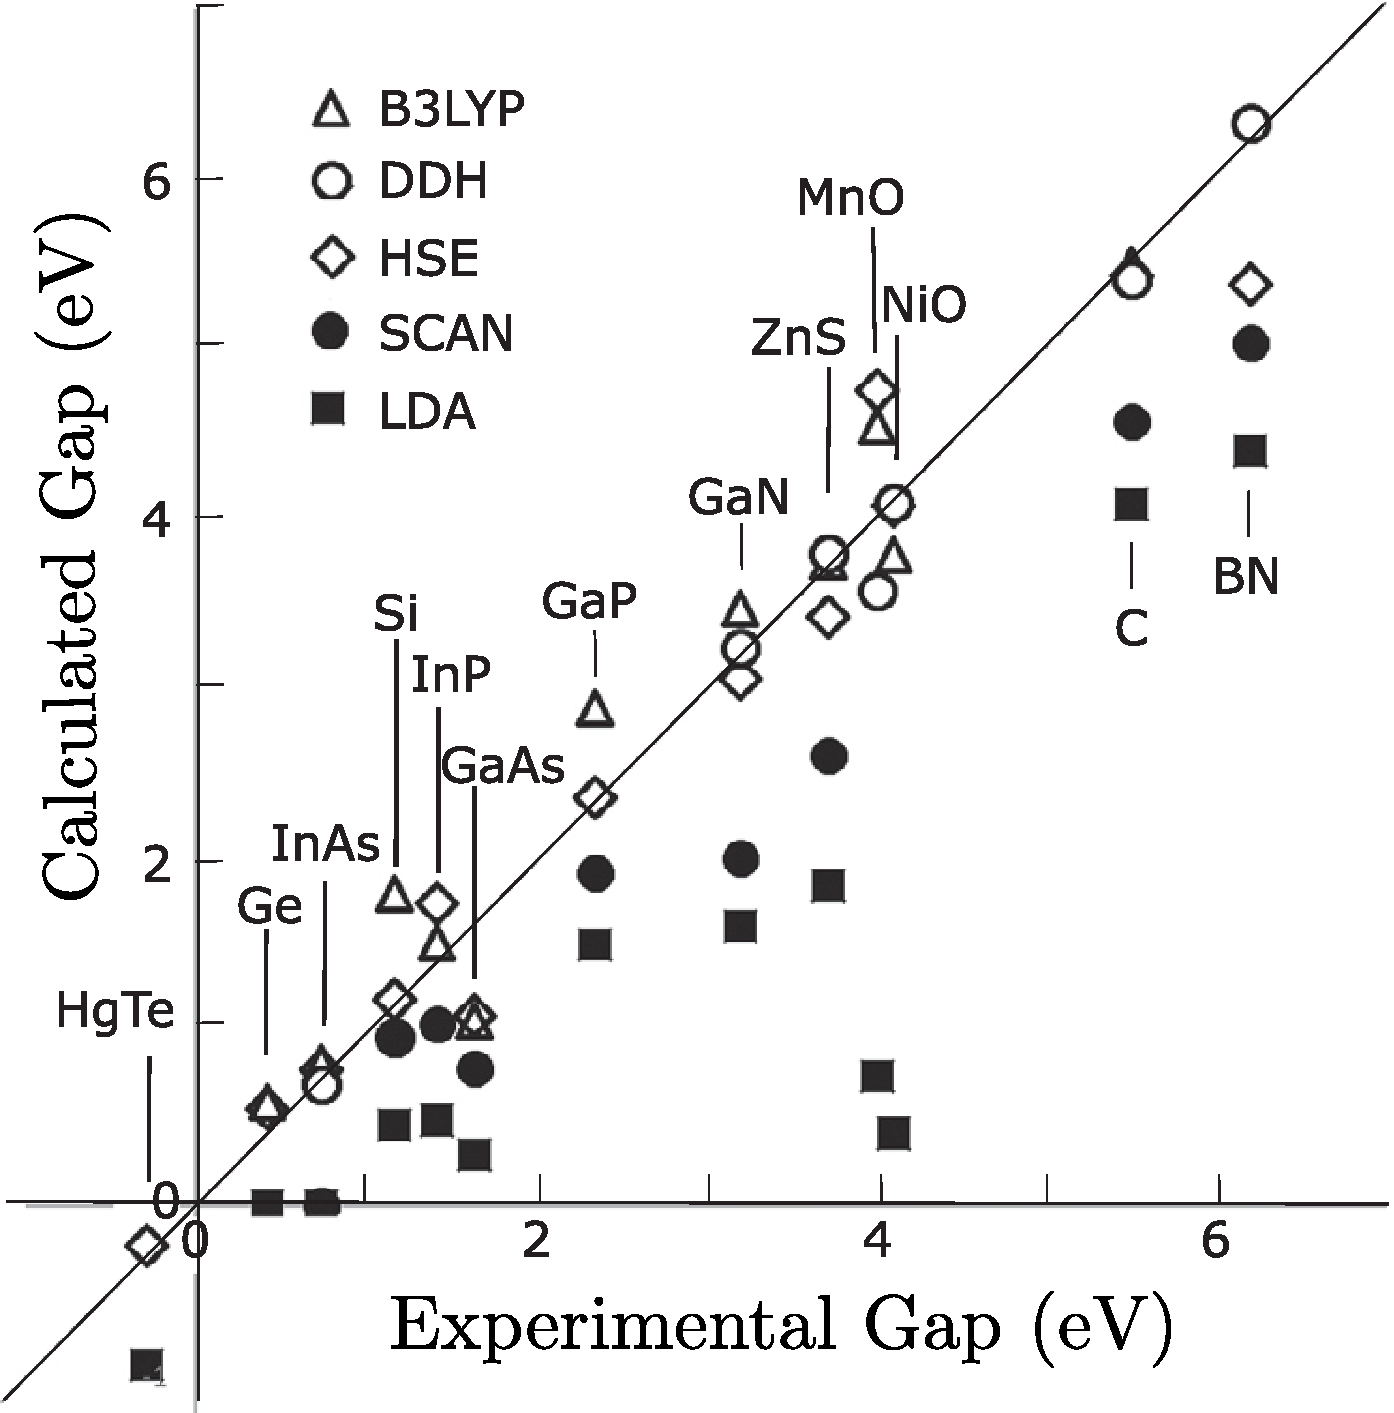
\includegraphics[scale=0.5]{GAP.pdf}
	\caption{Заборонені зони в порівнянні з експериментом для різних функціоналів. Функціонали LDA і meta-GGA позначаються закритими символами, а гібридні функціонали - відкритими символами. В цілому, гібридні функціонали набагато краще підходять для прогалин, але вони вимагають значно більших обчислювальних зусиль.}
	\label{fig:GAP}
\end{figure}

\section{Висновки до розділу}
У даному розділі був зроблен короткий вступ до Теорії Функціоналу Густини та огляд існуючих апроксимацій обміно-кореляційного потенціалу $E_{xc}$ (поза обговоренням залишись гібридні функціонали).
Енергія основного стану, електронна щільність і пов'язані з ними властивості звичайної матерії можуть бути ефективно обчислені, коли обмінно-кореляційна енергія як функціонал щільності апроксимується напівлокально. В даній роботі запропоновано мета-GGA (мета-узагальнену градієнтну апроксимацію), яка повністю обмежена, підкоряючись всім 17 відомим точним обмеженням. Він також точний або майже точний для набору відповідних норм, включаючи атоми рідкісних газів і незв'язані взаємодії. SCAN meta-GGA забезпечує чудову точність для систем, в яких точна обмінно-кореляційна дірка локалізована поблизу її електрона, і особливо для постійних решітки і слабких взаємодій.

Для описання досліджуваних систем був обраний SCAN функціонал з додаванням Хаббардовської взаємодії. З тих причин, що SCAN не достатньо все ж таки точний, щоб описувати сильнокорельовані системи.





\chapter{Аналіз отриманих результатів}
\section{Структурні дані та метод розрахунку}
Як вже було зазначено у вступній частині. Шарувата структура MX$_2$ утворена площинами, що складаються з одного шару атомів M (метал), який знаходиться між двома шарами атомів X (халькоген). Проміжний шар з'єднаний за допомогою сили Ван-дер-Ваальса. Атомна структура шаруватого MX$_2$ показана на рис. \ref{structure} \cite{FU2016221}, (\textbf{b}) показує решітку зверху, підкреслюючи порушення інверсійної симетрії. 

\begin{figure}
	\centering
	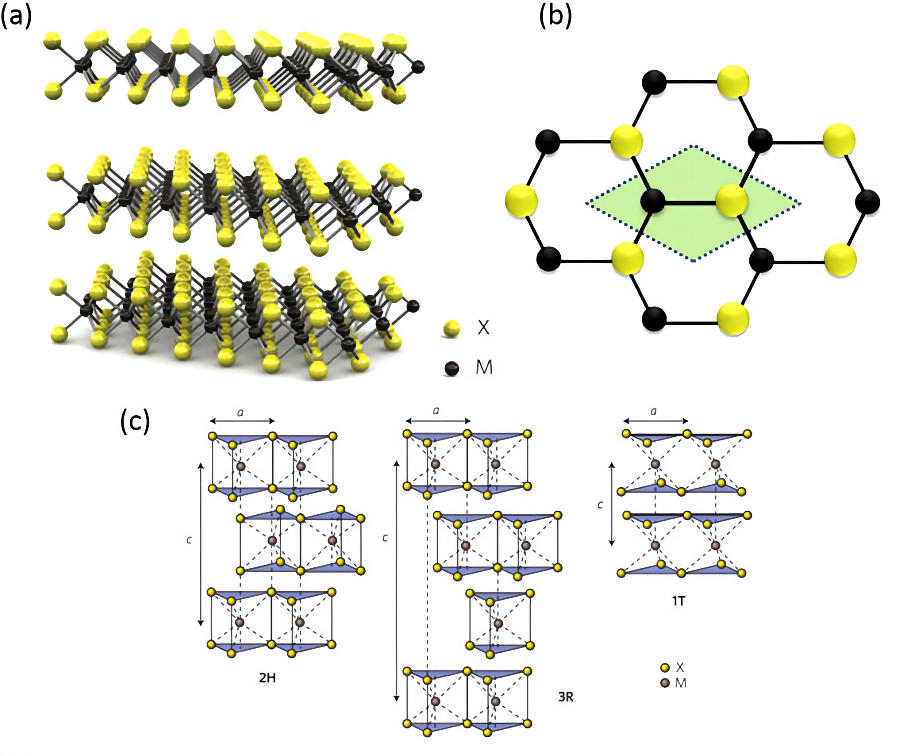
\includegraphics[scale=1]{structure.pdf}
	\caption{(а) тривимірна принципова схема атомної структури шаруватого MX$_2$, атоми металу (M) виділені чорним кольором, а атоми халькогену (X) - жовтим. (b) вид зверху решітки MX$_2$, що підкреслює порушення інверсійної симетрії. (c) схеми структурних політипів. Існує три структурних політипу багатошарової структури MX2: 2H, 3R і 1T з міжшаровим відстанню $\approx$ 0,7 нм.}
	\label{structure}
\end{figure}

У рамках даної роботи вивчалась саме 1T структура. У таблиці \ref{tab:Structure} наведено структурні дані ґратки, які отримані експериментально за допомогою методу рентгенівського дифракційного аналізу.

\begin{table}[!htp]\centering

\scriptsize
\begin{tabular}{lrrrrrrrrrrr}\toprule
\multicolumn{3}{c}{\textbf{TiS$_2$}} & &\multicolumn{3}{c}{\textbf{TiSe$_2$}} & &\multicolumn{3}{c}{\textbf{TiTe$_2$}} \\\midrule
\textbf{a} &\textbf{b} &\textbf{c} & &\textbf{a} &\textbf{b} &\textbf{c} & &\textbf{a} &\textbf{b} &\textbf{c} \\
3.407000 &3.407000 &5.695000 & &3.540000 &3.540000 &6.010000 & &3.768000 &3.768000 &6.460000 \\
\textbf{$\alpha$} &\textbf{$\beta$} &\textbf{$\gamma$} & &\textbf{$\alpha$} &\textbf{$\beta$} &\textbf{$\gamma$} & &\textbf{$\alpha$} &\textbf{$\beta$} &\textbf{$\gamma$} \\
90.000000 &90.000000 &119.999996 & &90.000000 &90.000000 &119.999999 & &90.000000 &90.000000 &119.999998 \\
\textbf{x} &\textbf{y} &\textbf{z} & &\textbf{x} &\textbf{y} &\textbf{z} & &\textbf{x} &\textbf{y} &\textbf{z} \\
0.000000 &0.000000 &0.000000 & &0.000000 &0.000000 &0.000000 & &0.000000 &0.000000 &0.000000 \\
0.333330 &0.666670 &0.749900 & &0.333330 &0.666670 &0.250000 & &0.333330 &0.666670 &0.250000 \\
0.666660 &0.333330 &0.250100 & &0.666660 &0.333330 &0.750000 & &0.666660 &0.333330 &0.750000 \\
\bottomrule
\end{tabular}
\caption{Координати атомів, постійні ґраток та кути TiS$_2$, TiSe$_2$, TiTe$_2$.}\label{tab:Structure}
\end{table}

Розрахунок робився за допомогою програмного пакету VASP (Vienna Ab initio Simulation Package) \cite{VASP1,VASP2, VASP3, VASP4} з PAW методом. Енергія плоских хвиль була в межах до 400 eV та 24 $\times$ 24 $\times$ 12 для розрахунку DOS. Для зонного розрахунку використовувались ті самі значення енергій для плоских хвиль та наступний к-шлях: $\Gamma-M-K-\Gamma-A-L-H-A$.
Вся постоброка відбувалась за допомогою Python 3 \cite{Python} та бібліотек для аналізу DFT розрахунків Pymatgen \cite{PyMatgen}, IFermi \cite{Ifermi}. 

В цілому електронна будова TiS$_2$, TiTe$_2$ та TiSe$_2$ має схожий вигляд. Зона провідності складається з $d$ орбіталей металу, а верх валентної зони складається з $p$ орбіталей і вони перетинаються у точці $L$ для TiS$_2$, $L$ та $M$ у TiSe$_2$, TiTe$_2$. 

Методологія була наступною, спочатку були отримані дані за допомогою звичайного GGA функціоналу у PBE параметризації для порівняння зі SCAN-ом, а саме, наскільки SCAN більш адекватно описує матеріал після структурної релаксації таб. \ref{tab:GGAlat}, таб. \ref{tab:SCANlat}. Та остаточно визначити щілину додавши поправки rVV10, які беруть до уваги взаємодію ван-дер-Ваальса.

\begin{table}[!htp]\centering
\scriptsize
\begin{tabular}{lrrrrrrr}\toprule
\multicolumn{7}{c}{\textbf{GGA}} \\\midrule
\multicolumn{3}{c}{\textbf{Оптимізована струкута}} & &\multicolumn{3}{c}{\textbf{\%}} \\
\multicolumn{7}{c}{\textbf{TiS$_2$}} \\
\textbf{a} &\textbf{b} &\textbf{c} & &\textbf{a} &\textbf{b} &\textbf{c} \\
3.412015 &3.412013 &6.446000 & &0.147089 &0.147030 &12.371304 \\
\textbf{$\alpha$} &\textbf{$\beta$} &\textbf{$\gamma$} & &\textbf{$\alpha$} &\textbf{$\beta$} &\textbf{$\gamma$} \\
89.999997 &90.000022 &119.999994 & &-0.000003 &0.000024 &-0.000002 \\
\multicolumn{7}{c}{\textbf{TiSe$_2$}} \\
\textbf{a} &\textbf{b} &\textbf{c} & &\textbf{a} &\textbf{b} &\textbf{c} \\
3.541846 &3.541879 &6.603517 & &0.052133 &0.053065 &9.410809 \\
\textbf{$\alpha$} &\textbf{$\beta$} &\textbf{$\gamma$} & &\textbf{$\alpha$} &\textbf{$\beta$} &\textbf{$\gamma$} \\
89.998535 &90.000481 &119.999714 & &-0.001628 &0.000534 &-0.000238 \\
\multicolumn{7}{c}{\textbf{TiTe$_2$}} \\
\textbf{a} &\textbf{b} &\textbf{c} & &\textbf{a} &\textbf{b} &\textbf{c} \\
3.766554 &3.766586 &6.865603 & &-0.038383 &-0.037534 &6.087574 \\
\textbf{$\alpha$} &\textbf{$\beta$} &\textbf{$\gamma$} & &\textbf{$\alpha$} &\textbf{$\beta$} &\textbf{$\gamma$} \\
89.998136 &90.001023 &119.998697 & &-0.002071 &0.001137 &-0.001084 \\
\bottomrule
\end{tabular}
\caption{Відхилення оптимізованої структури від експериментальної за допомогою GGA.}\label{tab:GGAlat}
\end{table}


\begin{table}[!htp]\centering
\scriptsize
\begin{tabular}{lrrrrrrr}\toprule
\multicolumn{7}{c}{\textbf{SCAN}} \\\midrule
\multicolumn{3}{c}{\textbf{Оптимізована струкута}} & &\multicolumn{3}{c}{\textbf{\%}} \\
\multicolumn{7}{c}{\textbf{TiS$_2$}} \\
\textbf{a} &\textbf{b} &\textbf{c} & &\textbf{a} &\textbf{b} &\textbf{c} \\
3.421272 &3.421262 &5.890012 & &0.418027 &0.417734 &3.366626 \\
\textbf{$\alpha$} &\textbf{$\beta$} &\textbf{$\gamma$} & &\textbf{$\alpha$} &\textbf{$\beta$} &\textbf{$\gamma$} \\
90.003098 &89.996423 &120.010782 & &0.003442 &-0.003975 &0.008988 \\
\multicolumn{7}{c}{\textbf{TiSe$_2$}} \\
\textbf{a} &\textbf{b} &\textbf{c} & &\textbf{a} &\textbf{b} &\textbf{c} \\
3.546469 &3.546465 &6.283398 & &0.182573 &0.182461 &4.447883 \\
\textbf{$\alpha$} &\textbf{$\beta$} &\textbf{$\gamma$} & &\textbf{$\alpha$} &\textbf{$\beta$} &\textbf{$\gamma$} \\
90.001939 &89.998709 &119.992066 & &0.002154 &-0.001434 &-0.006611 \\
\multicolumn{7}{c}{\textbf{TiTe$_2$}} \\
\textbf{a} &\textbf{b} &\textbf{c} & &\textbf{a} &\textbf{b} &\textbf{c} \\
3.758144 &3.758125 &6.857830 & &-0.261914 &-0.262419 &5.974397 \\
\textbf{$\alpha$} &\textbf{$\beta$} &\textbf{$\gamma$} & &\textbf{$\alpha$} &\textbf{$\beta$} &\textbf{$\gamma$} \\
89.992373 &90.008670 &119.993283 & &-0.008475 &0.009633 &-0.005596 \\
\bottomrule
\end{tabular}
\caption{Відхилення оптимізованої структури від експериментальної за допомогою SCAN.}\label{tab:SCANlat}
\end{table}

\clearpage
\begin{figure}[H]
\centering
	\begin{subfigure}[b]{.9\textwidth}
    	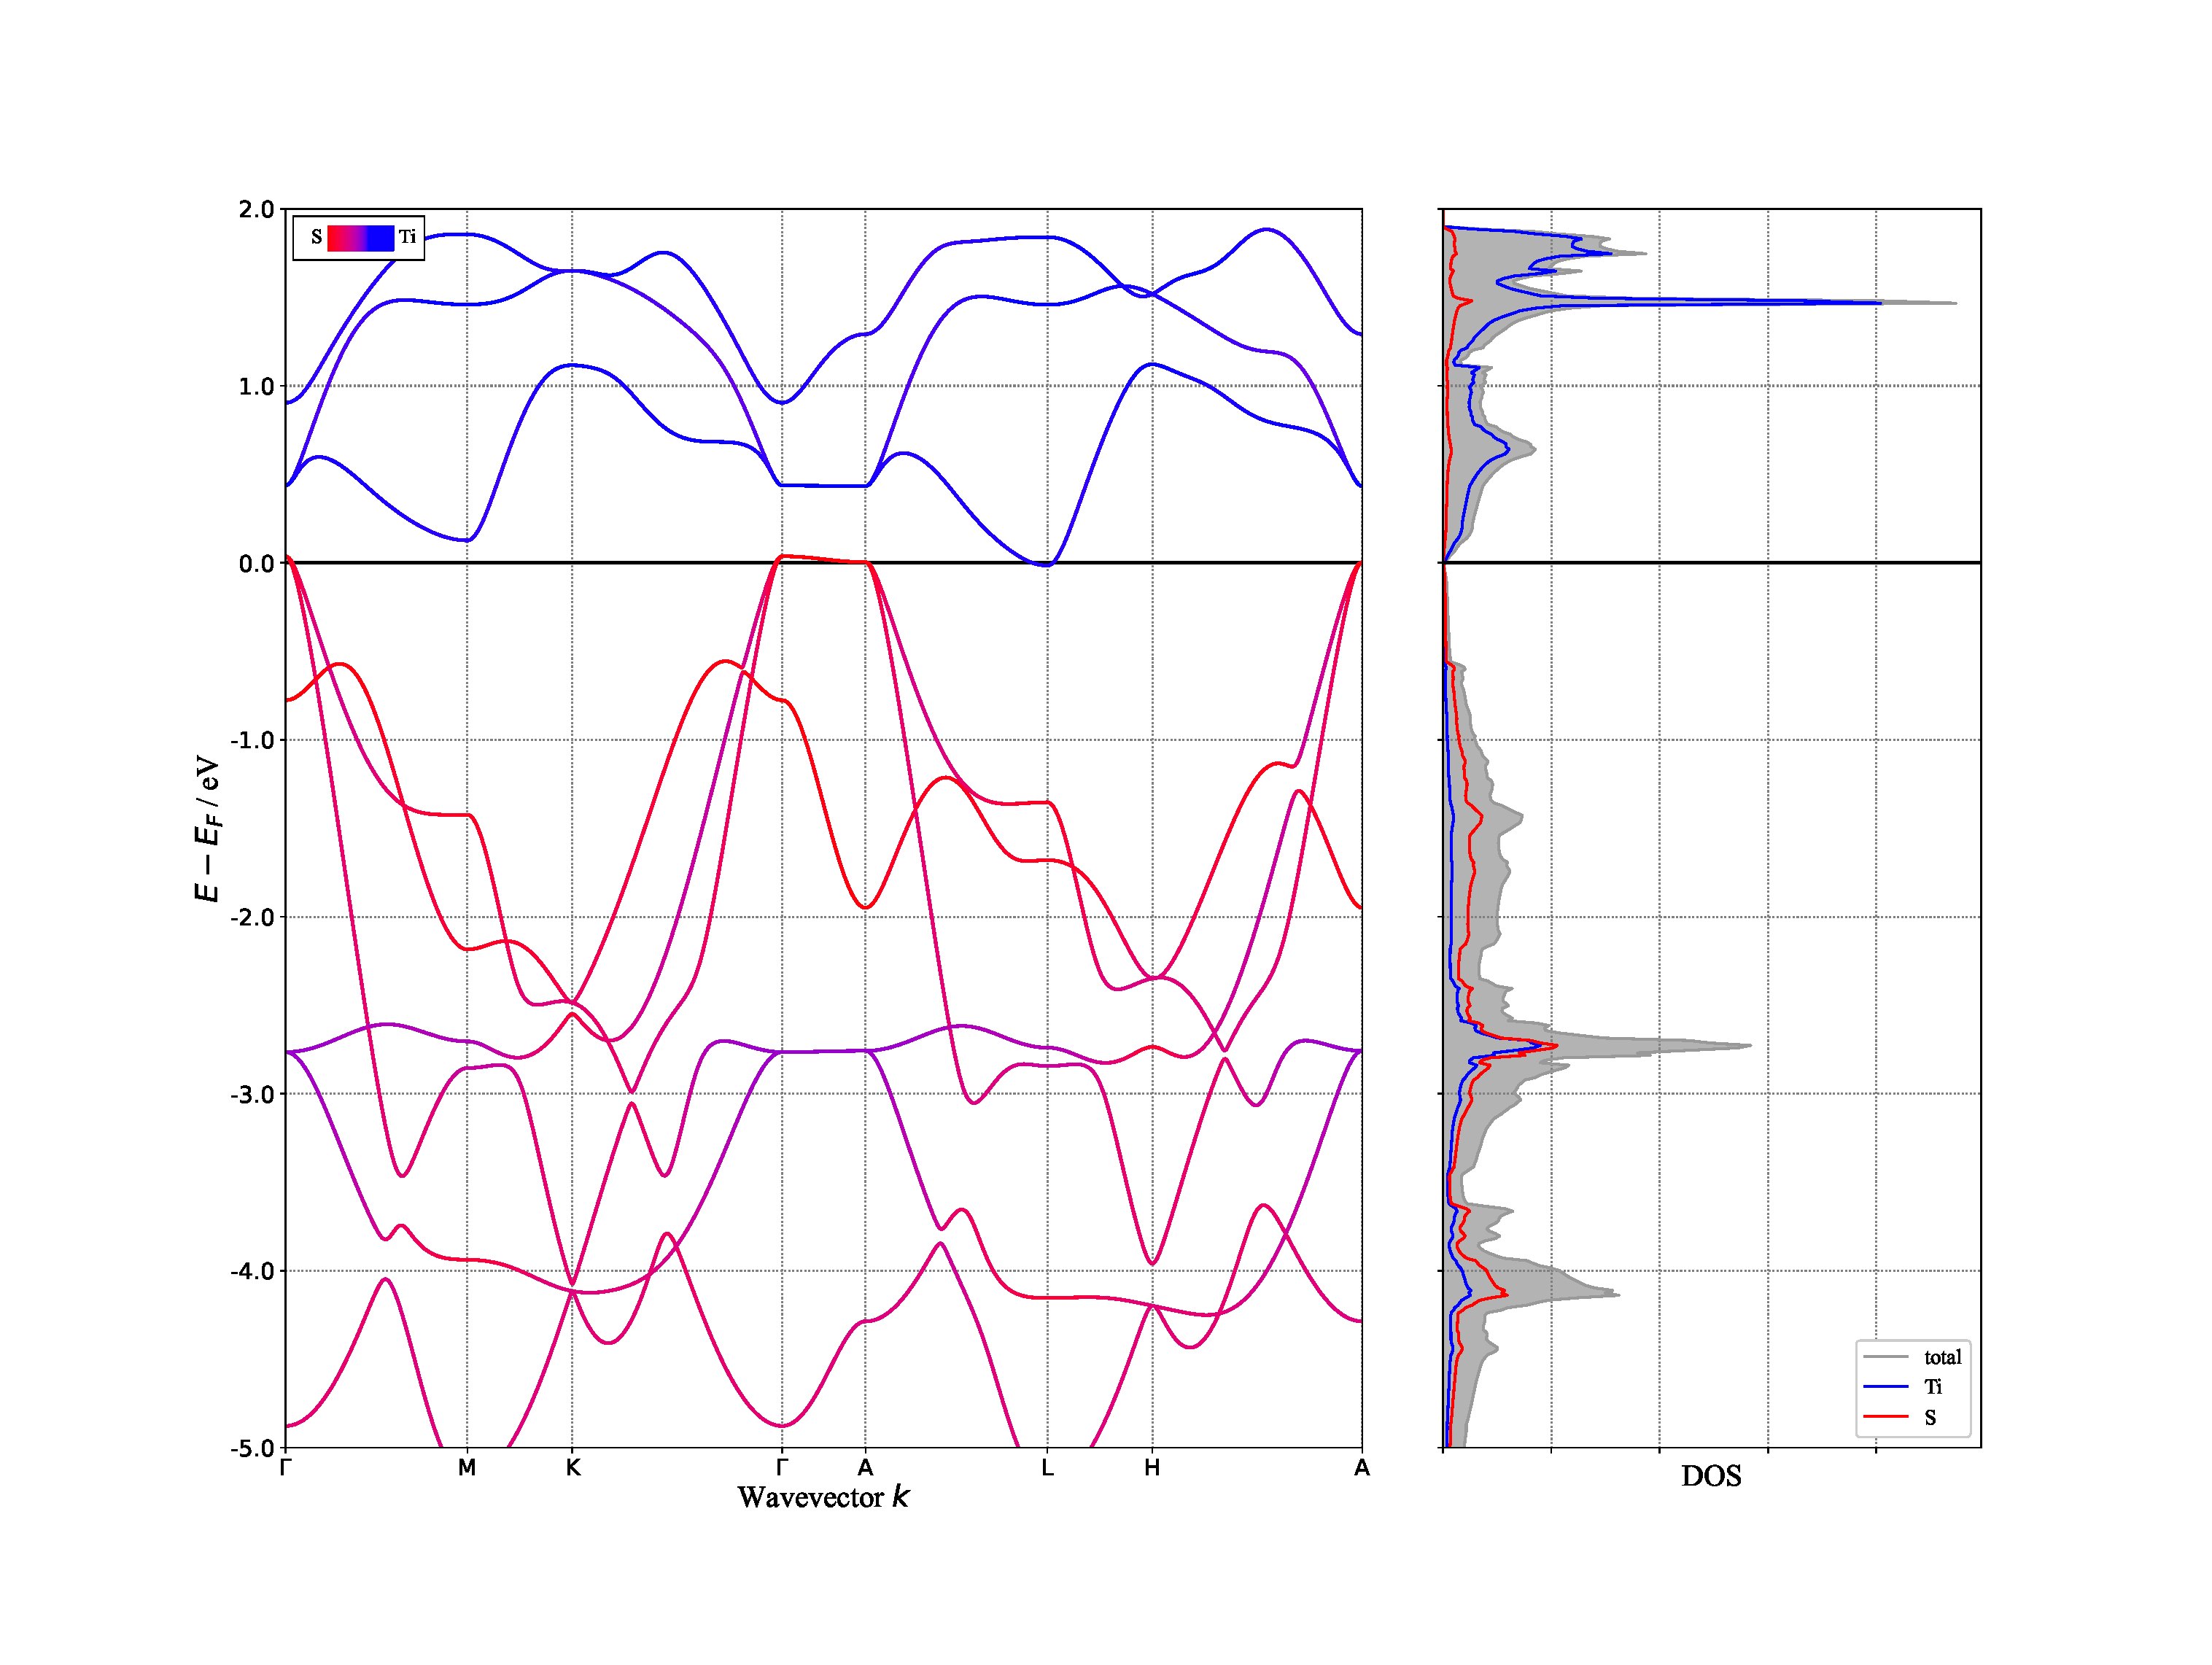
\includegraphics[width=\linewidth]{img/results/TiS2_GGA_relaxed_BAND+DOS.eps}
    	\caption{TiS2}
	\end{subfigure}
	\begin{subfigure}[b]{.4\textwidth}
    	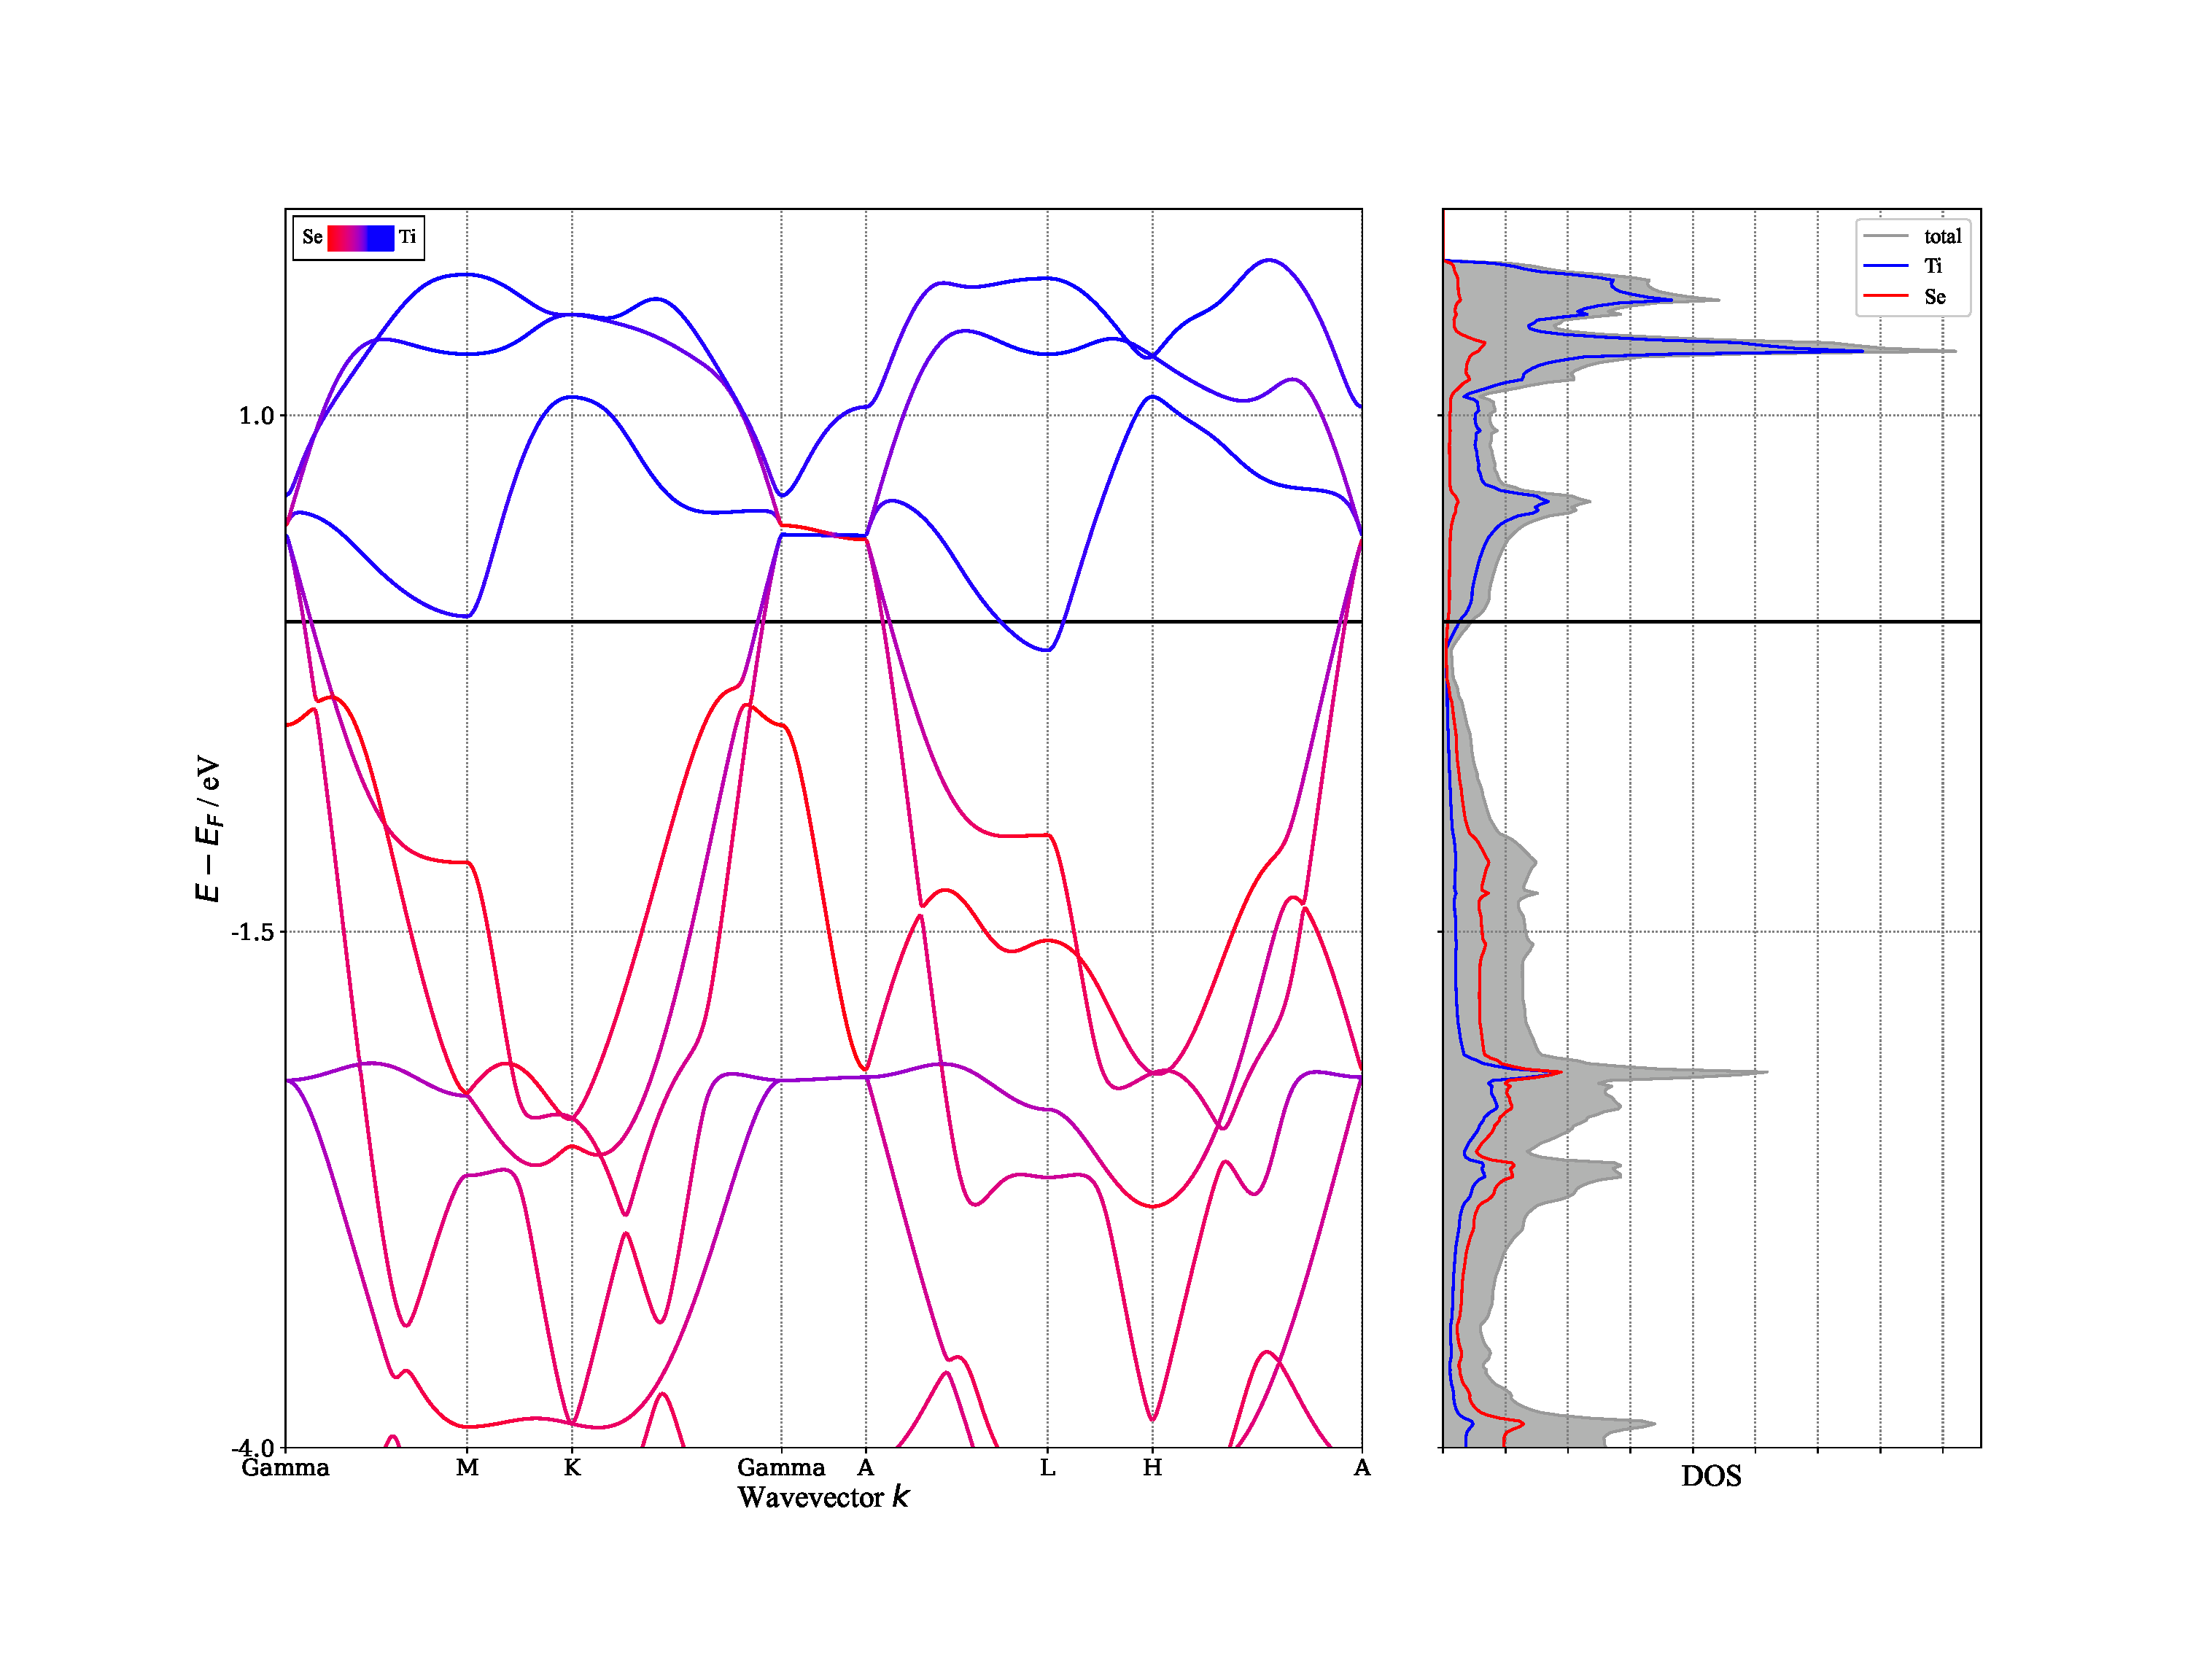
\includegraphics[width=\linewidth]{img/results/TiSe2_GGA_relaxed_BAND+DOS.eps}
    	\caption{
    	TiSe2}
	\end{subfigure}
	\begin{subfigure}[b]{.4\textwidth}
    	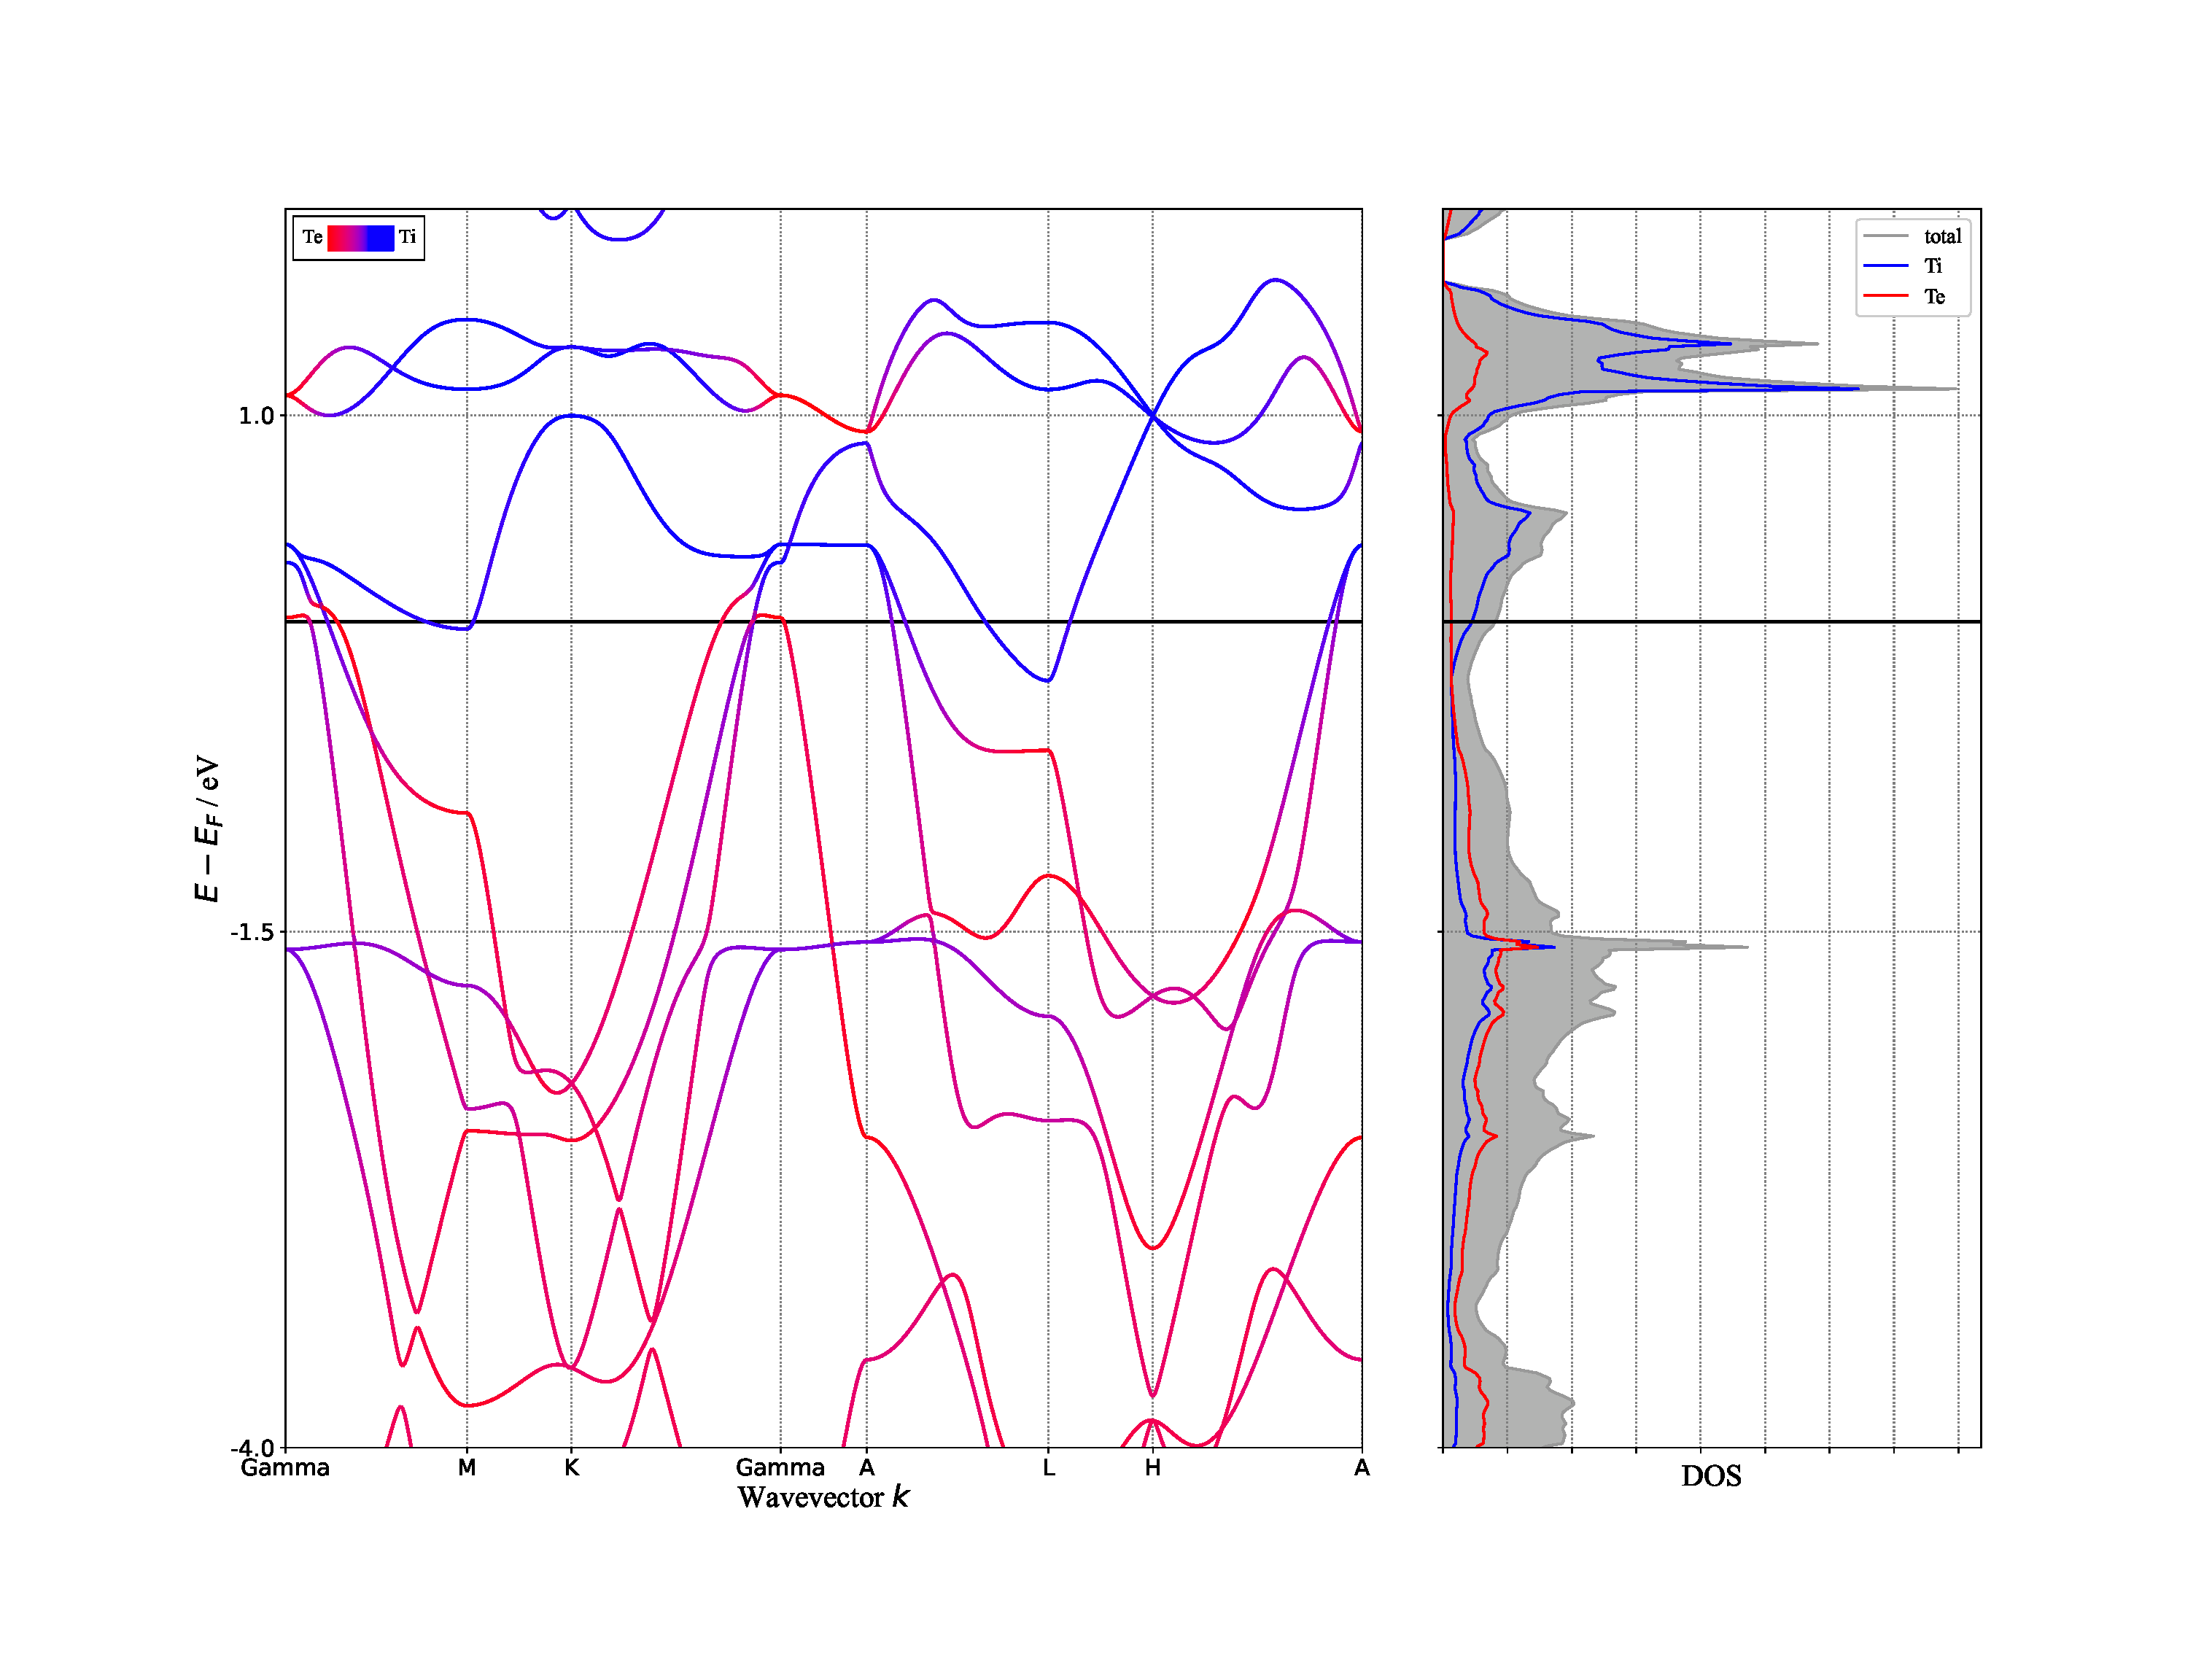
\includegraphics[width=\linewidth]{img/results/TiTe2_GGA_relaxed_BAND+DOS.eps}
    	\caption{
    	TiTe2}
	\end{subfigure}
\caption{Електронна будова TiS$_2$, TiSe$_2$, TiTe$_2$ червоним кольором позначено вклад атомів халькогену (S, Se, Te) синім атомів металу (Ti), розрахована з GGA.}
\label{fig:bandstructireGGA}
\end{figure}

Було визначено що при використані GGA PBE функціоналу, як і очікувалось, відображає зону структуру, що схожа на компенсований метал див. рис. \ref{fig:bandstructireGGA}. На малюнку \ref{fig:fermisurf}, як раз можна побачити, що об'єм електронних карманів приблизно дорівнює об'єму дірок.

\begin{figure}[H]
\centering
	\begin{subfigure}[b]{.4\textwidth}
    	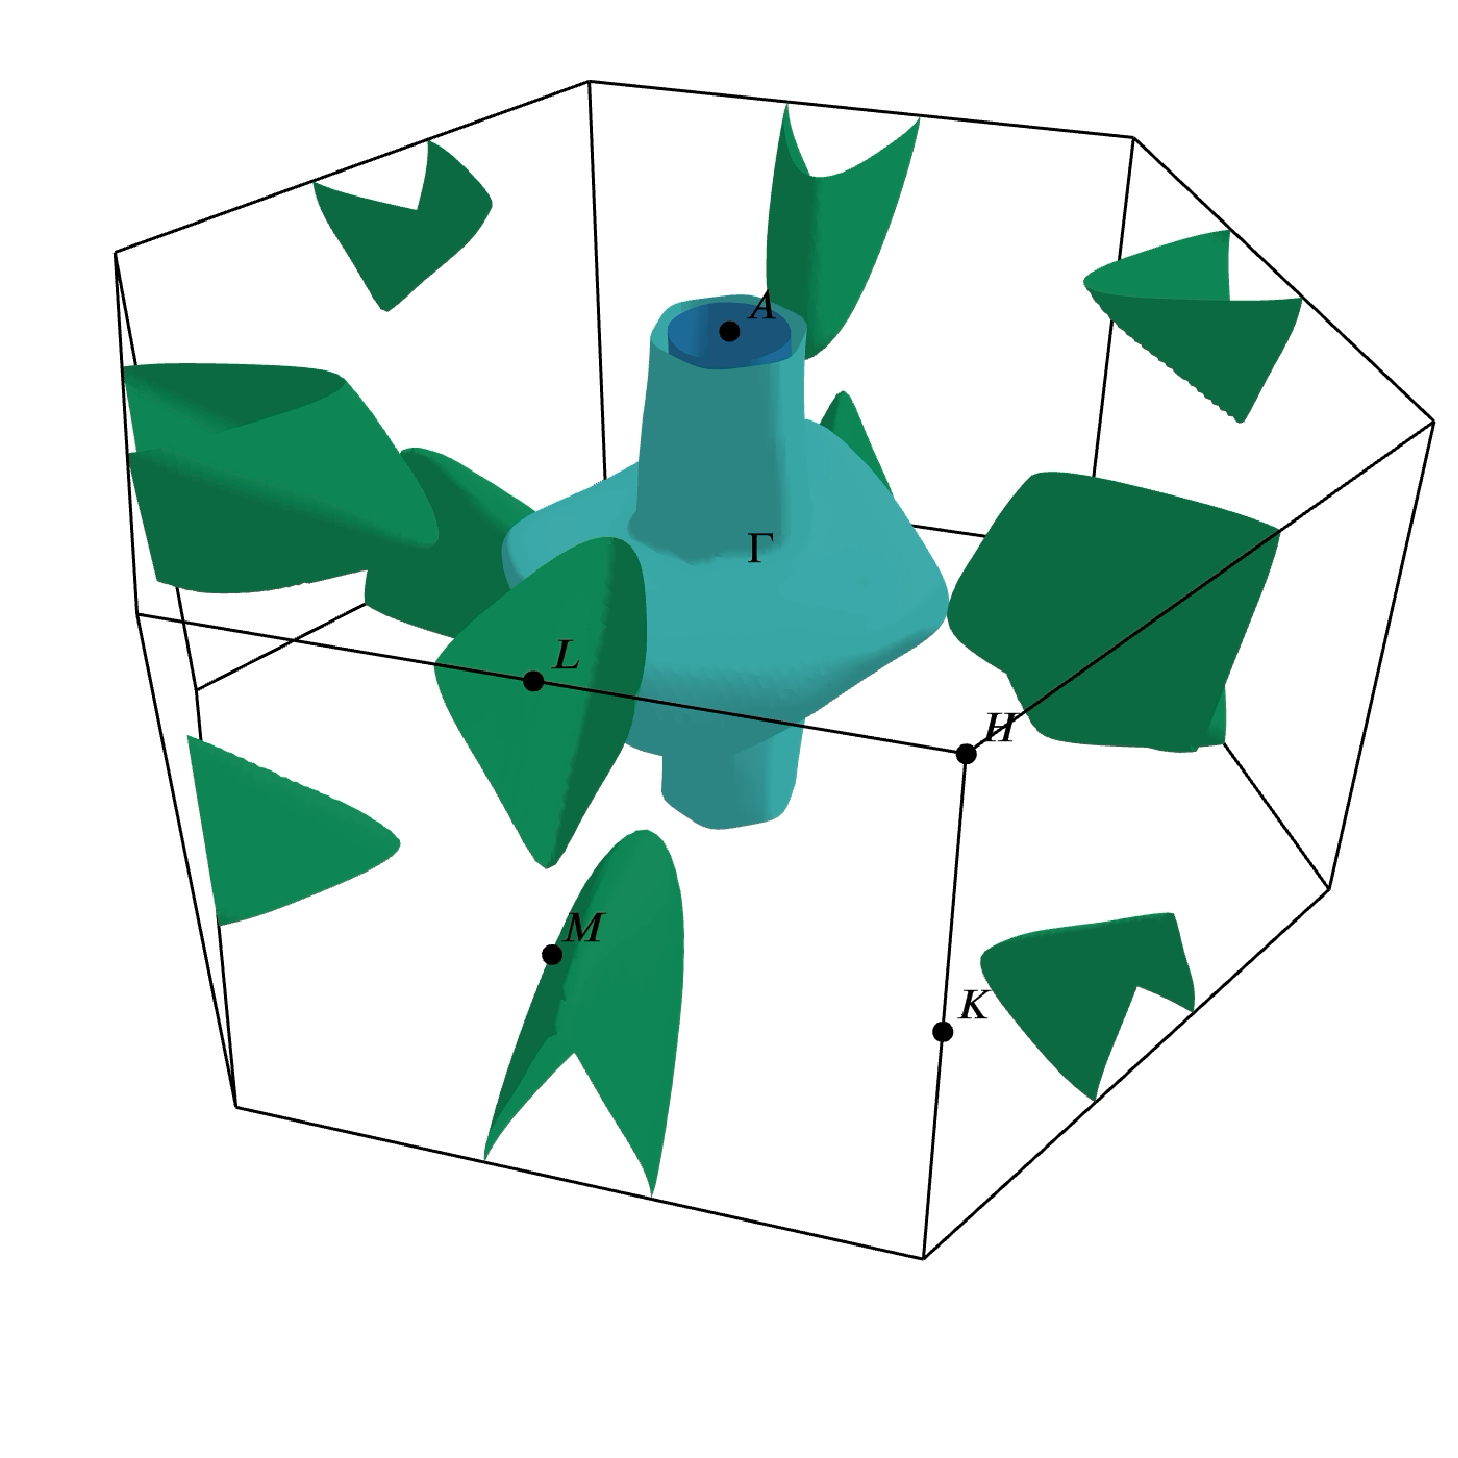
\includegraphics[width=\linewidth]{img/results/fstite2.pdf}
    	\caption{TiTe2}
	\end{subfigure}
	\begin{subfigure}[b]{.4\textwidth}
    	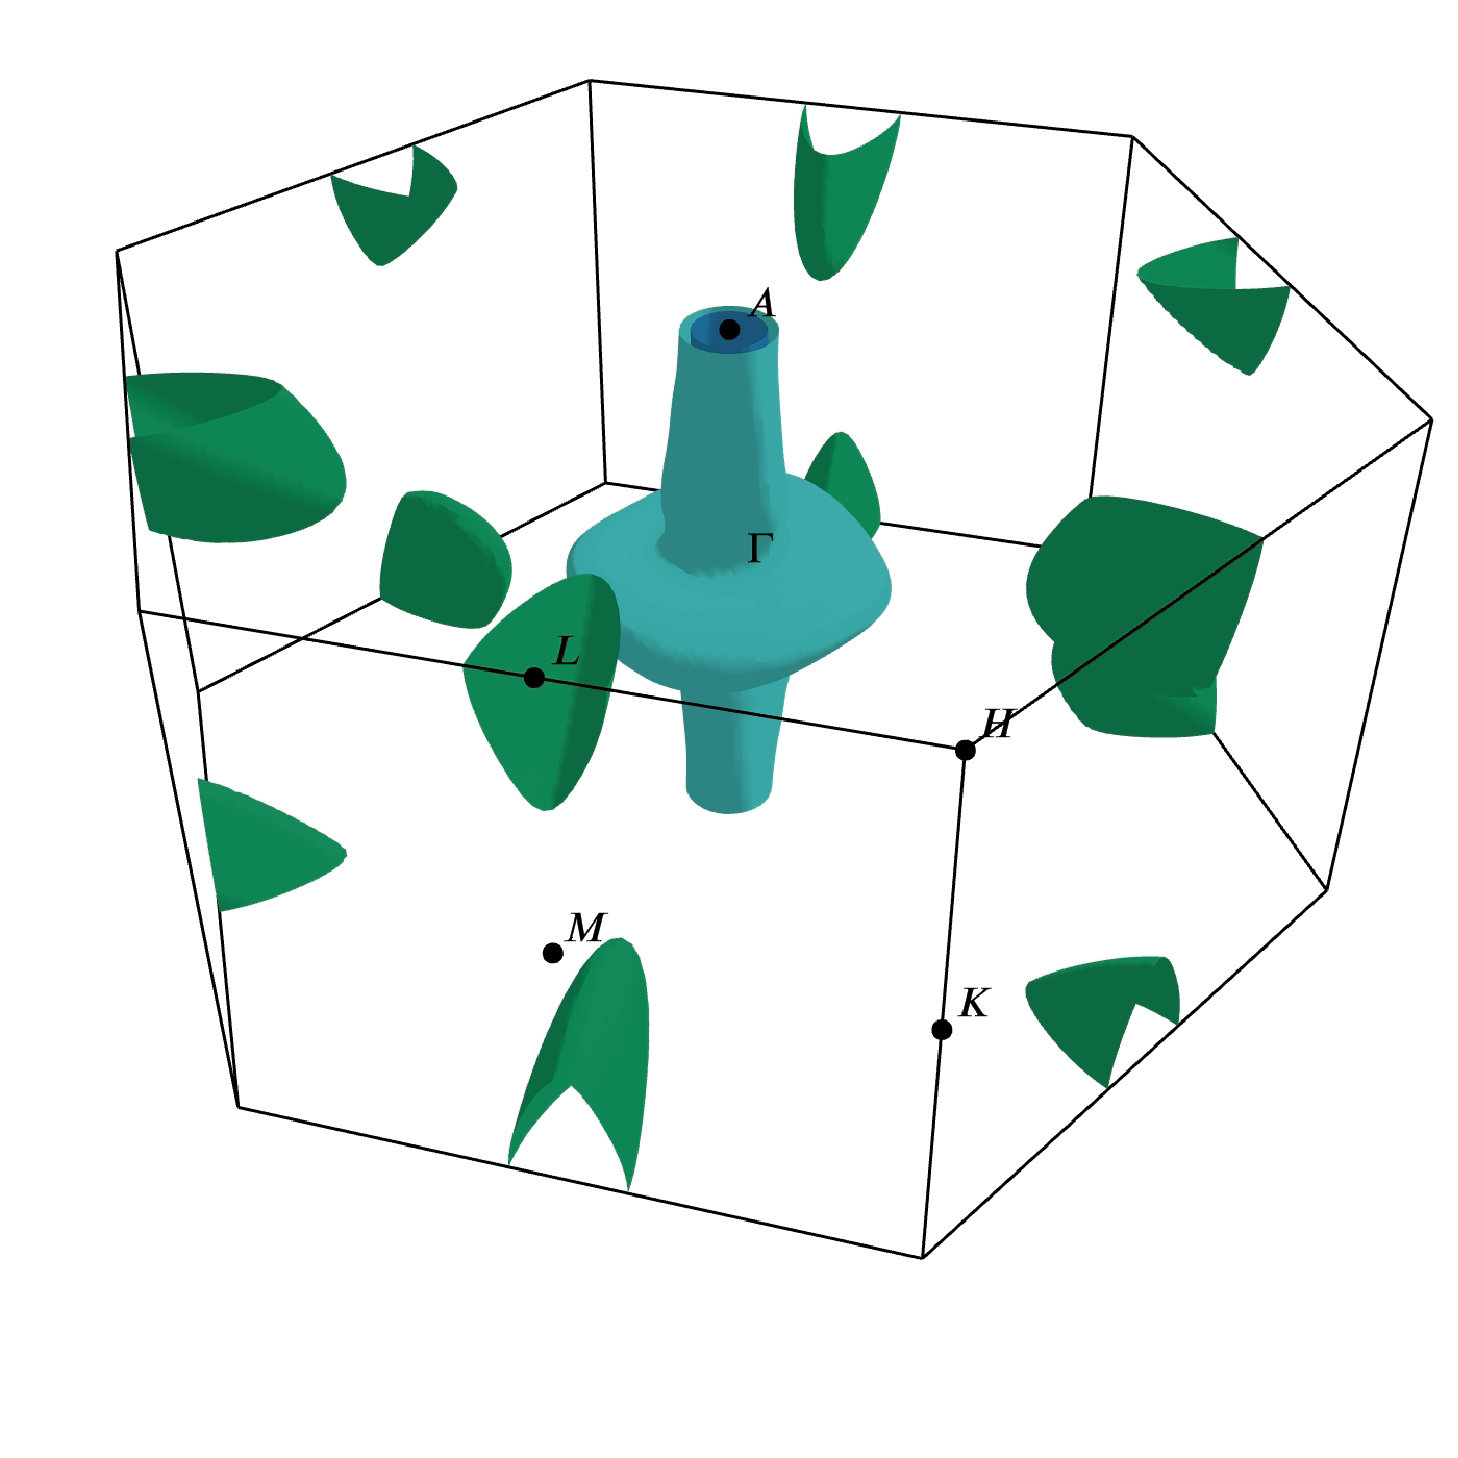
\includegraphics[width=\linewidth]{img/results/fstise2.pdf}
    	\caption{
    	TiSe2}
	\end{subfigure}
	\begin{subfigure}[b]{.9\textwidth}
    	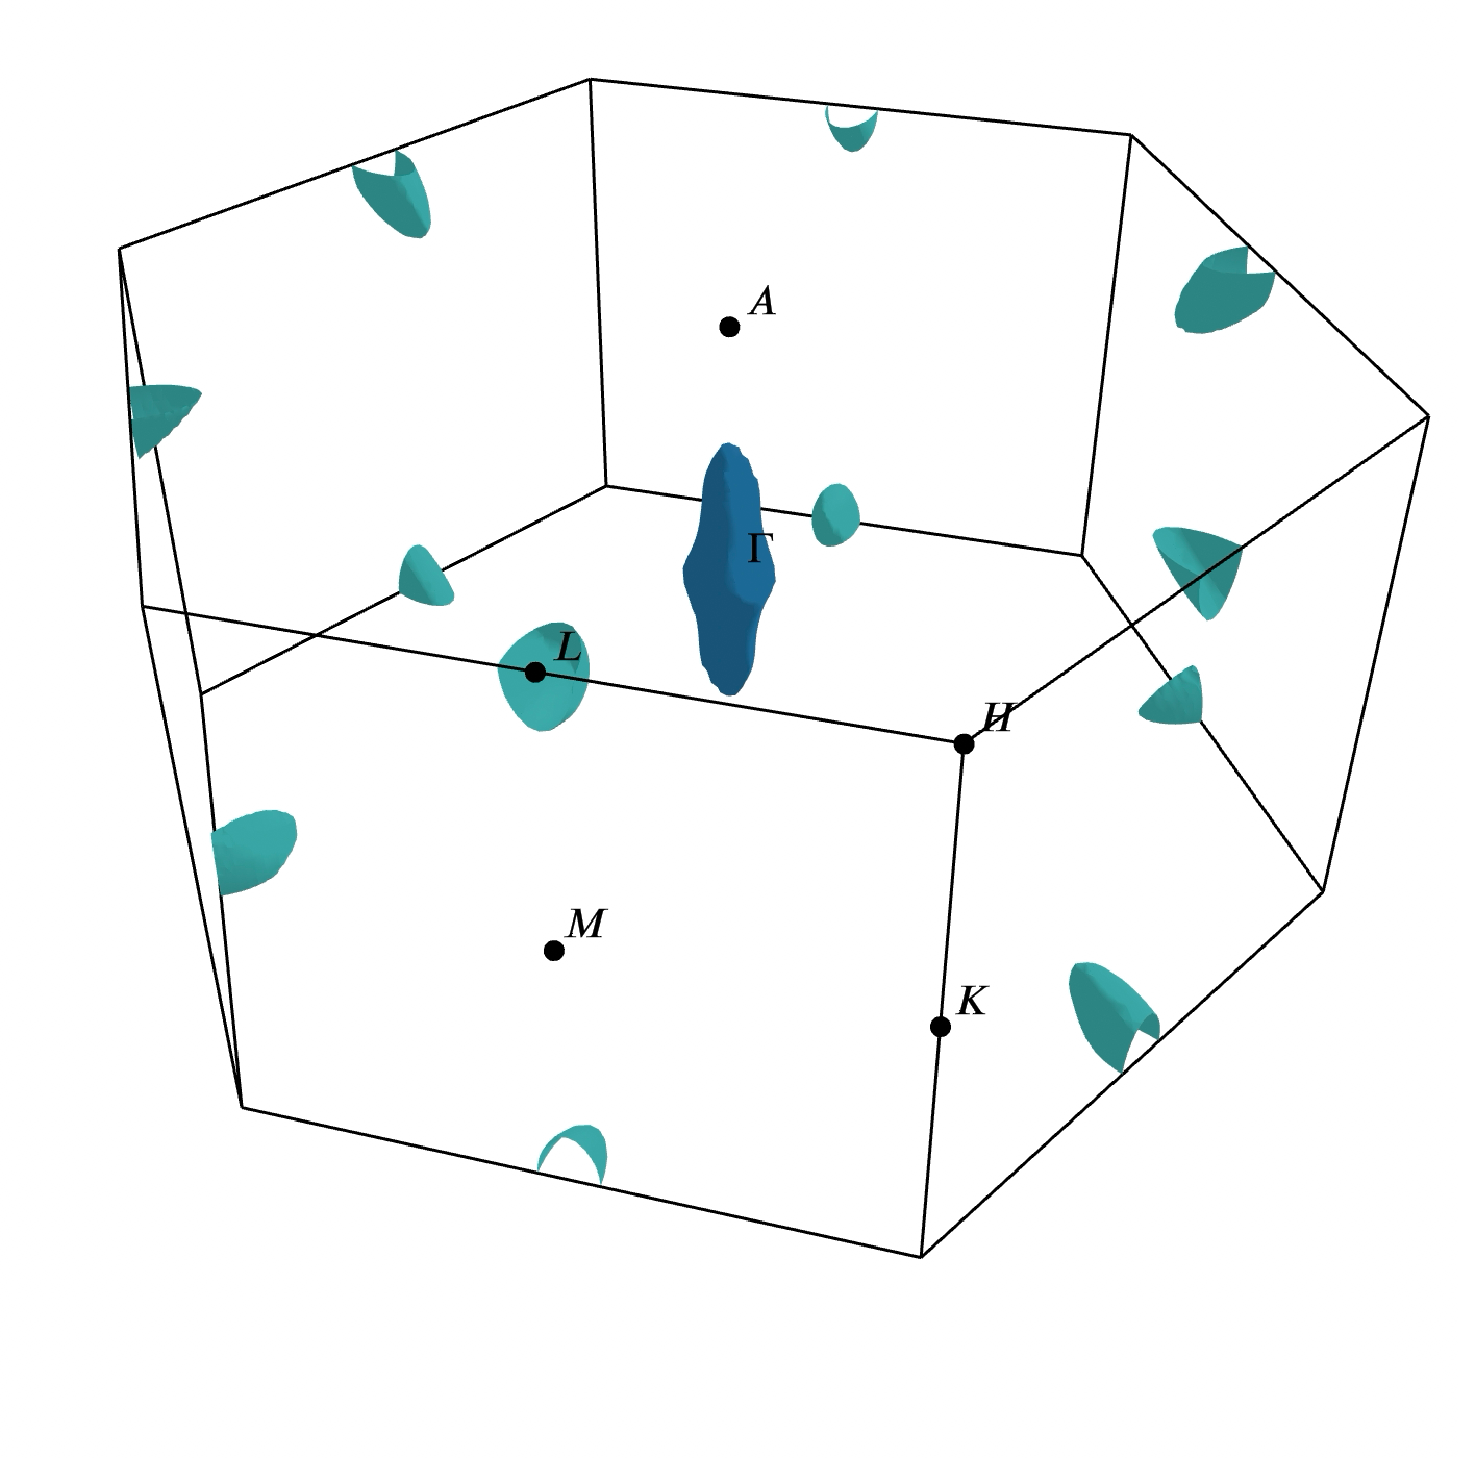
\includegraphics[width=\linewidth]{img/results/fstis2.pdf}
    	\caption{
    	TiS2}
	\end{subfigure}
\caption{Розрахована поверхня фермі TiS$_2$, TiSe$_2$, TiTe$_2$ за допомогою PBE GGA функціоналу.}
\label{fig:fermisurf}
\end{figure}

Після цього було задіяно SCAN функціонал та отримано наступні результати див. мал. \ref{fig:bandstructireSCAN}. Зоні спектри дуже схожі які були розраховані у GGA PBE наближені. Але все ж завдяки тому що SCAN більш точно описує електронну будову ван-дер-Ваальсових матеріалів. То все ж таки перекриття у точці $L$ значно зменшується та становить вже -0.0286 еВ. в $\approx$ 2 менше в порівняні з -0.0633 еВ у GGA PBE. 

\begin{figure}[H]
\centering
	\begin{subfigure}[b]{.9\textwidth}
    	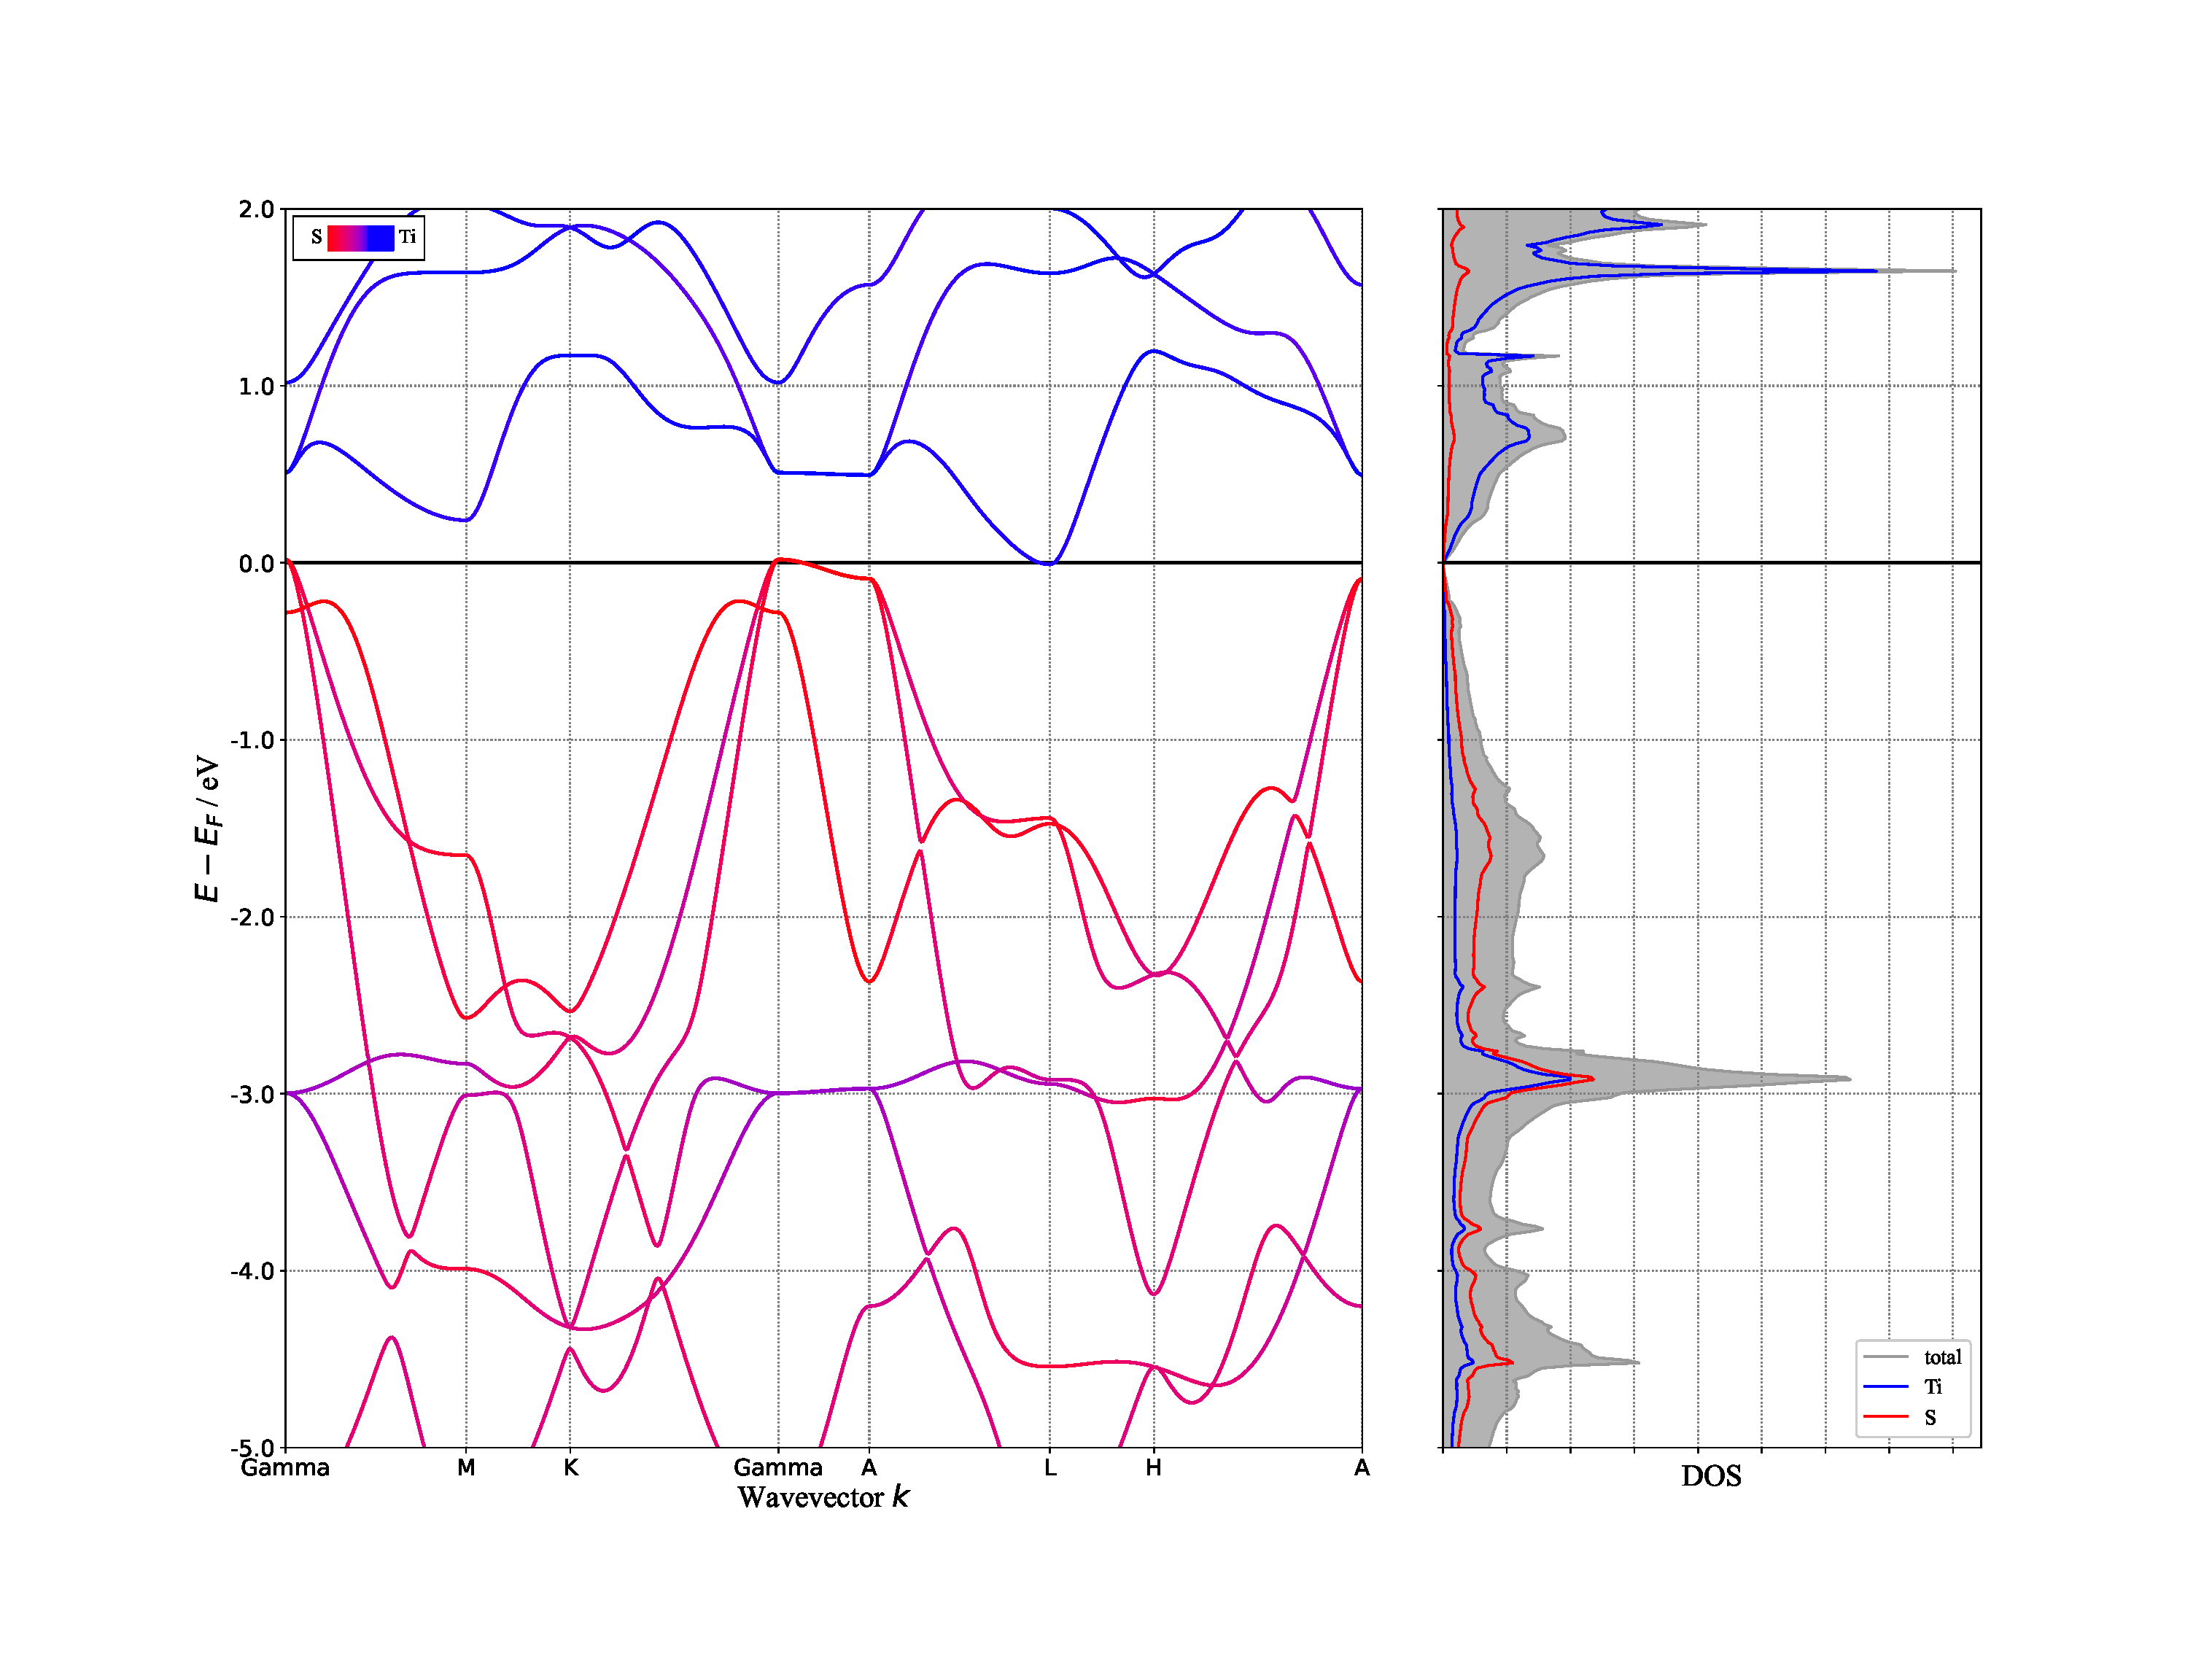
\includegraphics[width=\linewidth]{img/results/TiS2_SCAN_relaxed_BAND+DOS.eps}
    	\caption{TiS2}
	\end{subfigure}
	\begin{subfigure}[b]{.4\textwidth}
    	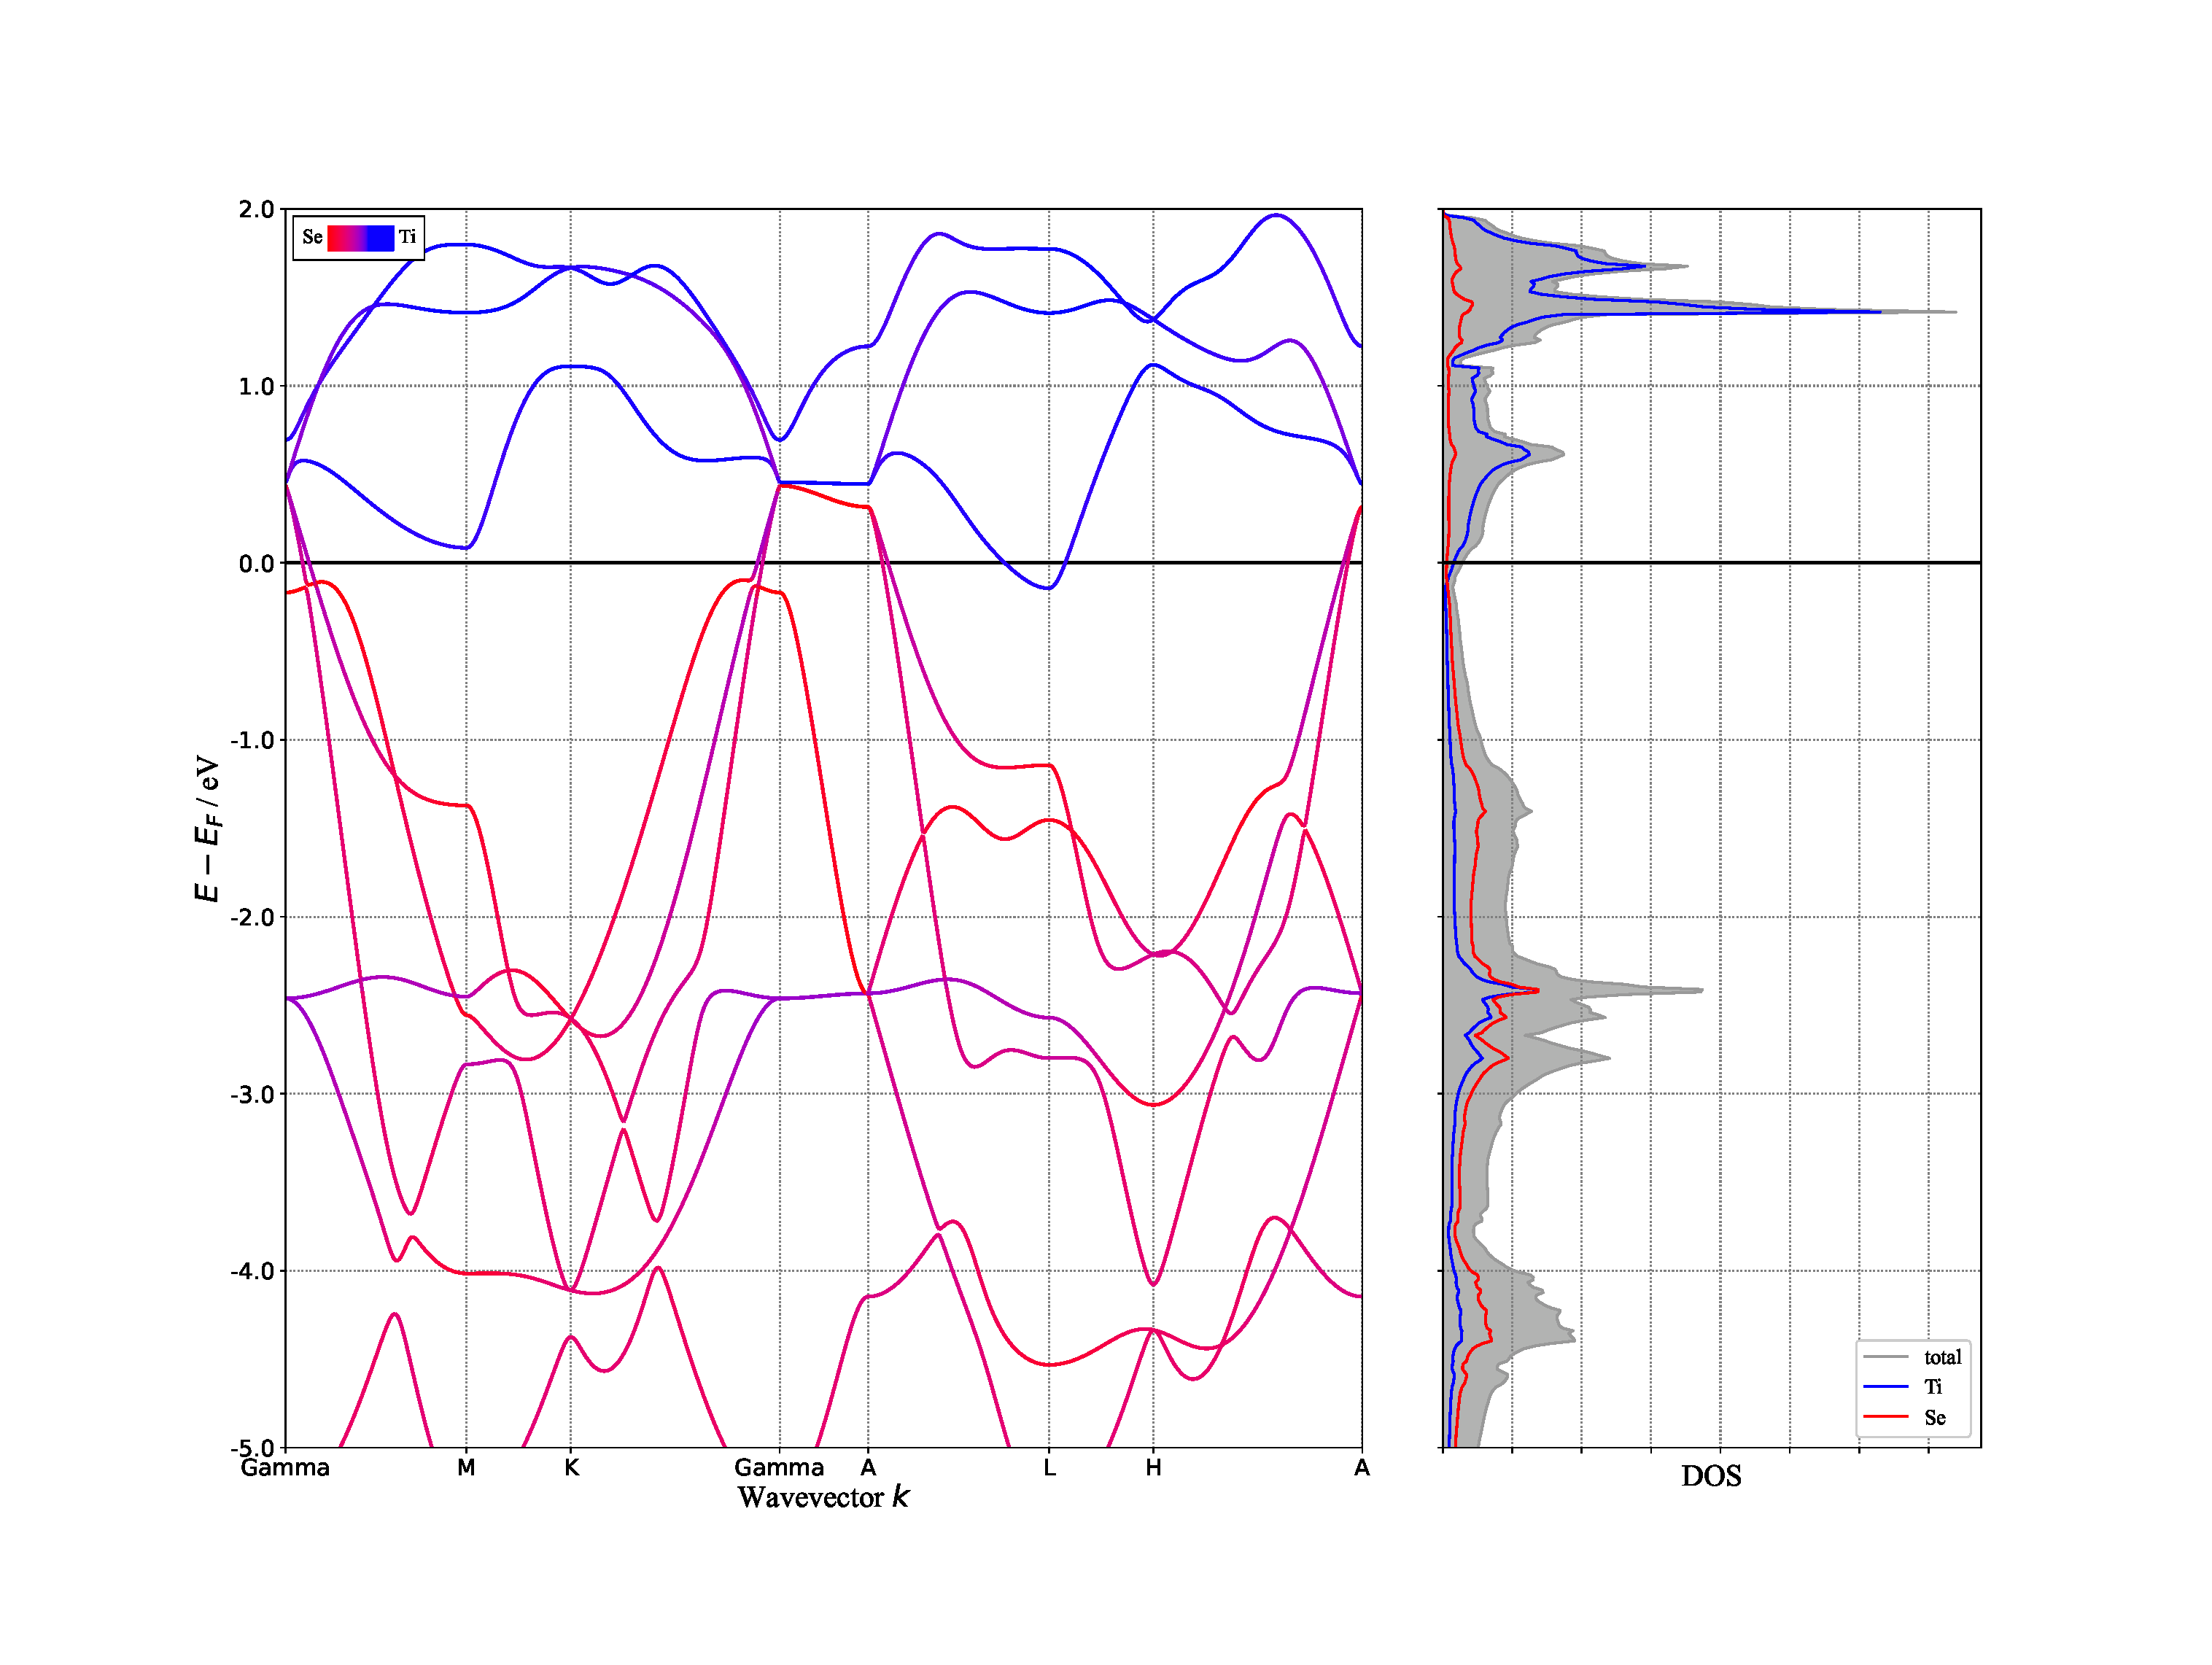
\includegraphics[width=\linewidth]{img/results/TiSe2_SCAN_relaxed_BAND+DOS}
    	\caption{
    	TiSe2}
	\end{subfigure}
	\begin{subfigure}[b]{.4\textwidth}
    	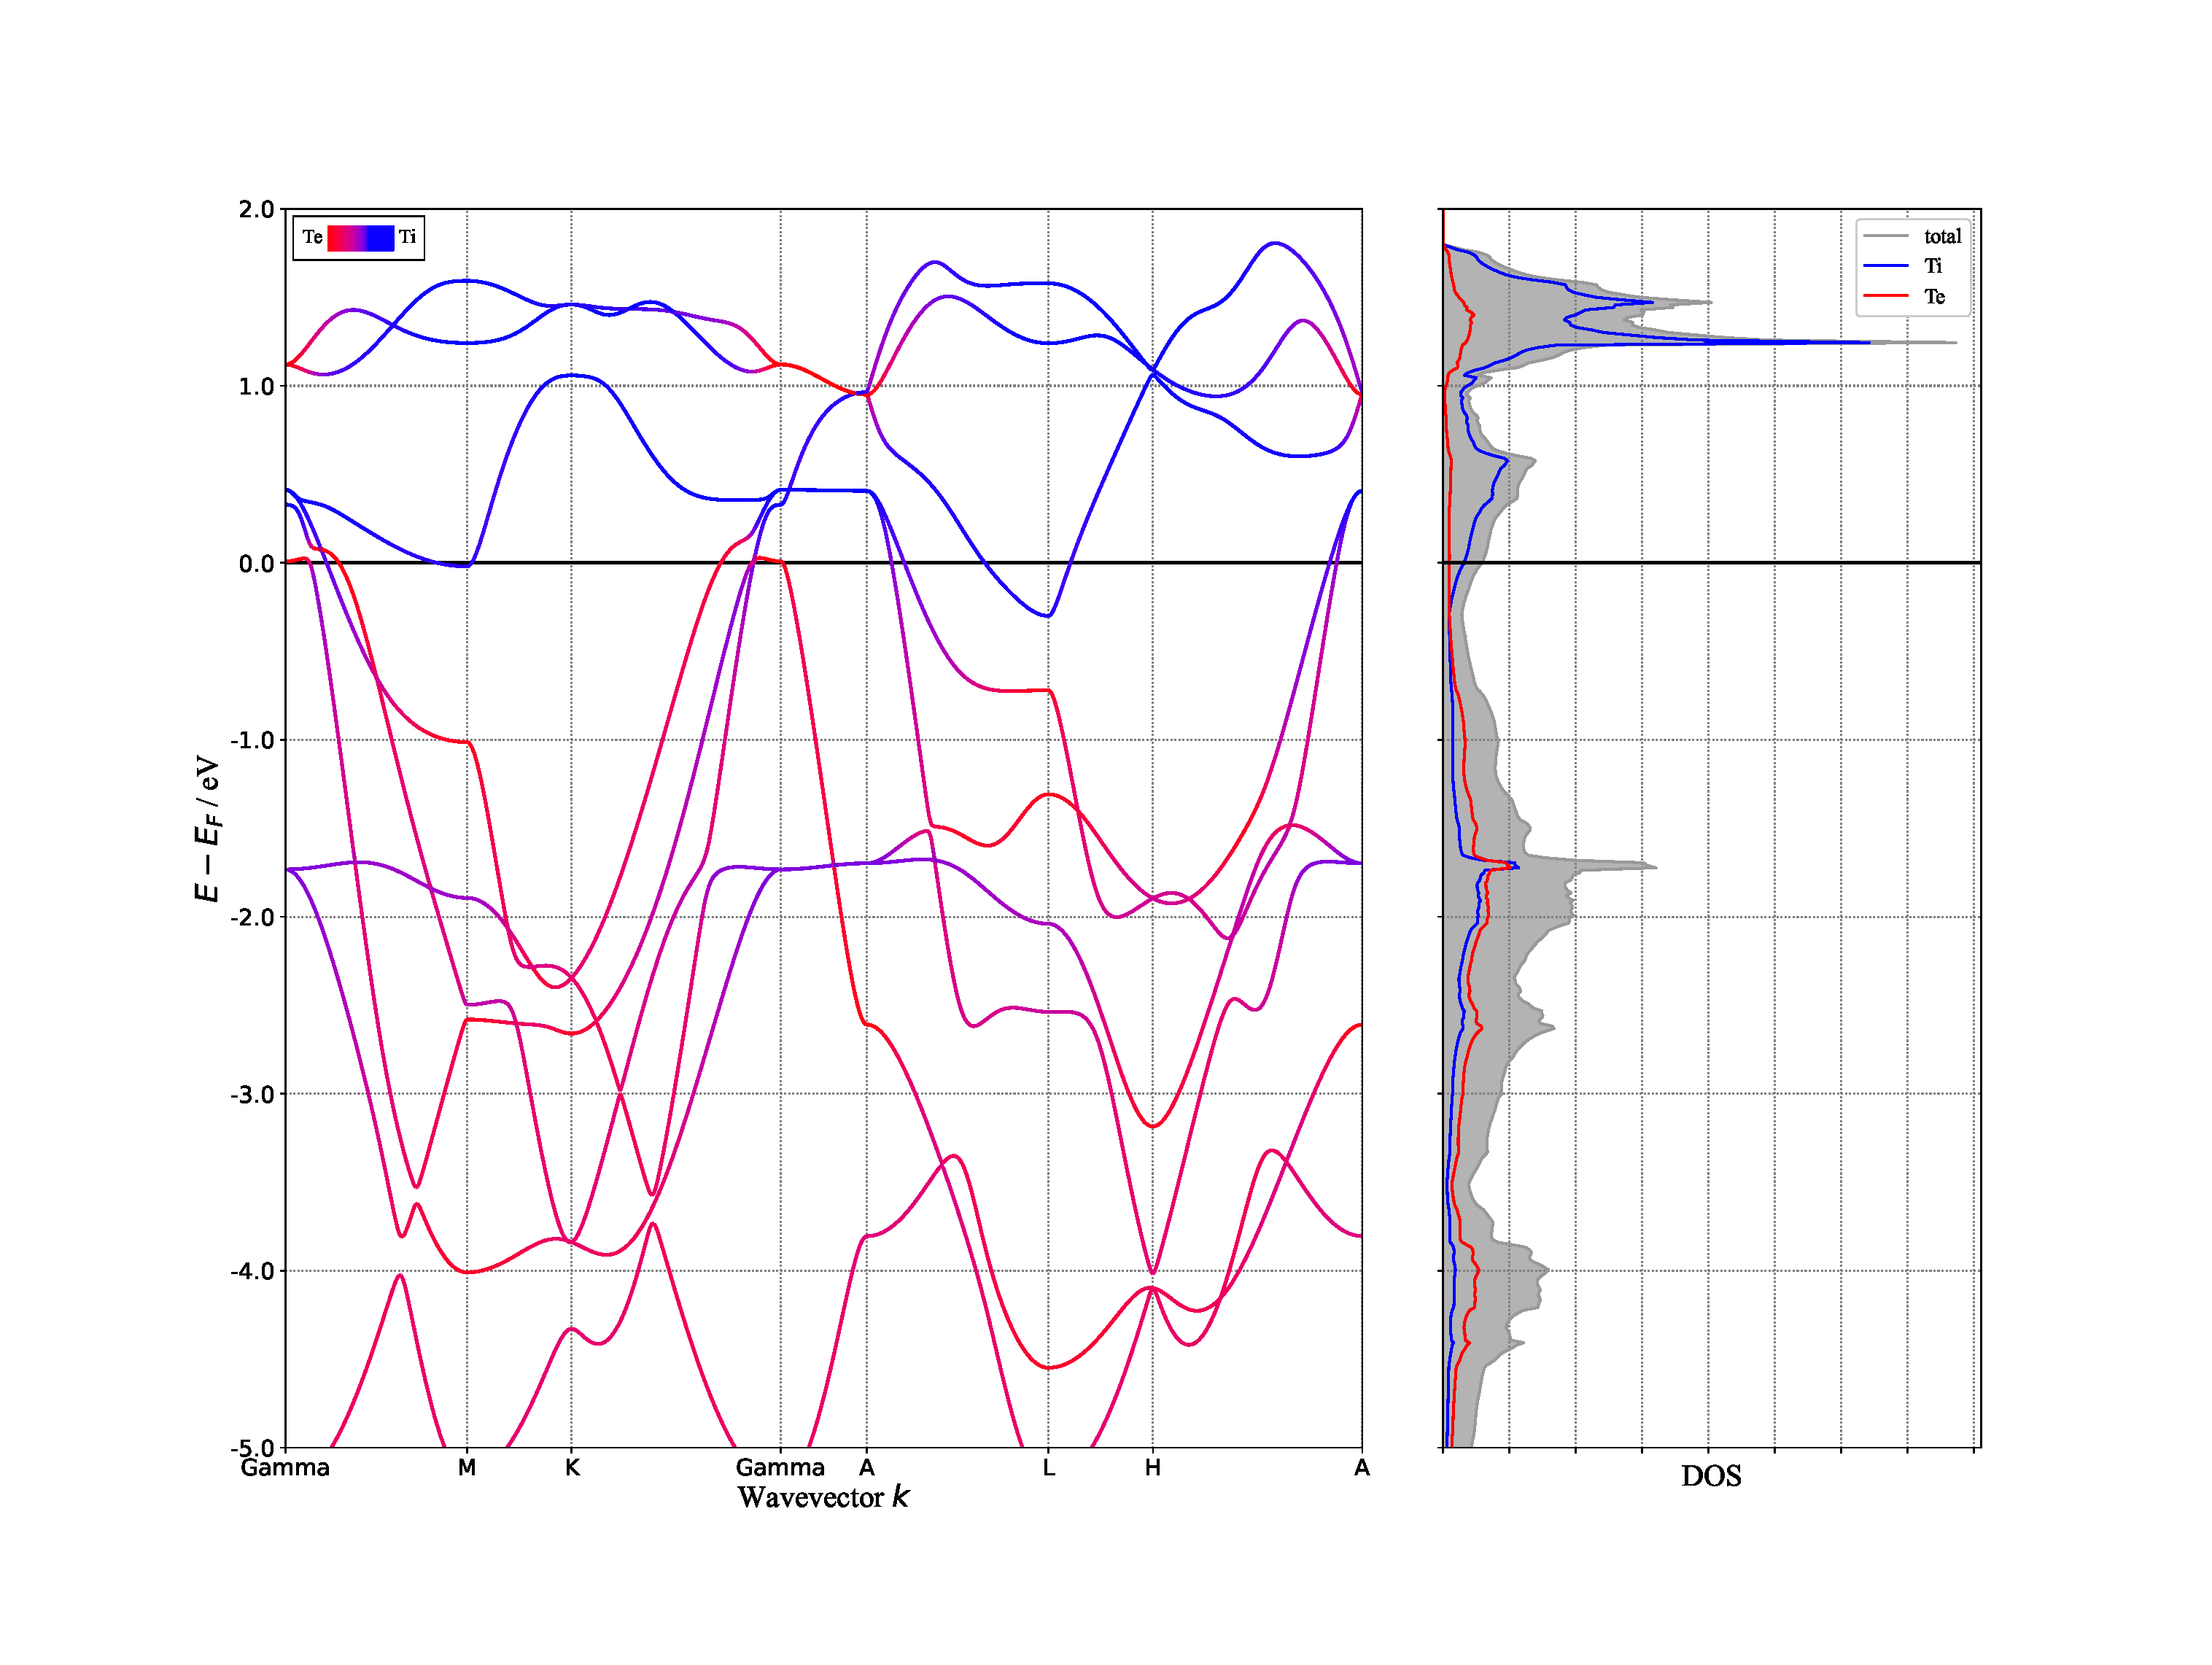
\includegraphics[width=\linewidth]{img/results/TiTe2_SCAN_relaxed_BAND+DOS}
    	\caption{
    	TiTe2}
	\end{subfigure}
\caption{Електронна будова TiS$_2$, TiSe$_2$, TiTe$_2$ червоним кольором позначено вклад атомів халькогену (S, Se, Te) синім атомів металу (Ti), розрахована з SCAN.}
\label{fig:bandstructireSCAN}
\end{figure}

Для того щоб показати наскільки матеріал сильно корельований ми за референс брали саме TiS$_2$ сполуку, закріпляли координати атомів елементарної комірки та варіювали U до 3.0 еВ див. рис. \ref{fig:variationU_GGA}. 

\begin{figure}
	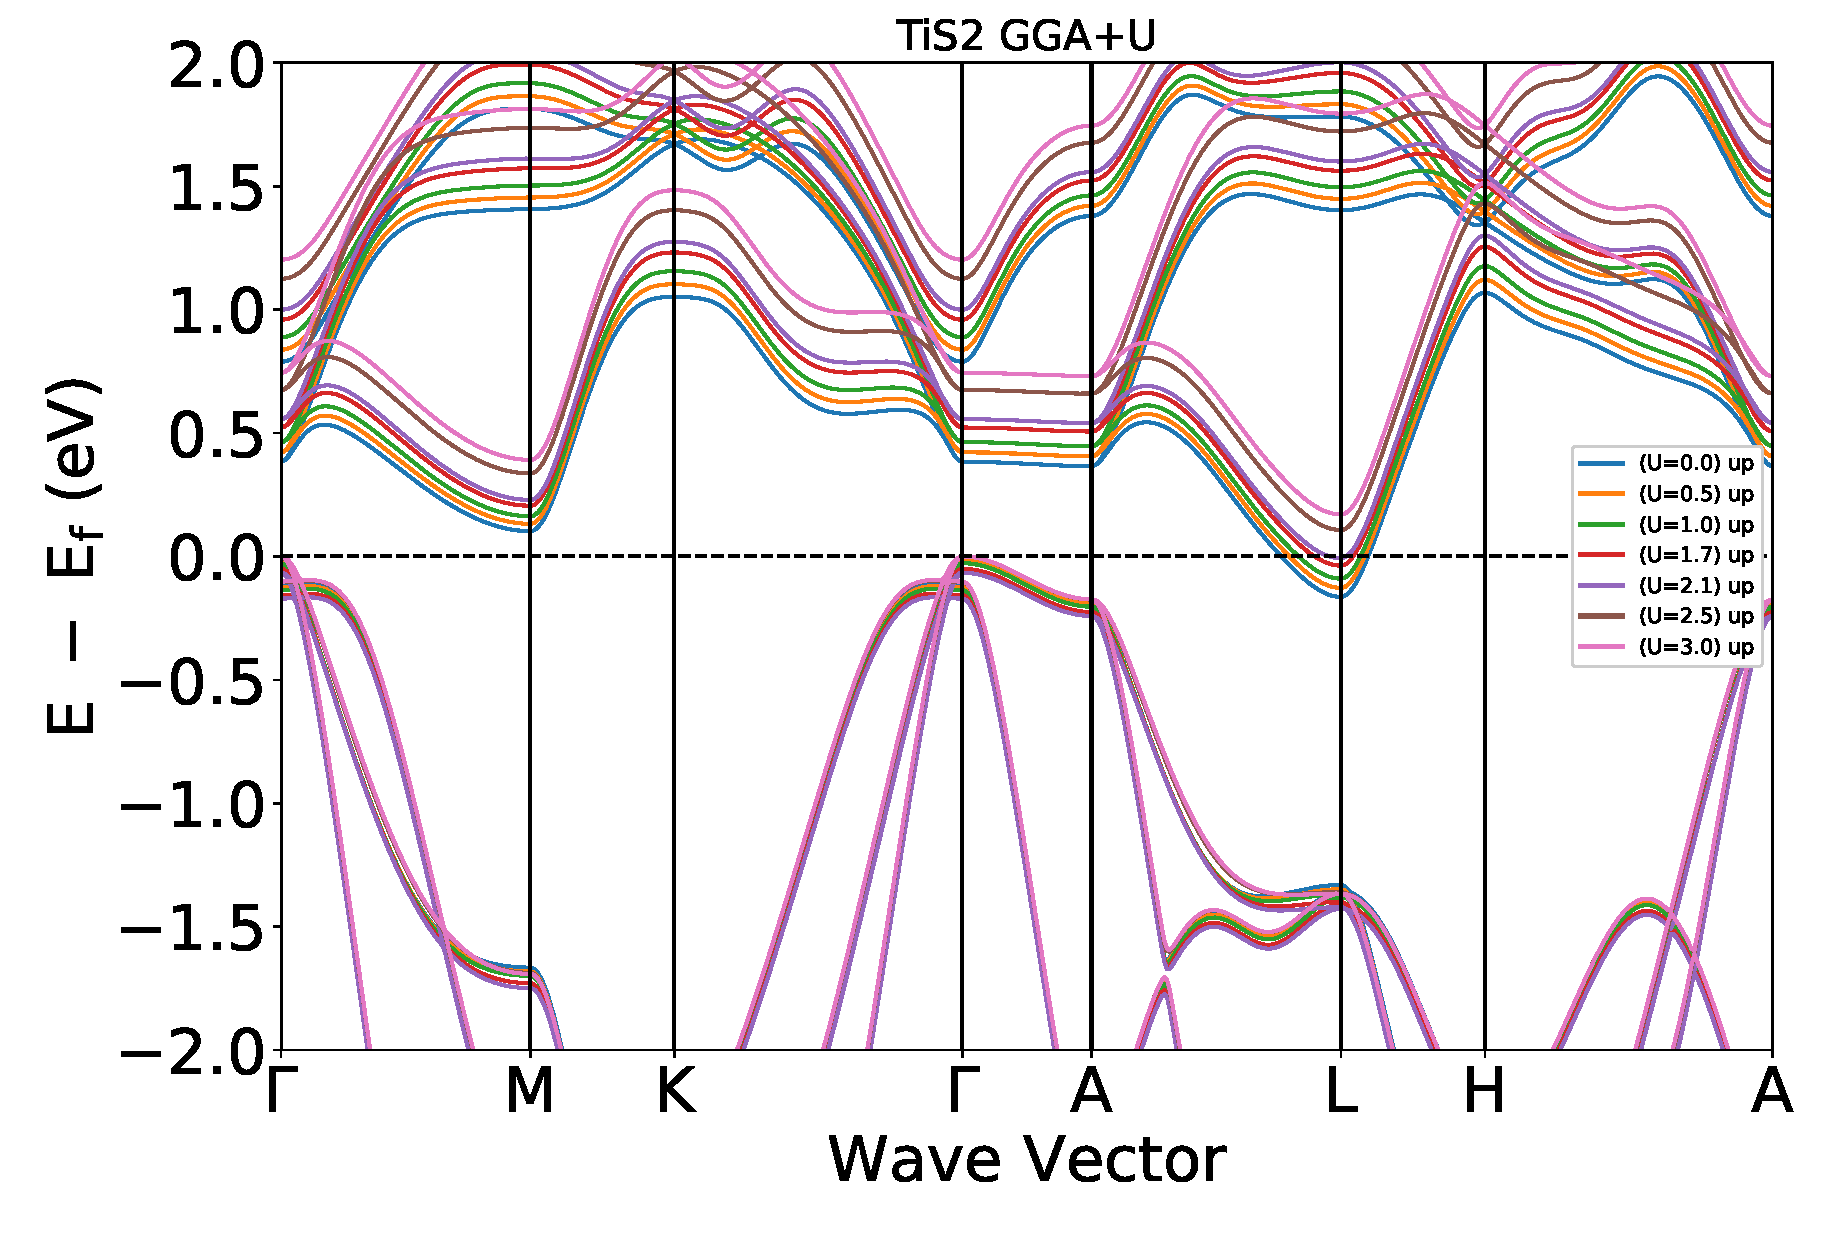
\includegraphics[scale=0.6]{results/TiS2_GGA+U--variation.eps}
	\caption{Зонна структура при варіації U від 0 до 3.0 eV, для TiS$_2$.}
	\label{fig:variationU_GGA}
\end{figure}

Як зазначалось у попередніх розділах, для опису сильнокорельованих систем ми маємо використовувати DFT+U. При прикладених U зонна щілина відкривається таб. \ref{tab:VariationU} на 0.0129 еВ при $U=1.7$ та 0.0587 еВ при $U=2.1$, але цього недостатньо, щоб чітко стверджувати, ща ми маємо напівпровідникову поведінку матеріалу. 

\begin{table}[H]\centering
\scriptsize
\begin{tabular}{lrr}\toprule
\multicolumn{2}{c}{\textbf{Варіація U }} \\\midrule
\multirow{2}{*}{\textbf{U}} &\multirow{2}{*}{\textbf{Band Gap}} \\
& \\
0.0 & -0.1609 \\
0.5 &-0.1134 \\
1.0 &-0.0631 \\
1.7 &0.0129 \\
2.1 &0.0587 \\
2.5 &0.1067 \\
3.0 &0.1699 \\
\bottomrule
\end{tabular}
\caption{Перетин $p$ орбіталей у точці $L$ з варіацією U для TiS$_2$.}\label{tab:VariationU}
\end{table}

Також з даного малюнку можна сказати те, що при збільшені $U=2.5, 3.0$ еВ ми бачимо, як щілина збільшується між $\Gamma$ та $L$ точками. Та при нескінченному збільшені $U$ ми можемо отримати майже будь-яку ширину забороненої зони, але в цей момент постає питання, наскільки адекватна структура комірки буде описуватись? При збільшені $U$ ми будемо мати збільшення напруження в решітці і фактично ми вже будемо розраховувати "інший" зразок. До таких самих висновків приходять для схожого матеріалу TiO$_2$ \cite{doi:10.1063/1.3617244}. Тому ми обираємо $U=2.1$ eV для наступних розрахунків.

\begin{figure}[H]
	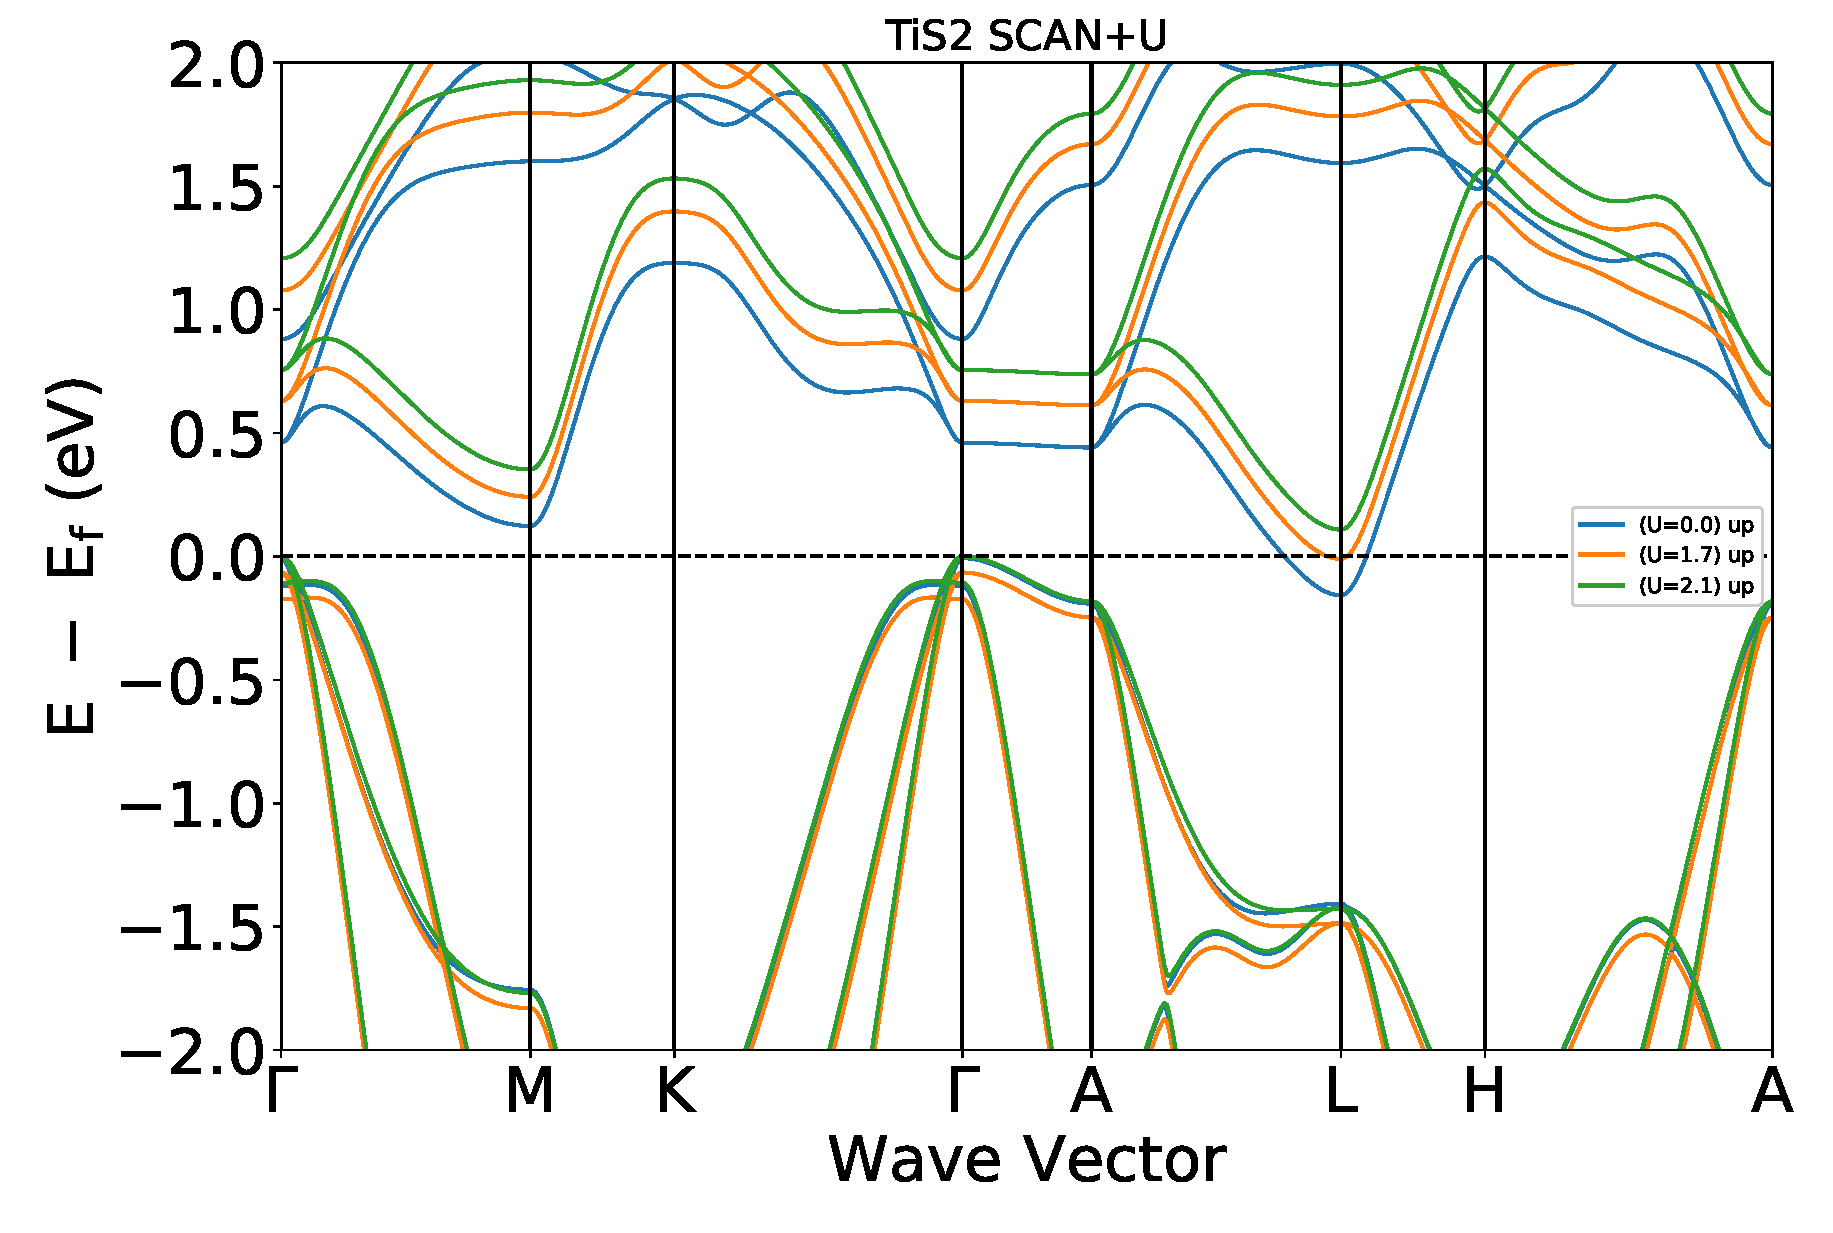
\includegraphics[scale=0.6]{results/TiS2_SCAN+U-variation.eps}
	\caption{Електронна будова TiS$_2$ SCAN + U (U = 0, 1.7, 2.1).}\label{fig:SCAN+U_1.7_2.1}
\end{figure}

Варіюючи U зі значеннями 1.7 еВ, 2.1 еВ рис. \ref{fig:SCAN+U_1.7_2.1} ми отримуємо щілину при таких самих значеннях, що і при GGA+U, але розмір цієї щілини на відміно від GGA PBE, вже узгоджується з розрахунками іншими методами та експериментами. При використанні функціоналу SCAN+U (U = 2.1 eV) ми бачимо, як відкривається зонна щілина порядку $\approx$ 0.1 eV у сполуці TiS$_2$ див. рис. \ref{fig:SCAN+U_tis2}, але цього не відбувається у TiSe$_2$, TiTe$_2$ див. рис. \ref{fig:SCAN+U_tise2}, \ref{fig:SCAN+U_tite2} і це узгоджується з експериментальними даними.

\begin{figure}[H]
	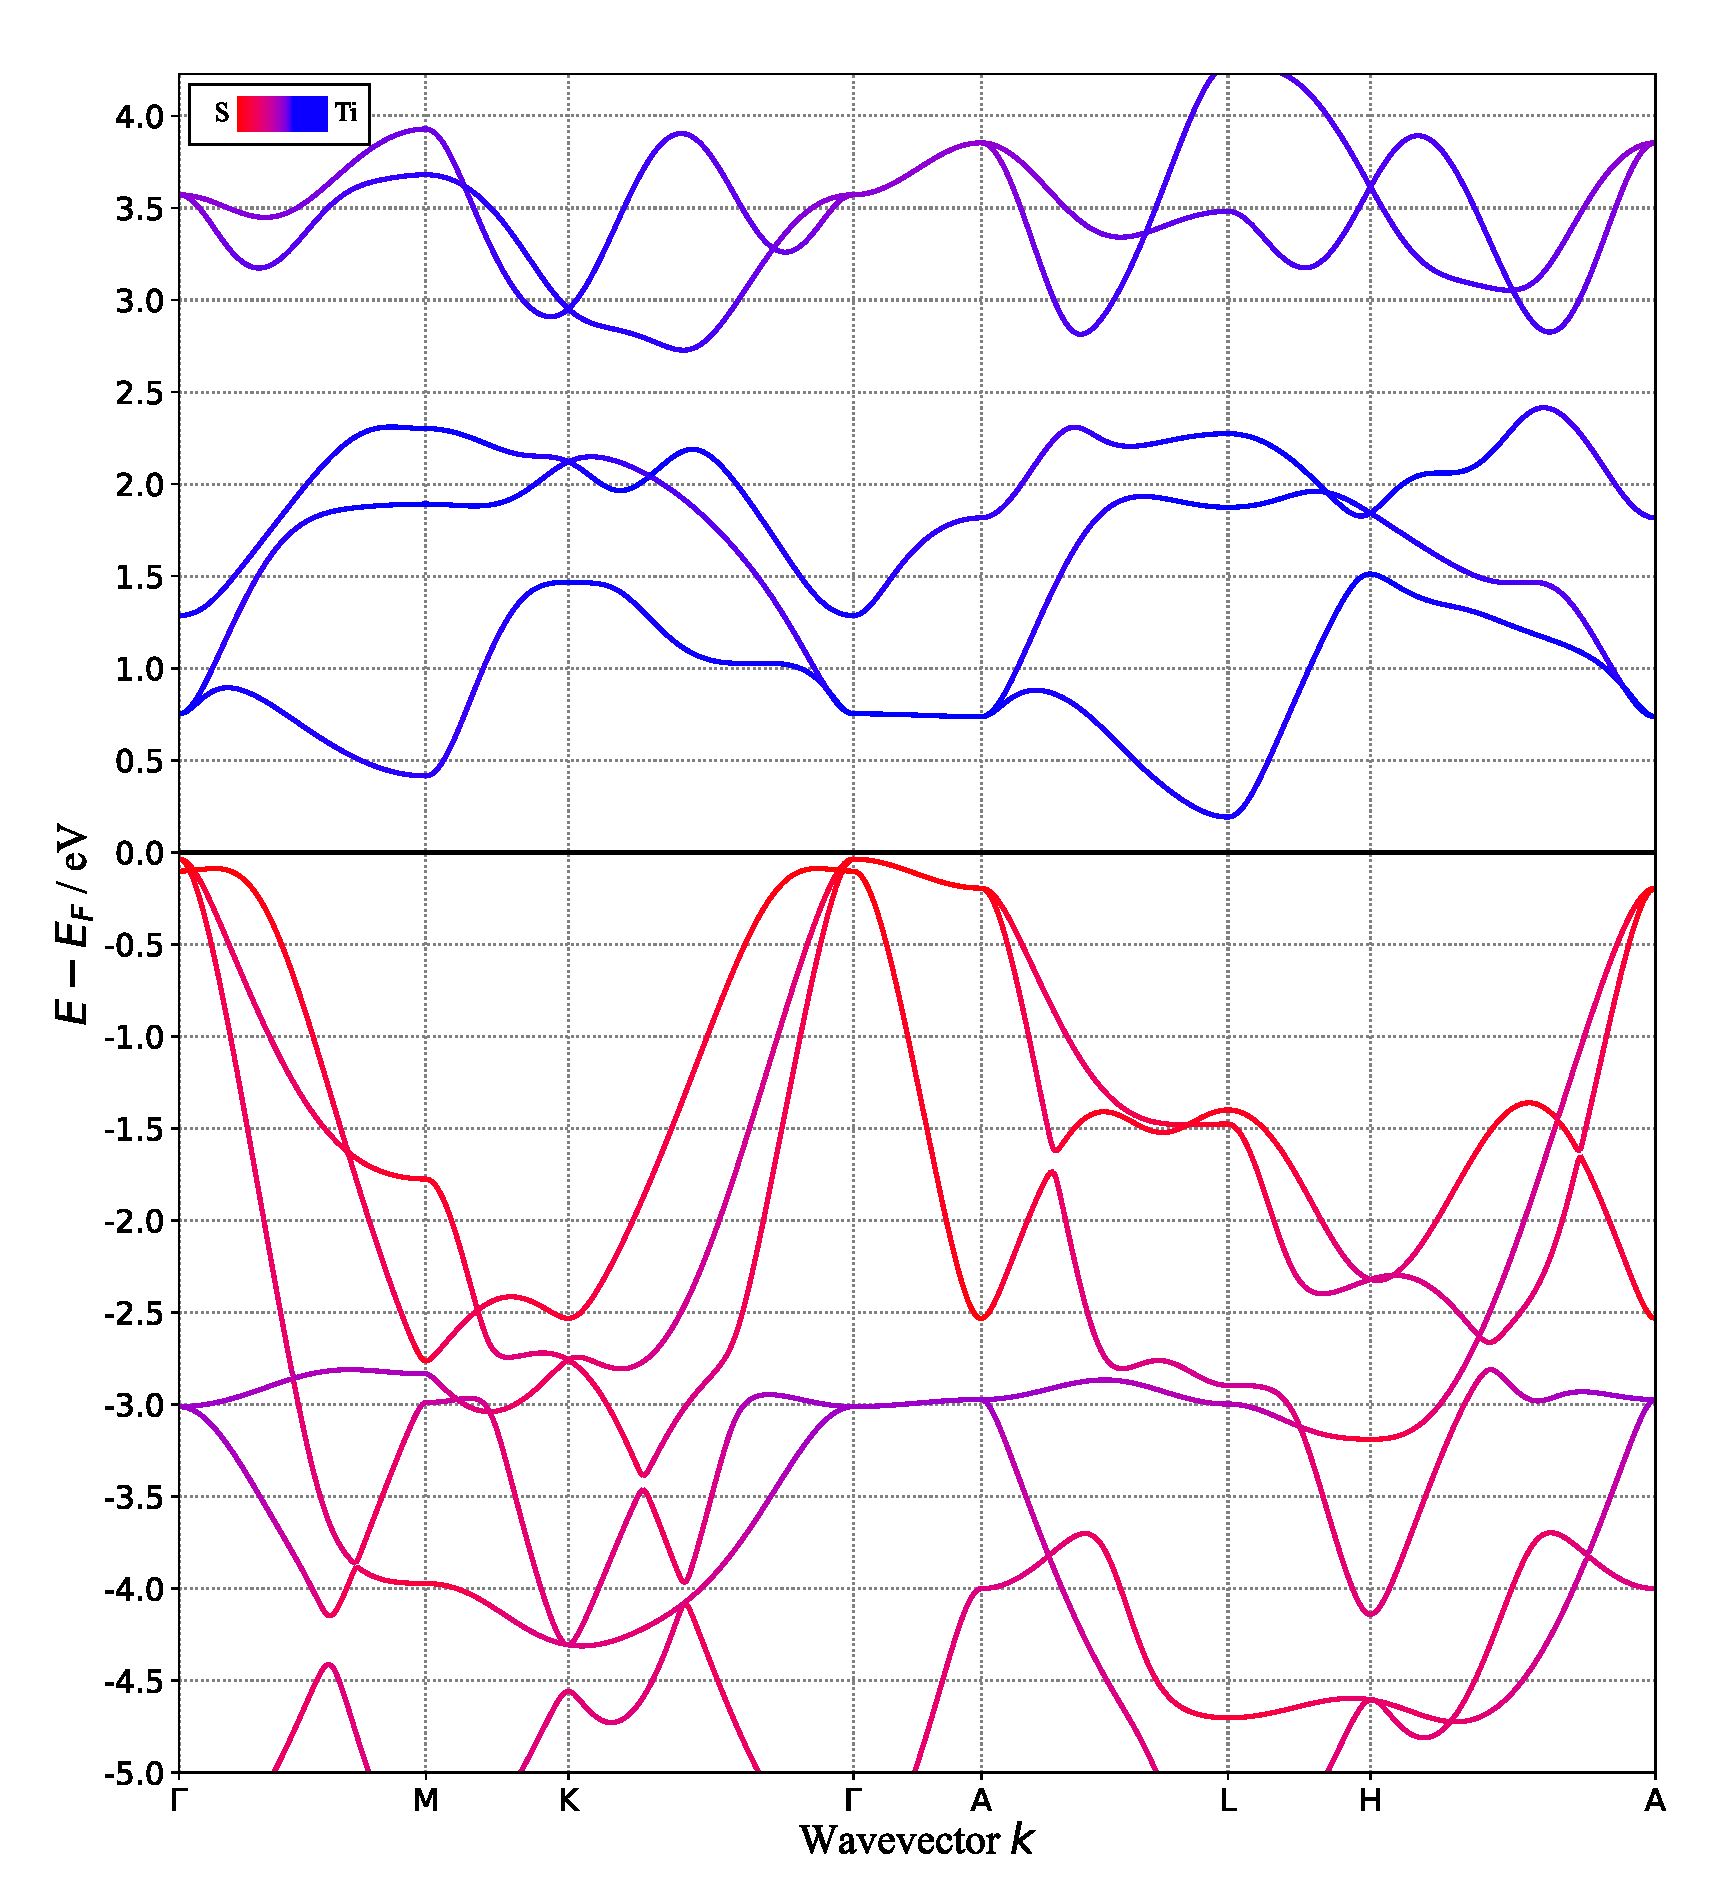
\includegraphics[scale=0.6]{results/SCAN-rVV10+U}
	\caption{Електронна будова TiS$_2$ з використанням поправок rVV10.}\label{fig:rVV10+U}
\end{figure}

Після цього було використано для структурної релаксації вандервальсовські поправки \cite{Peng_2016}, які більш краще описують геометрію решітки та отримати вже наближене до експериментального значення розмір щілини $\approx$ 0.22 eV. див. рис. \ref{fig:rVV10+U}.

\begin{figure}
	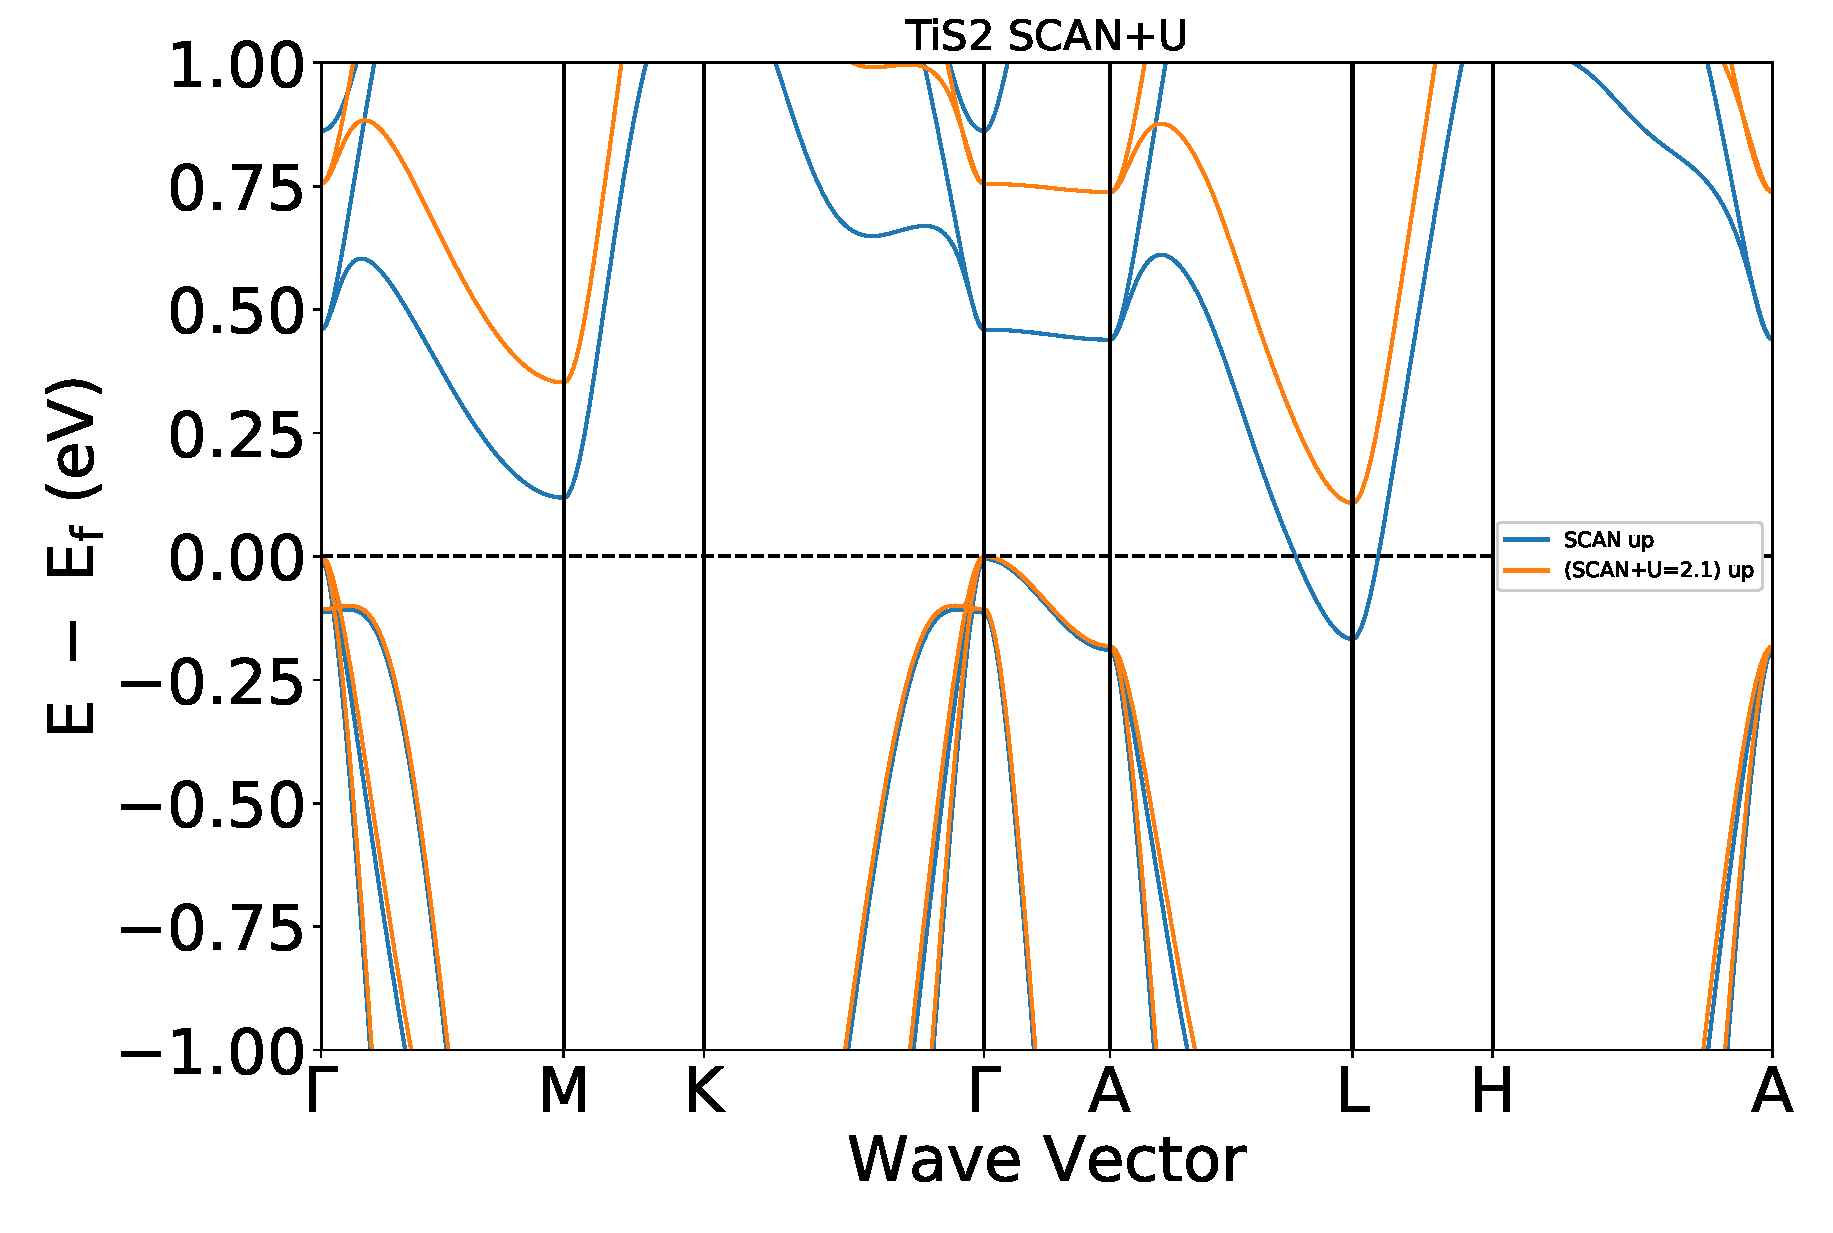
\includegraphics[scale=0.6]{results/TiS2_SCAN_vs._SCAN+U.eps}
	\caption{Електрона будова TiS$_2$ SCAN + U (U = 2.1).}\label{fig:SCAN+U_tis2}
\end{figure}

\begin{figure}
	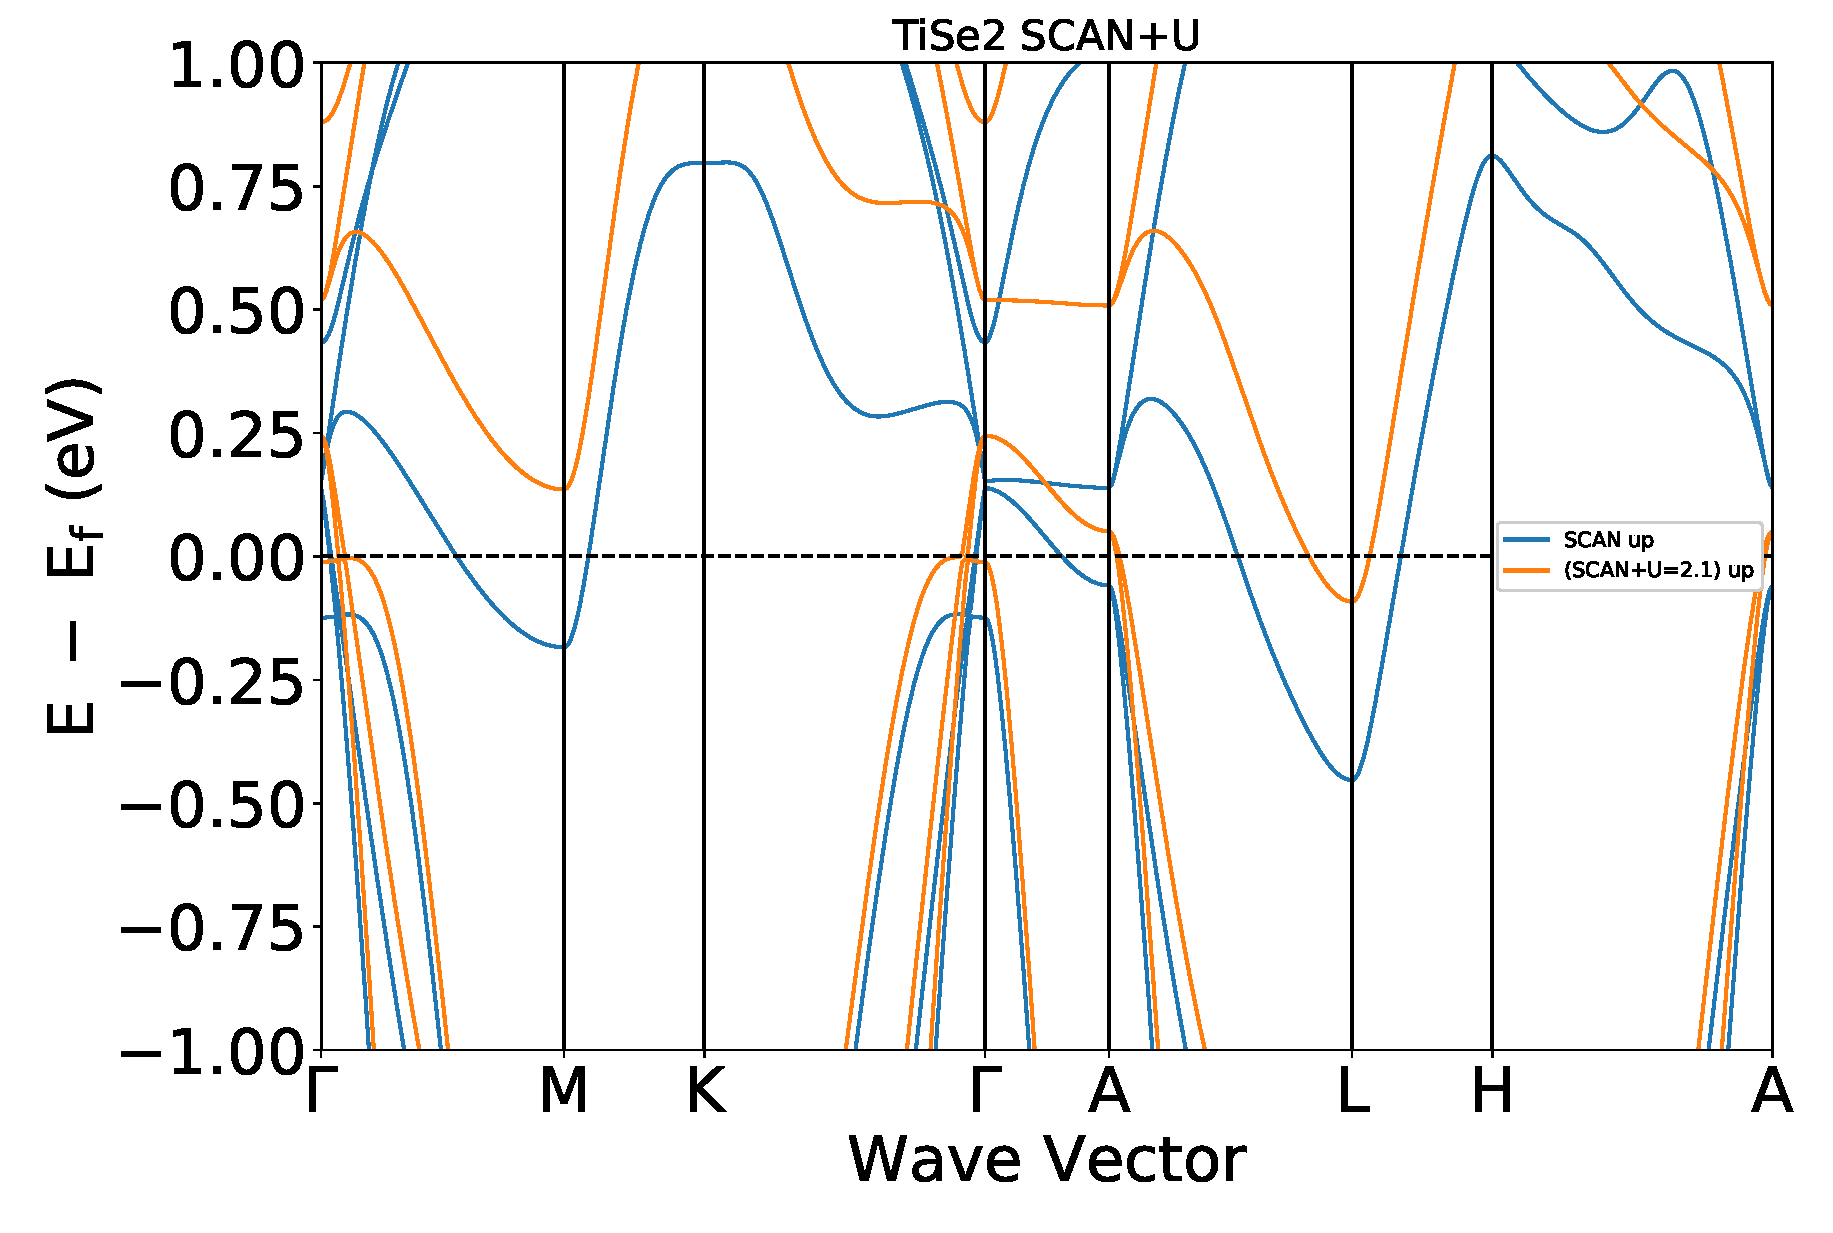
\includegraphics[scale=0.6]{results/TiSe2_SCAN_vs._SCAN+U.eps}
	\caption{Електрона будова TiSe$_2$ SCAN + U (U = 2.1).}\label{fig:SCAN+U_tise2}
\end{figure}

\begin{figure}
	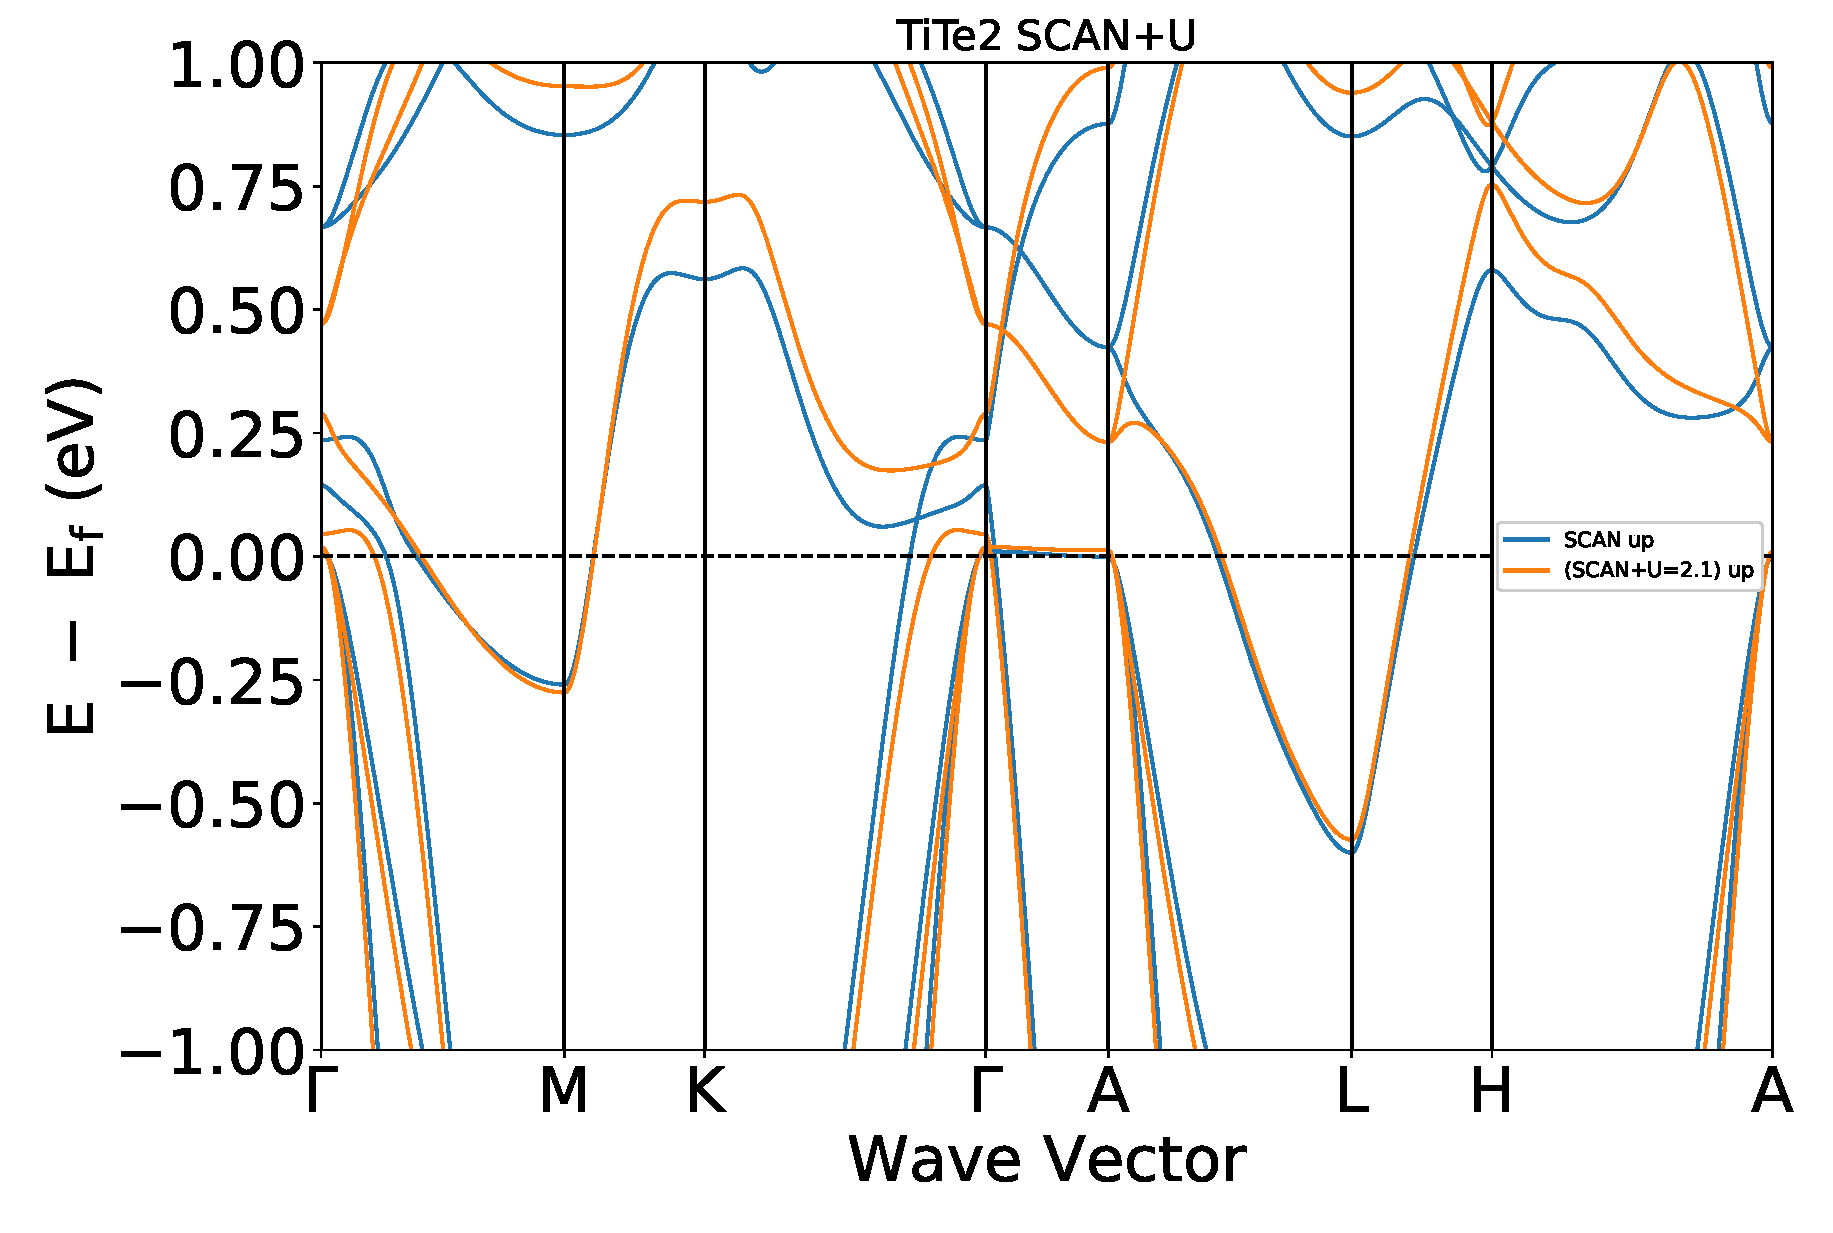
\includegraphics[scale=0.6]{results/TiTe2_SCAN_vs._SCAN+U.eps}
	\caption{Електрона будова TiTe$_2$ SCAN + U (U = 2.1).}\label{fig:SCAN+U_tite2}
\end{figure}

\section{Висновки до розділу}
У останньому розділі були представлені результати ТФГ розрахунків у SCAN наближені. Був проведений аналіз розрахунків, побудовані зони спектри та наведені таблиці постійних ґраток в порівнянні з PBE GGA функціоналом. Виявлені оптимальні значення параметра U, встановлено що U дорівнює 2.1 eV для відкриття енергетичної щілини. 
\addcontentsline{toc}{chapter}{Висновки}
\chapter*{Висновки}
Методом DFT для сполук 1T-TiX$_2$ (X = S, Se, Te) показано, що вони мають напiвметалеву природу, окрiм TiS2. Для сполук TiTe$_2$ , TiSe$_2$ встановлено перекриття мiж смугами $p$ i $d$ халькогену та титану вiдповiдно. Спостерігається збільшення піку інтенсивності DOS бiля E$_F$ при переходi вiд S до Te, Se, що обумовлено перекриттям Ti $d$ та Te, Se $p$ орбiталей у даних сполуках у значно бiльшій мірі нiж у сполуці з S.

Енергетична щiлина у сполуці TiS$_2$ задовільно описується тільки з урахуванням взаємодiї Хаббарда. Оптимальне значення U=2.1 eV вiдкриває щілину до $\approx$ 0.1 eV. Використання Ван-дер-Ваальсової поправки rVV10 наближає розрахункові результати до експериментальних значень енергетичної \\
 щілини $\approx$ 0.22 eV.
\addcontentsline{toc}{chapter}{Бібліоґрафія}
\bibliographystyle{unsrt}
\bibliography{biliog}
\end{document}
